\documentclass[11pt]{article}


%\input{meta/packages}
%
\usepackage{cite}
\usepackage[T1]{fontenc}
\usepackage{times}
\usepackage{url}
\usepackage{amsmath}
\usepackage{fancyhdr}
\usepackage{fancyvrb}
\usepackage{fancybox}
\usepackage{color}
\usepackage{colortbl}
\usepackage[table]{xcolor}
%\usepackage{tex-helpers/mathpartir}
\usepackage{amssymb}
\usepackage{xspace}
\usepackage{comment}
\usepackage{graphicx}
\graphicspath{{figures/}}
\usepackage{epsfig}
\usepackage{wrapfig}
\usepackage{multirow}
\usepackage{subfig}

% Added listing for code listings
\usepackage{listings}
\usepackage{relsize}
\usepackage{setspace}
\usepackage{sidecap}
\usepackage{algorithm}
\usepackage{algorithmic}

\textwidth=16.5cm 
\textheight=22.5cm 
\textwidth=16.5cm 
\textheight=55.5pc
\topmargin=-0.5cm 
\headsep=0cm 
\headheight=0cm 
\oddsidemargin=0cm
\evensidemargin=0cm 
\marginparwidth=0cm
\parskip=0cm
\itemsep=0.1pt
\parindent=0.5cm

%Set table separation 
\setlength{\tabcolsep}{1pt}

% Allow figures to take up the entire page
\renewcommand\floatpagefraction{.99}
\renewcommand\topfraction{.99}
\renewcommand\bottomfraction{.90}
\renewcommand\textfraction{.01}   
\setcounter{totalnumber}{50}
\setcounter{topnumber}{50}
\setcounter{bottomnumber}{50}

% formatting for grammars
%\input{tex-helpers/obey}
%\input{tex-helpers/grammar}
%\renewcommand{\nonterm}[1]{\mbox{\textit{#1}}}
\newcommand{\oneormore}[1]{#1\ensuremath{^+}}

\newcommand{\opt}[1]{\textbf{[}#1\textbf{]}}

\newcommand{\mc}[1]{\mbox{\rm \ensuremath{\text{\code{#1}}}}} 
\newcommand{\loc}{\ensuremath{\mathord{\mathit{loc}}}}
\newcommand{\ec}{\ensuremath{\mathop{\mathbb{E}}}}
\newcommand{\hole}{\ensuremath{\mathord{\mathit{-}}}}
\newcommand{\reducesto}{\hookrightarrow}

\newcommand*{\seq}[1]{\ensuremath{\left\langle {#1} \right\rangle}}
\newcommand{\config}{\seq}
\newcommand{\udot}{\mathbin{\sqcup \kern-0.53em \cdot \,}}

% Aux functions
\newcommand{\auxFunc}[1]{\ensuremath{\mathop{\mathit{#1}}}}
\newcommand{\concat}{\auxFunc{concat}}
\newcommand{\reverse}{\auxFunc{reverse}}

% Type checking macros
% change symbol type of : from mathrel 
%\DeclareMathSymbol{:}{\mathbin}{operators}{"3A} 
\newcommand{\OK}{\mbox{OK}}
\newcommand{\OKin}{\mbox{OK in }}
\newcommand{\isType}{\mbox{\textit{isType}}}
\newcommand{\isThunkType}{\mbox{\textit{isThunkType}}}
\newcommand{\isClass}{\mbox{\textit{isClass}}}
\newcommand{\Types}{\mbox{\textit{Types}}}
\newcommand{\Names}{\mbox{\textit{Names}}}
\newcommand{\TypeEnv}{\mbox{\textit{TypeEnv}}}
\newcommand{\VD}{\mbox{\textit{VD}}}
\newcommand{\TypesInOrder}{\mbox{\textit{typesInOrder}}}
\newcommand{\dom}{\mbox{\textit{dom}}}
\newcommand{\rng}{\mbox{\textit{rng}}}
\newcommand{\POWERSET}[1]{\mbox{\textit{PowerSet}}(#1)}
\newcommand{\delete}{\mbox{\textit{delete}}}
\newcommand{\mklist}{\mbox{\textit{mksupers}}}
\newcommand{\uminus}{\mbox{$\cup\!\!\!\!-$}}
\newcommand{\iminus}{\mbox{$\cap\!\!\!\!-$}}
\newcommand{\rname}[1]{$\TirName{(#1)}$} % for inline inferrule names
\newcommand{\STO}{\ensuremath{<:}}  % ``subtype of''
\newcommand{\consistent}{\ensuremath{\approx}}

% Notations 
\newcommand{\produces}{\rightsquigarrow}
\newcommand{\refinedBy}{\sqsubseteq}

% Macros for the Figure Editor Example
\newcommand{\FElement}{\mbox{\texttt{FElement}~}}
\newcommand{\ChangedFE}{\mbox{\texttt{changedFE}~}}
\newcommand{\FEChange}{\mbox{\texttt{FEChange}~}}


% Macros for defining phase transition analysis
\newcommand{\cfg}{\ensuremath{{\cal CFG}}\xspace}
\newcommand{\globTypeMap}{\ensuremath{T}\xspace}

%Redefinition of some math commands widely used outside
%mathmode
\newcommand{\memOf}{\ensuremath{\in}\xspace}

% Help LaTeX not violate the column margins
\tolerance=50000

% settings for listings
\definecolor{lightgray}{gray}{0.97}
\definecolor{darkgray}{gray}{0.5}
\definecolor{OliveGreen}{cmyk}{0.64,0,0.95,0.40}
\definecolor{DarkGreen}{cmyk}{0.58,0,0.66,0.26}
\definecolor{LightRed}{cmyk}{0,0.682,0.728,0}
\definecolor{purple}{cmyk}{0.41,0.73,0,0}

\lstset{
	language=bash, emph={},
	mathescape=false, escapechar=@,
	backgroundcolor=\color{lightgray},
	commentstyle=\color{darkgray},
	keywordstyle=\color{OliveGreen}\bfseries,
	basicstyle=\relsize{-3}\sffamily,
	numberstyle=\scriptsize\sffamily,
	emphstyle=\color{purple},
	emphstyle={[2]\color{LightRed}},
	commentstyle=\color{DarkGreen},
	stringstyle=\color{OliveGreen},
	numbers=left, stepnumber=1,
	numberblanklines=false,
	numberstyle=\tiny,
	numbersep=-3pt,
	frame=none, framexleftmargin=0pt, framexrightmargin=0pt, 
	%xleftmargin=15pt, xrightmargin=4pt,
	columns=flexible, breaklines=true,
	showspaces=false, showstringspaces=false, showtabs=false, tabsize=2,
	morekeywords={input,exists,foreach,ifall,output,of,weight,stop,visit,before,after},
	emph={int,string,bool,time,array,stack,map,visitor,%
true,false,%
top,sum,mean,maximum,minimum,set,collection,%
Project,CodeRepository,Revision,ChangedFile,ASTRoot,Namespace,Declaration,Type,Method,Variable,Statement,Expression,Modifier,%
ExpressionKind,NEW,LITERAL,EQ,NEQ,%
TypeKind,CLASS,ANONYMOUS,%
ModifierKind,OTHER,%
ChangeKind,DELETED,%
StatementKind,IF,%
RepositoryKind,SVN},
	emph={[2]isfixingrevision,getast,iskind,hasfiletype,isliteral,getsnapshot,has_modifier_public,%
format,def,len,match,lowercase,yearof,haskey,remove,strfind,push,pop},
}

% could use \relsize{-2} instead of \scriptsize below
\newcommand{\FIGCODEFONT}{\relsize{-2.5}\ttfamily}

% cross referencing
%\newcommand{\algref}[1]{Algorithm~\ref{#1}}
%\newcommand{\figref}[1]{Figure~\ref{#1}\xspace}
%\newcommand{\tabref}[1]{Table~\ref{#1}\xspace}
%\newcommand{\fignref}[1]{Figure~\ref{#1}\xspace}
%\newcommand{\secref}[1]{Section~\ref{#1}\xspace}
%\newcommand{\secnref}[1]{Section~\ref{#1}\xspace}

%\newcommand{\etal}{~\textit{et al.}\@\xspace}
\newcommand{\kind}{\textit{kind}\xspace}
\newcommand{\KIND}{\textit{KIND}\xspace}

\newcommand{\lang}{\textit{Boa}\@\xspace}

% Theorems environments...
%{theorems}
\newtheorem{theorem}{Theorem}[section]
\newtheorem{axiom}[theorem]{Axiom}
\newtheorem{corollary}[theorem]{Corollary}
\newtheorem{definition}[theorem]{Definition}
\newtheorem{example}[theorem]{Example}
\newtheorem{fact}[theorem]{Fact}
\newtheorem{lemma}[theorem]{Lemma}
\newtheorem{proposition}[theorem]{Proposition}
\newtheorem{remark}[theorem]{Remark}
\newtheorem{conjecture}[theorem]{Conjecture}
% Some helpful notation
\newcommand{\PROOF}{{\em Proof:\/}~~}
\newcommand{\PROOFSKETCH}{{\em Proof Sketch:\/}~~}
\newcommand{\QED}{\rule{0.4em}{0.65em}}

\definecolor{light-gray}{gray}{0.9}
\definecolor{very-light-gray}{gray}{0.95}

% Change section headings to look nicer
\makeatletter
\renewcommand\thesection{{\large\Alph{section}.}}
\renewcommand\section{\@startsection {section}{1}{\z@}%
                                   {-3.5ex \@plus -1ex \@minus -.2ex}%
                                   {2.3ex \@plus.2ex}%
                                   {\large\scshape\bf}}
\makeatother

\renewcommand\thesubsection{{\normalsize\Alph{section}.}{\normalsize\arabic{subsection}}}

\makeatletter
\renewcommand\subsection{\@startsection {subsection}{1}{\z@}%
                                   {-3.5ex \@plus -1ex \@minus -.2ex}%
                                   {2.3ex \@plus.2ex}%
                                   {\normalsize\scshape\bf}}
\makeatother

\renewcommand\thesubsubsection{{\normalsize\Alph{section}.}{\normalsize\arabic{subsection}.}{\normalsize\arabic{subsubsection}}}

\makeatletter
\renewcommand\subsubsection{\@startsection {subsubsection}{1}{\z@}%
                                   {-3.5ex \@plus -1ex \@minus -.2ex}%
                                   {2.3ex \@plus.2ex}%
                                   {\normalsize\scshape\bf}}
\makeatother

\newcommand\para[1]{\vspace{-1em}\paragraph{#1\ }}

% Different font in captions
\newcommand{\captionfonts}{\footnotesize}

% formatting of initial section quotations
\newcommand{\QUOTATION}[1]{\begin{flushright}\begin{footnotesize}\emph{#1}\end{footnotesize}\end{flushright}}
 
\makeatletter  % Allow the use of @ in command names
\long\def\@makecaption#1#2{%
  \vskip\abovecaptionskip
  \sbox\@tempboxa{{\captionfonts #1: #2}}%
  \ifdim \wd\@tempboxa >\hsize
    {\captionfonts #1: #2\par}
  \else
    \hbox to\hsize{\hfil\box\@tempboxa\hfil}%
  \fi
  \vskip\belowcaptionskip}
\makeatother   % Cancel the effect of \makeatletter

%\usepackage[ps2pdf,bookmarks=true]{hyperref}

\definecolor{light-gray}{gray}{0.9}
\definecolor{dark-gray}{gray}{0.7}

\newcommand\doctitle[1]{\newpage \setcounter{page}{1}\thispagestyle{fancyplain} \headheight=14pt%
                        \fancyhead[C]{\large{\bf #1}}\xspace\vspace{0.5em}}


                                                                        


\usepackage{graphicx,times}
\usepackage{wrapfig}
\usepackage{amsmath,epsfig}
\usepackage{setspace,array}
\usepackage{cite}
\usepackage{listings}
\usepackage{booktabs}
%\usepackage{bibentry}
\lstset{basicstyle=\scriptsize\sffamily,language={},frame=single,breaklines=true,columns=fullflexible,mathescape=true,escapechar=@}

\usepackage{tikz}

%\newcommand*\circled[1]{\tikz[baseline=(char.base)]{
%		\node[shape=circle,draw,inner sep=0.45pt] (char) {#1};}}


\usepackage{xspace}
\usepackage{enumitem}

\usepackage{sectsty}
\sectionfont{\large}
\subsectionfont{\normalsize}
\subsubsectionfont{\normalsize}

\usepackage[compact]{titlesec}
\usepackage[skins]{tcolorbox}

\renewcommand{\theequation}{\thesection.\arabic{equation}}
\renewcommand{\baselinestretch}{1.0}

\newcommand*\rotdia{\multicolumn{1}{R{45}{1em}}}% no optional argument here, please!
\newcommand*\rot{\rotatebox{90}}
\usepackage{multicol,multirow}

\newtheorem{Definition}{Definition}
\newtheorem{Claim}{Claim}
\newtheorem{Lemma}{Lemma}
\newtheorem{Theorem}{Theorem}
\newtheorem{Property}{Property}
\newtheorem{Problem}{Problem}


\newcommand\aName[1]{{\small\textsc{#1}}\xspace}

% cross referencing
\newcommand{\figref}[1]{Figure~\ref{#1}}
\newcommand{\secref}[1]{Section~\ref{#1}}
\newcommand{\tabref}[1]{Table~\ref{#1}}
\newcommand{\defref}[1]{Definition~\ref{#1}}

%\newcommand\aName[1]{{\small\textnormal{\textsc{#1}}}\xspace}

%\newcommand\MUBench[0]{\aName{MuBench}}
\newcommand\MUDetect[0]{\aName{MuDetect}}



\newcommand\MUBench[0]{\aName{MuBench}}
\newcommand\MUPipe[0]{\aName{MuPipe}}
\newcommand\MUC[0]{\aName{MuC}}
\newcommand\AUG[0]{\aName{AUG}}

\newcommand{\etal}{{\em et al.}}

\newcommand\GROUM[0]{\aName{GROUM}}
\newcommand\eGROUM[0]{\aName{AUG}}
\newcommand\miner[0]{\aName{AUGMiner}}

\newcommand\Colibri[0]{\aName{Colibri/ML}}
\newcommand\DroidAssist[0]{\aName{DroidAssist}}
\newcommand\GraPacc[0]{\aName{GraPacc}}
\newcommand\GROUMiner[0]{\aName{GROUMiner}}
\newcommand\Jadet[0]{\aName{Jadet}}
\newcommand\PRMiner[0]{\aName{PR-Miner}}
\newcommand\CARMiner[0]{\aName{CAR-Miner}}
\newcommand\Alattin[0]{\aName{Alattin}}
\newcommand\Tikanga[0]{\aName{Tikanga}}
\newcommand\DMMC[0]{\aName{DMMC}}
\newcommand\RGJ[0]{\aName{RGJ07}}
\newcommand\Chronicler[0]{\aName{Chronicler}}
\newcommand\Acharya[0]{\aName{AX09}}

\newcommand{\checkNum}[1]{#1}

\newcommand{\revise} {\bf}

\newcommand{\code}[1]{{\scriptsize\texttt{#1}}}
\newcommand{\op}{\tau}
\newcommand{\refac}{\rho}
\newcommand{\edit}{\sigma}
\newcommand{\T}{\theta}
\newcommand{\comp}{;}
\newcommand{\pre}{\prec_P}
\newcommand{\meth}{KSISA}

\newcommand{\MyParagraph}[1]{\textbf{#1}{ }}
\newcommand{\fixme} [1] {\textcolor{red}{{\it FIXME}: #1}}

\usepackage{vmargin}
\setpapersize{USletter}
\setmarginsrb{1.0in}{1in}{1.0in}{1in}%
           {0pt}{0mm}{0pt}{10mm}
\newcommand{\remove}[1]{}



\usepackage{tweaklist}
\renewcommand{\enumhook}{\setlength{\topsep}{0pt}%
  \setlength{\itemsep}{0pt}}
\renewcommand{\itemhook}{\setlength{\topsep}{0pt}%
  \setlength{\itemsep}{0pt}}
\renewcommand{\descripthook}{\setlength{\topsep}{0pt}%
  \setlength{\itemsep}{0pt}}


\usepackage{tikz}
\usetikzlibrary{patterns}
\newcommand*\circled[1]{\tikz[baseline=(char.base)]{
            \node[shape=circle,draw,inner sep=1.5pt] (char) {#1};}}
%\newcommand{\david}[1]{\textcolor{red}{{#1}}}

\usepackage{fdsymbol}
\usepackage{tikz}
\usepackage{pgfplots}
\usetikzlibrary{
        shapes,
    }
\pgfplotsset{compat=1.9}
\usepackage{listings} %For code in appendix
\lstset
{ %Formatting for code in appendix
    language=Matlab,
    basicstyle=\footnotesize,
    numbers=left,
    stepnumber=1,
    showstringspaces=false,
    tabsize=1,
    breaklines=true,
    breakatwhitespace=false,
}
% We will externalize the figures
%\usepgfplotslibrary{external}
\usepgfplotslibrary{groupplots}
%\tikzexternalize

\definecolor{dkgreen}{rgb}{0,0.6,0}
\definecolor{meatbrown}{rgb}{0.9, 0.72, 0.23}
\definecolor{lightgray}{rgb}{211, 211, 211}

%\newcommand\Tone{Thrust 1 (T1). Ongoing Evaluation of Existing Code Representation Learning in Bug Detect-Fix Processes}
\newcommand\Tone{Thrust 1 (T1). Design Framework and Environment for Code Representation Learning (CRL): Representations, Models, and Methodologies}

\newcommand\Ttwo{Thrust 2 (T2). Quality Evaluation Framework for Code Representation Learning}

\newcommand\Tthree{Thrust 3 (T3). Applications of CRL Framework in Bug Detection, Testing, Fault Localization, and Auto Program Repair}

%Enhancing Techniques in the Bug Fixing Process with Deep Learning}

% all tool names used in this proposal

%\newcommand\tool{NeuralPPA}

\newcommand{\tool}{\textsc{FuzzWise}\xspace}

\newcommand{\deeppda}{\textsc{DeepPDA}\xspace}

\newcommand\deepbugs{\textbf{DeepBugs}~\cite{Pradel-2018}}
\newcommand\bugram{\textbf{Bugram}~\cite{Wang-2016}}
\newcommand\narminer{\textbf{NAR-miner}~\cite{Bian-2018}}
\newcommand\findbugs{\textbf{FindBugs}~\cite{ayewah-2007}}
\newcommand\deepsim{\textbf{DeepSim}\cite{Zhao-2018}}
\newcommand\codetovec{\textbf{code2vec}\cite{Alon-2018}}
\newcommand\codevectors{\textbf{CodeVectors}\cite{Henkel-2018}}
\newcommand\dlsim{\textbf{DL-Sim}~\cite{Tufano-2018}}
\newcommand\treelstm{\textbf{Tree~LSTM}~\cite{Tai-2015}}

\newcommand\cnn{CNN~\cite{kim2014convolutional}}



% auto-fix
\newcommand\CODIT{\textbf{CODIT}~\cite{chakrabortycodit}}
\newcommand\Ratchet{\textbf{Ratchet}~\cite{hata2018learning}}
\newcommand\Tufano{\textbf{Tufano}~\cite{tufano2019learning}}
\newcommand\CoCo{\textbf{CoCoNut}~\cite{lutellier2020coconut}}

% FL
\newcommand\MLP{\textbf{MLP}~\cite{bourlard1988auto}}

\pagestyle{empty}

\begin{document}

\begin{center}
%{\large \bf Collaborative Research: SHF: Small: Innovations in Deep Learning to Enhance Program Analysis and Representations to Improve Bug Fixing Process}

%{\large \bf Collaborative Research: SHF: Small: Connecting Deep Learning and Program Analysis to Improve Bug Detecting and Fixing Processes through Code Representation Learning}

{\large \bf SHF: Small: Predictive, Coverage-Guided, Intelligent Fuzzing Approach}
\end{center}
\vspace{-.1in}
\hrule

%\section{Introduction}



%%\subsection{Problem Description}


Developers often use online question and answering (Q\&A) forums,
e.g., StackOverflow (S/O), to learn how to use software libraries and
frameworks. Sometimes, the answer to a question comes as a
fragment/chunk of code, which later makes it to the production
applications, stemming from the copy-and-paste software reuse
practice. Unfortunately, if the copied code fragments are vulnerable,
i.e., possess defects that can potentially be exploited, it will lead
to the applications being prone to attacks. Verdi {\em et
  al.}~\cite{verdi-tse22} reviewed more than 72K C++ code snippets
that migrated from 1,325 S/O answers. Of these, they reported a total
of 99 vulnerable code snippets of 31 different types that made their
way to 2,589 GitHub repositories. Thus, it is crucial to detect early
the vulnerabilities in the code snippets from online forums.
%Running a vulnerability detection tool on the source code after the
%integration of a S/O code snippet into the current codebase would
%waste developers' effort for such integration.

Security researchers have proposed several automated approaches for
vulnerability detection (VD) using program
analysis~\cite{FlawFinder,RATS,viega2000its4,Checkmarx,HPFortify,Coverity,BufferOverFlow,SQLInj,Cross-siteScripting,AuthBypassSpoofing},
as well as machine learning (ML) including deep learning
(DL)~\cite{fse21,chakraborty2020deep,zhou2019devign,li2018sysevr,li2018vuldeepecker}
techniques. However, these approaches warrant the code to exist as
complete program units, often making use of program representations
such~as abstract syntax tree (AST), Program Dependence Graph
(PDG)~\cite{fse21,li2018vuldeepecker}, Control Flow Graph
(CFG)~\cite{zhou2019devign}, Data Flow Graph
(DFG)~\cite{zhou2019devign}, Code Property Graph
(CPG)~\cite{chakraborty2020deep}, etc. At a minimum, they operate at
the method-level granularity, making it impossible to utilize them for
directly detecting vulnerabilities in code snippets. A possible
alternative would be to plug the code snippet into the method, resolve
any ambiguities, and test it with a VD tool. However, such a strategy
is limited. First, if found vulnerable, the efforts of integrating the
code snippet into the existing method would be lost. Second, due to
the black-box
%(inexplicable?)
nature of DL models, we would not know the origin of the
vulnerability, i.e., whether it arises due to the flawed code snippet
or the existing part of the code.

%other statements in the method.

%Besides, even a commit-level VD model requires the code before/after changes to be syntactically valid to extract those features.

Importantly, analyzing code snippets is not straightforward as they
are often incomplete, un-parseable, contain declaration/reference
ambiguity, and are interspersed between user comments. Currently,
there exist tools such as PPA~\cite{ppa08},~which parse an incomplete
code fragment to build the AST and~ex\-tract data types in a
best-effort manner, while StaType \cite{icse18} resolves the libraries
and recovers only the fully-qualified names for references. However,
the basic infrastructure for partial program analysis on incomplete
code snippets is not yet possible. The infrastructure includes the
fundamental supports/services such as lexical, syntactic, and semantic
analysis so that the static and dynamic analysis techniques could be
built upon. Let us call such an infrastructure, {\em partial program
analysis infrastructure}.

In addition to vulnerability detection, such partial program analysis
infrastructure is also beneficial to the other software engineering
(SE) tasks that can tolerate a low level of errors and imprecision in
building the program representations. For example, consider code
completion~\cite{codefill-icse22,facebook-icse21}, in which a model
provides suggestions to complete partial code. Existing ML/DL-based
code completion models are just based on the code sequences or utilize
the syntactic structure in ASTs, but none leverage the program
dependencies due to the nature of partial code. Next, consider the
task of analyzing the code fragments in a bug report to connect it to
the relevant source files for bug localization
purposes~\cite{euler-fse19,icpc17}. Here too, a need for partial
program analysis, especially for partial program dependence analysis,
can be observed.









%\section{Introduction}
Integrating the utilization of program analysis (PA) tools early in the development process of modern, large-scale software systems is crucial in determining the weaknesses/vulnerabilities in the code. Consider, for instance, a scenario in which a developer wants to use an online question and answering (Q\&A) forum, e.g., StackOverflow (S/O), to learn how to use software libraries or frameworks. Typically, the answer to a posed question comes as a fragment/chunk of code, which later makes it to the production application, stemming from the copy-and-paste software reuse practice. Unfortunately, if the copied code fragment is vulnerable, i.e., possesses defects that one can potentially exploit, it will result in the application being prone to attacks. Verdi {\em et al.}~\cite{verdi-tse22} reviewed more than 72K C++ code snippets that migrated from 1,325 S/O answers, reporting a total of 99 vulnerable code snippets of 31 different types that made their way to 2,589 GitHub repositories.

Security researchers have proposed several automated approaches for vulnerability detection (VD) in software systems using program analysis (PA)~\cite{FlawFinder,RATS,viega2000its4,Checkmarx,HPFortify,Coverity}, as well as machine and deep learning (ML \& DL) \cite{fse21,chakraborty2020deep,zhou2019devign,li2018sysevr,li2018vuldeepecker} techniques. These approaches typically leverage program representations such as abstract syntax tree (AST), program dependence graph (PDG)~\cite{fse21,li2018vuldeepecker}, control-flow graph (CFG)~\cite{zhou2019devign}, data-flow graph (DFG)~\cite{zhou2019devign}, code property graph (CPG)~\cite{chakraborty2020deep}, etc., to model the vulnerable features. 
%However, extending such analyses to code snippets is not straightforward as they are often incomplete, unparseable, contain declaration/reference ambiguity, and may be interspersed between user comments. Currently, there exist tools such as PPA~\cite{ppa08}, which parse an incomplete code fragment to build the AST and extract data types in a best-effort manner, while StaType \cite{icse18} resolves the libraries and recovers only the fully-qualified names for references. However, the basic infrastructure for partial program analysis, i.e., for analyzing incomplete code is not yet available. 
%Such an infrastructure must include fundamental supports/services at the structural, semantic, and execution levels, thus enabling the static and dynamic analysis techniques to be built upon. 
%Let us refer to this as \textit{partial program analysis infrastructure}.
However, the PA tools employed to derive these program representations warrant the code to exist as complete program units, at the very least, at the method-level granularity. As a result, it is impossible to utilize such VD tools to find vulnerabilities in code snippets. A possible alternative would be to plug the code snippet into the method, resolve any ambiguities, and test it with a VD tool. However, such a strategy is limited. First, if a vulnerability is found, the efforts of integrating the code snippet into the existing method would be lost. Second, due to the black-box nature of DL models, we would not know the origin of the vulnerability, i.e., whether it arises due to the flawed code snippet or the existing part of the code.

Besides, analyzing code snippets is not straightforward as they are often incomplete, un-parseable, contain declaration/reference ambiguity, and may be interspersed between user comments. Currently, there exist tools such as PPA~\cite{ppa08},~which parse an incomplete code fragment to build the AST and extract data types in a best-effort manner, while StatType \cite{icse18} resolves the libraries and recovers only the fully-qualified names for references. However, the basic infrastructure for partial program analysis, i.e., for analyzing incomplete code is not yet available. Such an infrastructure must include fundamental supports/services at the structural and semantic levels, thus enabling the program analysis techniques to be built upon. Let us refer to this as \textit{partial program analysis infrastructure}.


In addition to vulnerability detection, such an 
%partial program analysis infrastructure 
infrastructure
is also beneficial to other software engineering (SE) tasks that can tolerate a low level of errors and imprecision in building program representations. For example, consider code completion~\cite{codefill-icse22,facebook-icse21}, in which a model provides suggestions to complete partial code. Existing state-of-the-art ML/DL-based code completion models are just based on the code sequences or utilize the syntactic structure in ASTs, but none leverage the program dependencies due to the nature of partial code. Next, consider the task of analyzing the code fragments in a bug report to connect it to the relevant source files for bug localization purposes~\cite{euler-fse19,icpc17}. Here too, a need for partial program analysis, specifically partial program dependence analysis, can be observed.

The other facets of program analysis tools that need to be considered are their soundness and completeness. For example, static analysis tools are designed to detect errors that are valid for all possible executions, which often come at the cost of multiple approximations. As a result, such tools tend to overestimate, resulting in false positives. Next, consider the task of symbolic execution, which is limited by the path explosion problem that hinders its applicability to large-scale software systems. The effectiveness of such a symbolic execution engine can be improved by enhancing the symbolic constraints of the variables, and by guiding it to explore the right subset of symbolic states. 

%While the state-of-the-art research and practice has been well-established for the analysis of the entire programs, very little research and knowledge has been achieved for partial program analysis.

To this effect, we set out to investigate {\tool}, a {\em \underline{Neural} Network-Based \underline{P}rogram \underline{A}nalysis} infrastructure. We aim to establish {\em a scientific foundation, novel methodologies, frameworks, models, and algorithmic solutions for neural program analysis}. We address two major issues in Program Analysis:

(1) {\bf Enabling analysis of incomplete code fragments}, i.e.,
partial program analysis;

(2) {\bf Empowering existing PA tools by making them more sound and
  complete} (Figure~\ref{fig:arch}). {\tool} will allow the
construction of efficient program analysis techniques for (partial)
code on which downstream software engineering applications can be
built.


\subsection{Research Objectives and Anticipated Results}

\begin{figure}[t]
    \centering
    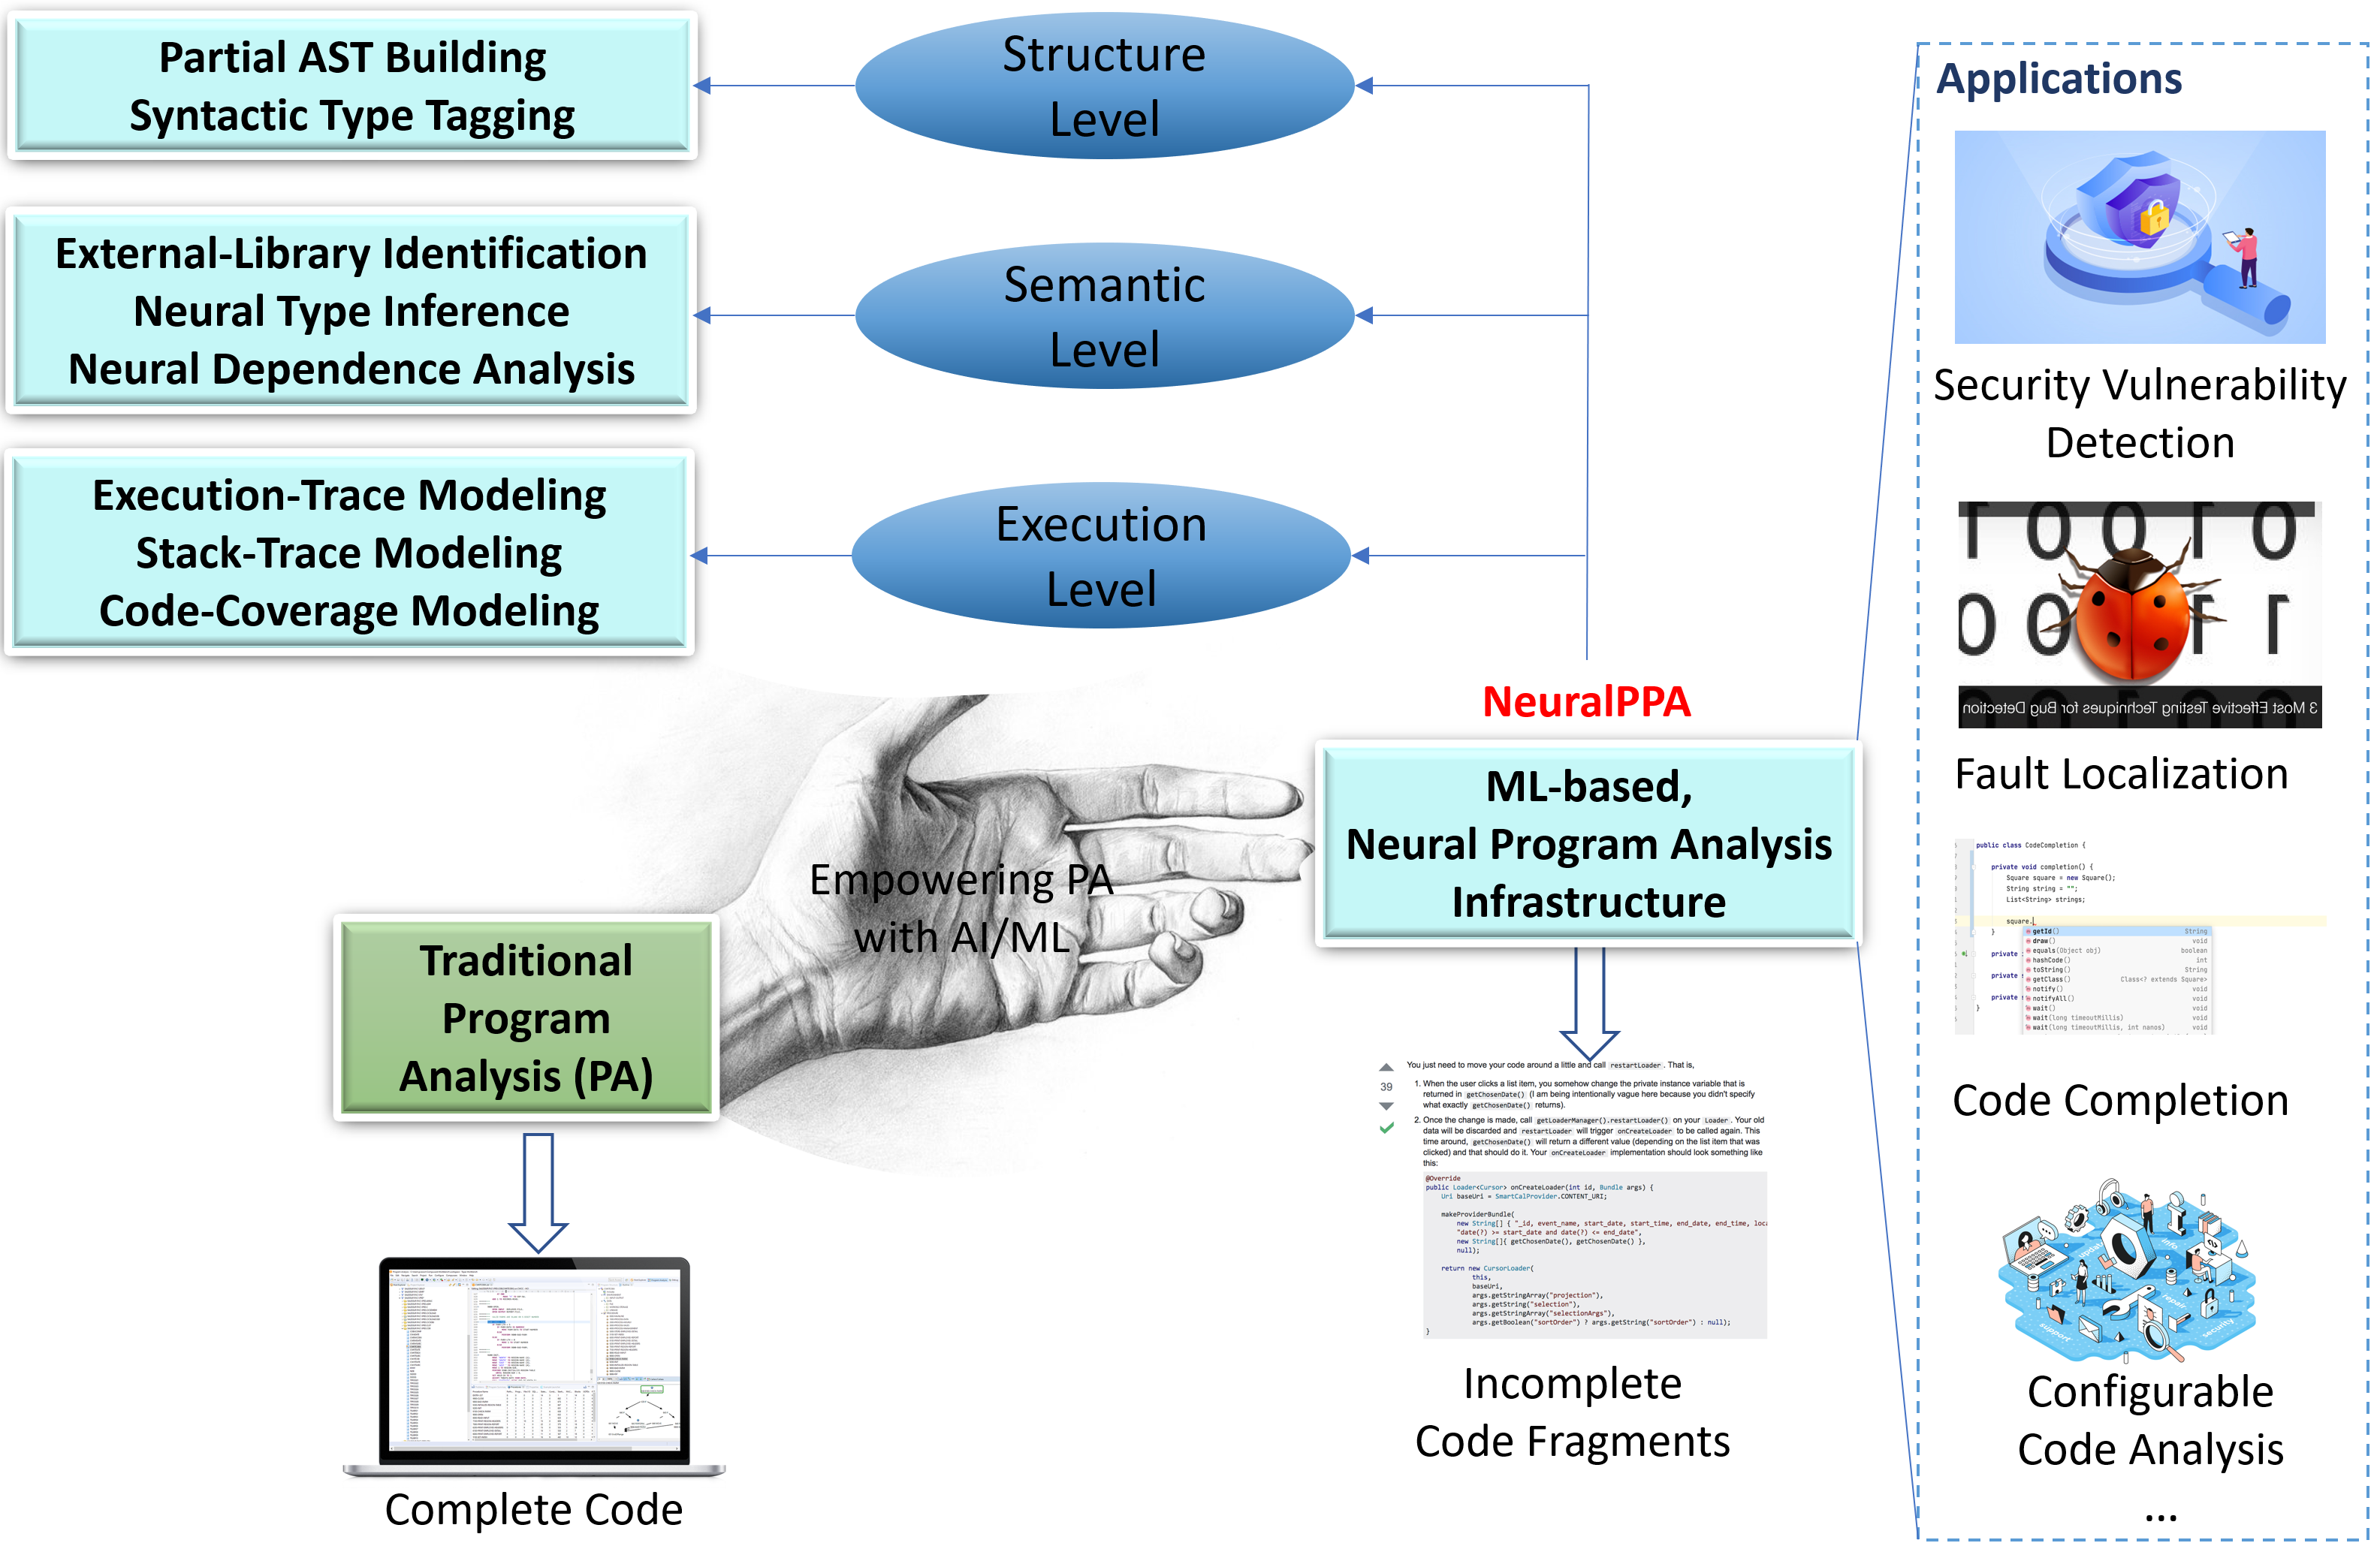
\includegraphics[width=0.9\textwidth]{graphs/neuralppa}
    \vspace{-12pt}
    \caption{{\tool}: Machine Learning-based Program Analysis Infrastructure}
    \label{fig:arch}
\end{figure}


While the state-of-the-art research and practice has been
well-established for the analysis of the entire programs, very little
research and knowledge has been achieved for partial program
analysis.
%
In this proposal, we set out to investigate and develop {\tool}, a
{\em \underline{Neural}-network-based \underline{P}artial
  \underline{P}rogram \underline{A}nalysis infrastructure}. We aim to
develop {\bf a scientific foundation, novel methodologies, frameworks,
  models, and algorithmic solutions for neural partial program
  analysis}. {\tool} {\bf enpowers program analysis (PA) with advanced
machine learning (ML) and artificial intelligence (AI) to enable the
program analysis on incomplete code fragments} (Figure~\ref{fig:arch}).
{\tool} will allow the constructions of the program analysis
techniques for partial code on which downstream software
engineering applications can be built.


In this work, our key philosophy is that {\em the analysis of
  partial code can be learned from the analysis of entire programs in
  the wealth of information from ultra-large-scale, open-source
  software repositories}.



Specifically, we draw our motivation for such a data-driven,
learning-based approach from the following. First, ultra-large-scale
software repositories, e.g. GitHub (7M+ projects) and SourceForge
(700k+ projects) contain an enormous collection of programs. These
repositories amount to 1,000,000,000+ lines of code, 10,000,000+
revision logs, and 3,000,000+ issue reports. This wealth of knowledge
is an excellent source for {\tool}. Hindle {\em et
  al.}~\cite{naturalness-icse12} have shown that code has high
repetitiveness and predictability, and can be captured well by
statistical models. Thus, we expect to build ML models to learn from
those repositories. Second, in an empirical study on the
repetitiveness, containment, and composability of PDGs in open-source
projects, the PI group~\cite{msr16} reported that among
17.5M PDGs with 1.6B PDG subgraphs, 14.3\% of the PDGs have all of
their subgraphs repeated across different projects. Furthermore, in
15.6\% of the PDGs, at least 90\% of their subgraphs are likely to
have appeared before in other projects. Thus, {\tool} could learn from
PDGs with complete program dependencies retrieved from existing code
repositories and derive the dependencies for the (partial) code
fragment under study. The PI group also reported a high repetitiveness
level for AST code structure in open-source
projects~\cite{icse15}. Finally, such a program analysis
infrastructure like {\tool} can be drawn from the spirit and successes
of the approaches in natural language processing (NLP). For example,
at the lexical level, the task of deriving the token types for source
code tokens could be analogous to the part-of-speech (PoS) tagging in
NLP. At the syntax level, the task of learning the syntactic structure
in AST of the partial code can be inspired by the approaches to build
parse trees for natural-language texts. At the semantic level, the
partial program dependence analysis infrastructure is similar in
spirit to the the neural network-based dependency parsing in NLP,
which learns the dependencies signifying the semantic relationships
between words in a sentence from text corpora.

Toward this theme, in our preliminary work, we developed DeepPDA, a neural
network-based partial program dependence analysis approach that learns
to derive the program dependencies for any code fragments (i.e., both
complete and incomplete). In our preliminary empirical evaluation, we
intrinsically evaluated it on Java and C/C++ programs. First, we
trained {\tool} on complete code. For testing, we treated each method
individually and chose a consecutive portion within the method to
predict the program dependencies, and compared them against the actual
dependencies. Overall, DeepPDA predicts CFG and PDG edges in Java
with an F-score of 94.29\%, and in C++ with an F-score of
92.46\%.
%
We also developed as an approach to derive the data
types of the variables in the code snippets. We treat the problem as
statistical machine translation from source code with partially
qualified names to source code with FQNs of the APIs. Our empirical
evaluation on real-world code and StackOverflow posts shows that our
technique achieves high accuracy with 97.6\% precision and 96.7\%
recall in deriving data types in code snippets.


In {\tool}, we propose the following thrusts of research
(Table~\ref{tab:milestones}):

\vspace{3pt}
\noindent \textbf{Thurst 1. Neural Structural Analysis Infrastructure
  \code{NeuralStruct}.} ({\em Section~\ref{}}) Source code has
well-defined structures and semantics. Thus, the basic infrastructure
in {\tool} is the neural structural analysis (\code{NeuralStruct})
component.  This component has two main tasks. First, it learns from
the syntactic structures of the complete code in the training dataset
collected from large-scale code repositories, to derive the abstract
syntax tree (AST) that best represents the syntactic structure of the
given partial code, i.e., with the highest likelihood/probability.
The traditional lexical analyzer still works for partial code due to
the independence nature of lexical tokens. The second task of this
component is to tag the code tokens with the types of the syntactic
units including the statement types (\code{if}, \code{for}, etc.),
variables, fields, methods, classes, etc. Both of the tasks can be
performed with our learning-based approaches in a dual-learning
manner.
  
\vspace{3pt}
\noindent \textbf{Thurst 2. Neural Semantic Analysis Infrastructure.}
({\em Section~\ref{}}) The basis components for several program
analysis techniques include the following:

1) the identification of the APIs of the external libraries in the
external references in the partial code: this is needed because the
partial code contains the undeclared reference and/or
declaration/reference ambiguity without explicit declaration of the
APIs in the external libraries.

2) the inference of the type information for the entities in the
partial code: due to the ambiguity in the declaration, the types of
the variables and statements are not always obviously defined. Thus,
the type inference is a basic service within {\tool}.

3) the inference of the program dependencies among the statements in
the partial code: several program analysis techniques are based on the
program dependencies, which are not always obtainable due to the
incompleteness of the given code fragment.

\vspace{3pt}
\noindent \textbf{Thurst 3. Neural Symbolic Execution Infrastructure.}
...

\vspace{3pt}
\noindent \textbf{Thurst 4. Neural Partial Program Analysis
  Applications.}  ({\em Section~\ref{}}) Our last thrust of research
is aimed to evaluate our basic partial program analysis infrastructure
in a few applications. We choose the following software engineering
applications: 1) software vulnerability detection for code snippets,
2) fault localization, and 3) code completion.

\vspace{3pt}
\noindent \textbf{Thurst ???. Neural Execution Analysis Infrastructure.}
({\em Section~\ref{}}) All the dynamic analysis techniques require the
analysis and understanding of the execution. However, for an
incomplete code, we first need to design a component that can wrap
around the given code fragment with the minimum code so that the code
fragment can be executed. When the code is executed, we also need the
approaches that represent the executed statements and their relations,
model the execution and stack traces, and model the code coverages
for an execution.


\begin{table*}[t]
	\vspace{-15pt}
\begin{center}
{\footnotesize{
\begin{tabular}{cc}
\begin{tabular}[t]{|p{0.2in}|p{2.95in}|} 
\hline
\multicolumn{2}{|>{\columncolor[gray]{0}}c|}{\textcolor{white}
{\bf Year 1 Project Milestones \& Deliverables}}\\
\hline 
\hline
\multicolumn{2}{|c|}{\bf T1. Neural Structure Analysis Infrastructure}\\
\hline
{\bf 1.1} & Neural Syntactic Type Tagging\\
{\bf 1.2} & Neural Partial AST Building\\
{\bf 1.3} & Evaluation of the components\\
\hline
\hline
\multicolumn{2}{|c|}{\bf T2. Neural Semantic Analysis Infrastructure}\\ 
\hline
{\bf 2.1} & External-Library Identification\\
\hline
%\hline
%\multicolumn{2}{|c|}{\bf Integrate Code Synthesis into Tools}\\
%\hline
%{\bf 1.5} & \goalOneFour.\\
%\hline
\multicolumn{2}{c}{}
\end{tabular}
&
\begin{tabular}[t]{|p{0.2in}|p{2.95in}|} \hline
\multicolumn{2}{|>{\columncolor[gray]{0}}c|}{\textcolor{white}
{\bf Year 2 Project Milestones \& Deliverables}}\\
\hline 
\hline
\multicolumn{2}{|c|}{\bf T2. Neural Semantic Analysis Infrastructure}\\
\hline
{\bf 2.2} & Neural Type Inference\\
{\bf 2.3} & Neural Dependence Analysis\\
%{\bf 2.3} & Integrate Evaluation Framework into Design Environment\\
%{\bf 2.4} & Evaluate CRL Framework with Existing Models\\
%{\bf 2.3} & \goalTwoThree.\\

\hline
\hline
\multicolumn{2}{|c|}{\bf T3. Neural Execution Analysis}\\ 
\hline
%{\bf 3.1} & Design New Code Representations and Learning Models.\\
{\bf 3.1} & Neural Execution-Trace Modeling\\
%{\bf 2.4} & Advance FL and RT-CI Approaches.\\
%{\bf 2.5} & Advance Regression Testing in CI Approaches.\\
%{\bf 2.5} & Advance APR Approaches with Framework.\\
\hline
%\hline
%\multicolumn{2}{|c|}{\bf Community Involvement: Capacity Building}\\
%\hline
%{\bf 2.4} & \goalTwoFour.\\
%{\bf 2.5} & \goalTwoFive.\\
%{\bf 2.6} & \goalTwoSix.\\
%\hline
\multicolumn{2}{c}{}
\end{tabular}
\end{tabular}\\
\vspace*{-.3cm}
\begin{tabular}{c}\hline
\multicolumn{1}{|>{\centering\columncolor[gray]{0}}p{6.44in}|}{\textcolor{white}
{\bf Year 3 Project Milestones \& Deliverables}}\\
\hline
\end{tabular}\\
\vspace*{-.2cm}
\begin{tabular}{cc}
\begin{tabular}[t]{|p{0.2in}|p{2.95in}|}
\hline
\multicolumn{2}{|c|}{\bf T3. Neural Execution Analysis}\\
\hline
{\bf 3.2} & Neural Stack Trace Modeling\\
{\bf 3.3} & Neural Code Coverage Modeling\\

%{\bf 3.3} & Testing on Models in IDE tools.\\
\hline
%\hline
%\multicolumn{2}{|c|}{\bf \goalTwo}\\ 
%\hline
%{\bf 3.3} & \goalThreeThree.\\
%\hline
\multicolumn{2}{c}{}
\end{tabular}
&
\begin{tabular}[t]{|p{0.2in}|p{2.95in}|}
\hline
\multicolumn{2}{|c|}{\bf T4. Neural Partial Program Analysis Applications}\\
\hline
%{\bf 3.1} & Design New Code Representations\\

{\bf 4.1} & Security Vulnerablity Detection with {\tool}\\
{\bf 4.2} & Fault Localization and Completion with {\tool}\\

\hline
\multicolumn{2}{c}{}
\end{tabular}
\end{tabular}
\vspace{-15pt}
}}
\end{center}
\vspace*{-.3in}
%\caption{Tasks and Milestones. (Rep. = Representation)}
\caption{The 3-year schedule of Thrusts, Tasks, and Milestones of this proposal.}
%the schedule of Thrusts, Tasks, and Milestones of this proposal.
%\vspace{-10pt}
\label{tab:milestones}
\vspace{-10pt}
\end{table*}
%






%\subsection{Significance of This Proposed Project: NSF Merit Criteria}

\section{Intellectual Merits}

The results of this project will advance the state-of-the-art
knowledge and scientific foundations in both program analysis and
machine learning. They are transformative and directly help improve
software quality with novel program analysis and vulnerability
detection tools.

\noindent \underline{{\bf Advance the state-of-the-art knowledge and
    understanding}}. Neural program analysis infrastructure in Thrusts
1--3 will advance the body of knowledge and theoretical foundations
for machine learning and AI for code. Thrust 4 will help advance the
practical tools for software security and engineering.

\noindent \underline{{\bf Scientific foundation, creative/original
    research}}. This project will provide a scientific
foundation (novel concepts, representations, algorithms, models,
and tools) (1) to enable the analysis on partial code, (2) to empower
the program analysis techniques on both (in)complete code,
and (3) to enable the applications of program analysis on incomplete
code such as vulnerability detection on code snippets, code
completion, etc.

\section{Broader Impacts}

\underline{{\bf (1) Transformative and benefits to society}}. Our
results will be transformative and directly benefit to our society.
They will lead to increasing developers' productivity, software
quality \& reliability.  Our validation involves students and
professionals, promoting teaching, training, and learning of both {\bf
  program analysis} and {\bf machine learning} techniques that
have wide impacts in industry and academic communities.

\noindent\underline{{\bf (2) Foster other related research
    activities}}. Our results will foster {\em research activities in
  related fields of {\bf deep learning} and {\bf software
    security}}. This project will produce theoretical concepts and
techniques that are novel even in deep learning, e.g., novel neural
networks to model and learn for code. The applications of our neural
program analysis in software engineering applications will advance
software security and reliability.

%The collected {\bf large scale bug\&fix corpus} will be useful for
%software quality and reliability research.
%Innovations in CRL could be used to {\bf advance other SE tasks}. We
%will also develop {\bf novel DL-based bug detect-fix} approaches.


\noindent\underline{{\bf (3) Education, dissemination, and broader participation}} (Section~\ref{edu}). The
research will enhance the infrastructure for teaching/research via
tools and data sets for use by students and practitioners, and for
enhancement by researchers. We will provide related learning
modules for educators as well. It will include outreach activities for
undergraduate students, underrepresented groups, minorities, and women
in science.
%contribute novel
%teaching modules to our curriculum.
%Details will be presented in Section~\ref{edu}


\iffalse
\begin{itemize}
	\vspace{-5pt}
\itemsep-0.2em 
  \item {\bf Transformative and benefits to society}. Our 
    results will be transformative and directly benefit to our
    society. 
    They will lead to increasing developers' productivity
    and software quality \& reliability. 
    Our validation involves students and
    professionals, promoting teaching, training, and learning of bug detecting and fixing techniques that have wide impacts 
    in industry and academic communities.

%report

  \item {\bf Foster other research activities}. Our results will
    foster research activities in related fields of deep learning and
    software quality. 
    This project will produce theoretical
    concepts and techniques that are novel even in deep learning, e.g.,
    novel neural networks for modeling and learning code. 
    The collected large scale bug fixing corpus will be useful for software quality and reliability research in general.
    %e.g.,   code transformation. 
%    This project will also advance
%    the state-of-the-art research in large-scale program analysis with
%    deep neural network models.

%The representation for software security vulnerabili will be useful in
%research on software security, malware detection, vulnerability
%reports, and automatic security patching.


  \item {\bf Education, dissemination, and broader participation}.
  The research will enhance the infrastructure for teaching and
  research by providing tools and data sets for use by students and
  practitioners, and for enhancement by other researchers. We will
  provide related learning modules for educators as well. It will
  contribute novel teaching modules to our curriculum. Details will be
  presented in Section~\ref{edu}

%Details are in Section 4.

\end{itemize}
\fi


\section{Introduction}
\label{sec:intro}

Software testing is a crucial aspect in software development, ensuring
that applications function correctly, meet requirements, and provide a
reliable and secure user experience. Among various testing methods,
{\bf fuzz testing} (or {\bf fuzzing}) involves providing random or
semi-random data inputs to a program in an attempt to trigger
unforeseen behaviors, crashes, or security flaws. Unlike traditional
testing methods that rely on predefined inputs, fuzz testing involves
automatically generating a wide range of random, unexpected, or
malformed inputs to the system under test. This approach is invaluable
for uncovering obscure bugs and security flaws that might be missed by
other testing strategies. By exposing software to a diverse set of
inputs, fuzz testing can reveal how the application handles unexpected
conditions, thus identifying potential points of failure or security
vulnerabilities. This is particularly important for security-sensitive
applications where robustness against unusual or malicious inputs is
essential.

%Overall, fuzz testing enhances the reliability and security of software by proactively identifying and addressing issues that could lead to crashes, data corruption, or breaches.

Among fuzzing methods, a {\em coverage-guided fuzz testing framework}
is a systematic approach to identifying software defects or
vulnerabilities through automated
testing. Figure~\ref{fig:coverage-fuzz} illustrates its process. The
first stage, which is the {\em seed corpus generation}, starts with
creating an initial set of test cases, known as the seed~corpus. These
test cases are typically generated manually or extracted from existing
test suites, real-world inputs, or example code snippets. Through a
selection, each test case in the seed corpus is chosen for the second
stage: {\em fuzzing input generation}. In this stage, the fuzzing
engine generates a large number of mutated or random inputs based on
the seed corpus. These inputs are designed to explore various paths
and edge cases within the target program under test. In the third
stage, {\em target program execution}, the generated inputs are fed
into the target program. It executes the inputs and processes them
according to its normal operation. During this stage, the framework
{\em monitors code coverage}, tracking which parts of the target
source code are exercised by the inputs. This is typically done using
instrumentation techniques or by analyzing execution traces. During
execution, if the execution of an input triggers an unexpected
behavior, e.g., a crash, assertion failure, or memory corruption, the
framework identifies it as a potential defect. The detected faults are
logged and reported to developers for further investigation
and~resolution.

In the next stage ({\em feedback loop}), the framework selects the
best test cases with highest code coverages and adds them back to the
seed corpus/pool. The framework continuously mutates and generates new
inputs based on the coverage feedback and best test cases received
for the target program. The inputs that explore previously untested
paths or trigger new code coverage are prioritized for further
mutation and testing. The fuzzing process iterates continuously,
generating new inputs, executing them against the target program, and
refining the test cases based on the coverage feedback. As the process
progresses, the framework may analyze and prioritize inputs based on
factors such as code coverage, execution time, and the severity of
detected faults. This helps focus testing efforts on the most
promising areas of the codebase.

Despite its popularity and successes, the coverage-guided fuzzing
framework still has the following key shortcomings. First, the
framework might suffer the issue of inefficiency and high resource
consumption: it generates a large number of test cases without prior
knowledge of their code coverage quality. This can lead to inefficient
resource and time usage, as a significant portion of the generated
test cases might have lower coverage, consuming computational
resources without contributing meaningfully to the identification of
new code paths or defects. Second, it has an ineffective feedback
loop: since the framework relies solely on actual execution during the
target program's runtime to determine test case quality (in terms of
code coverage), there's a risk that a large number of generated test
cases might be executed without contributing much value to
the feedback loop. This hinders the effectiveness of the iterative
fuzzing process in terms of enhancing the seed corpus with
high-quality test cases. Moreover, it is challenging to produce better
seeds: determining which test cases should be added to the seed corpus
for future iterations becomes challenging when the primary mechanism
for inclusion is from actual execution during fault detection. The
lack of a proactive strategy for identifying and prioritizing
high-quality seeds can hinder the evolution of the seed corpus and
make the process stuck in the plateau where coverage is not
improved~\cite{gao2023beyond}.

\begin{figure}[t]
    \centering
    \begin{minipage}{0.5\textwidth}
        \centering
        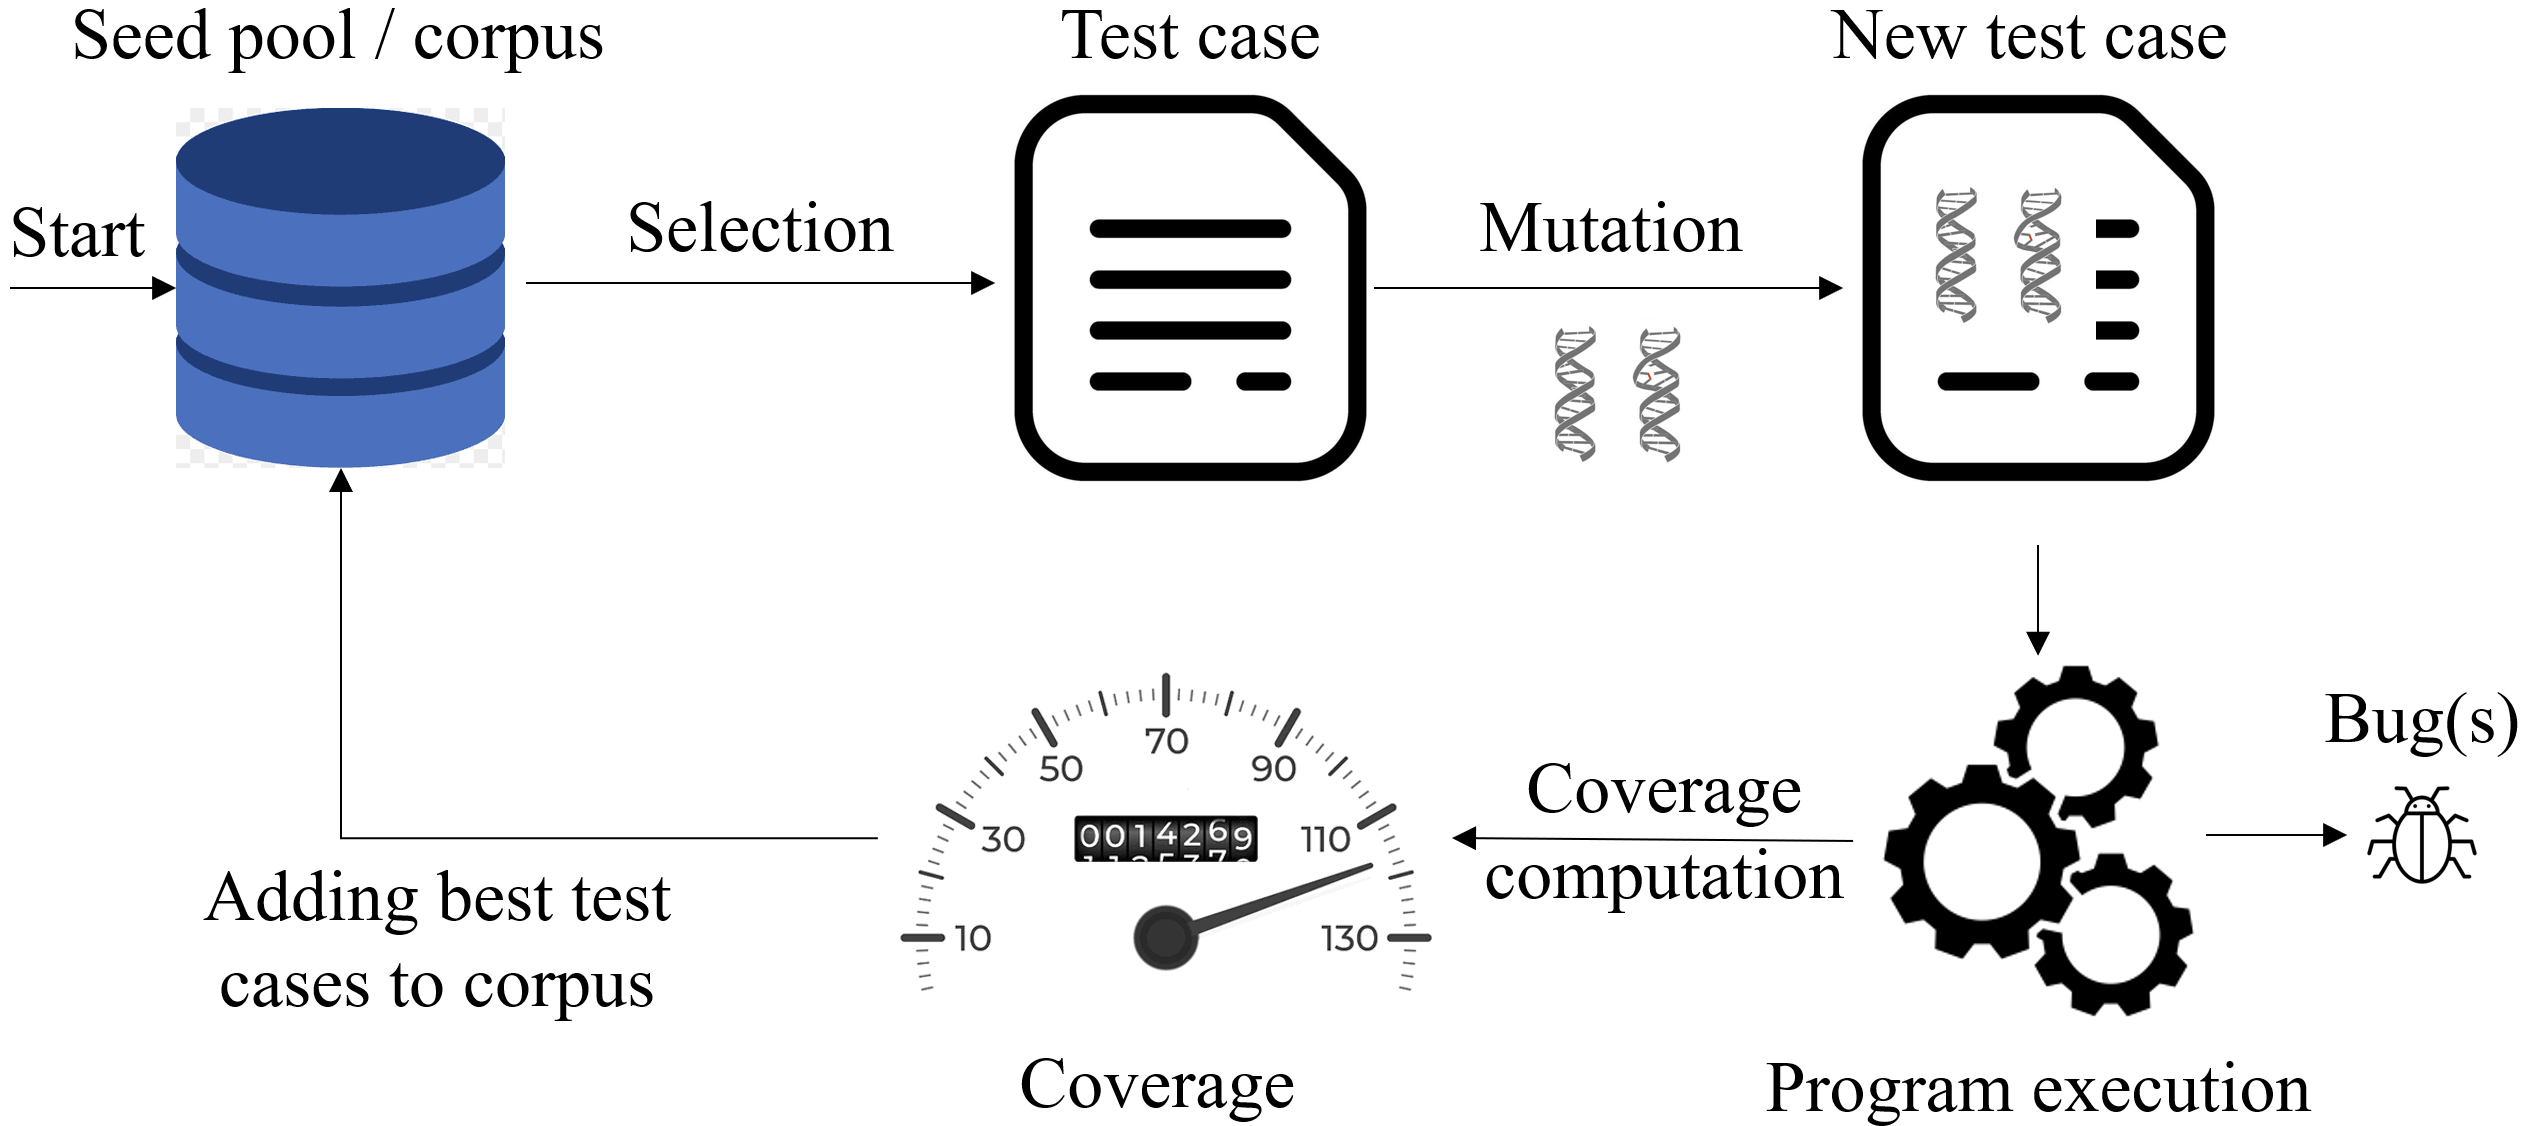
\includegraphics[width=3.25in]{coverage-fuzz.png}
        \vspace{-18pt}
        \caption{Traditional Coverage-Guided Fuzz Testing}
        \label{fig:coverage-fuzz}
    \end{minipage}%
    \begin{minipage}{0.5\textwidth}
        \centering
        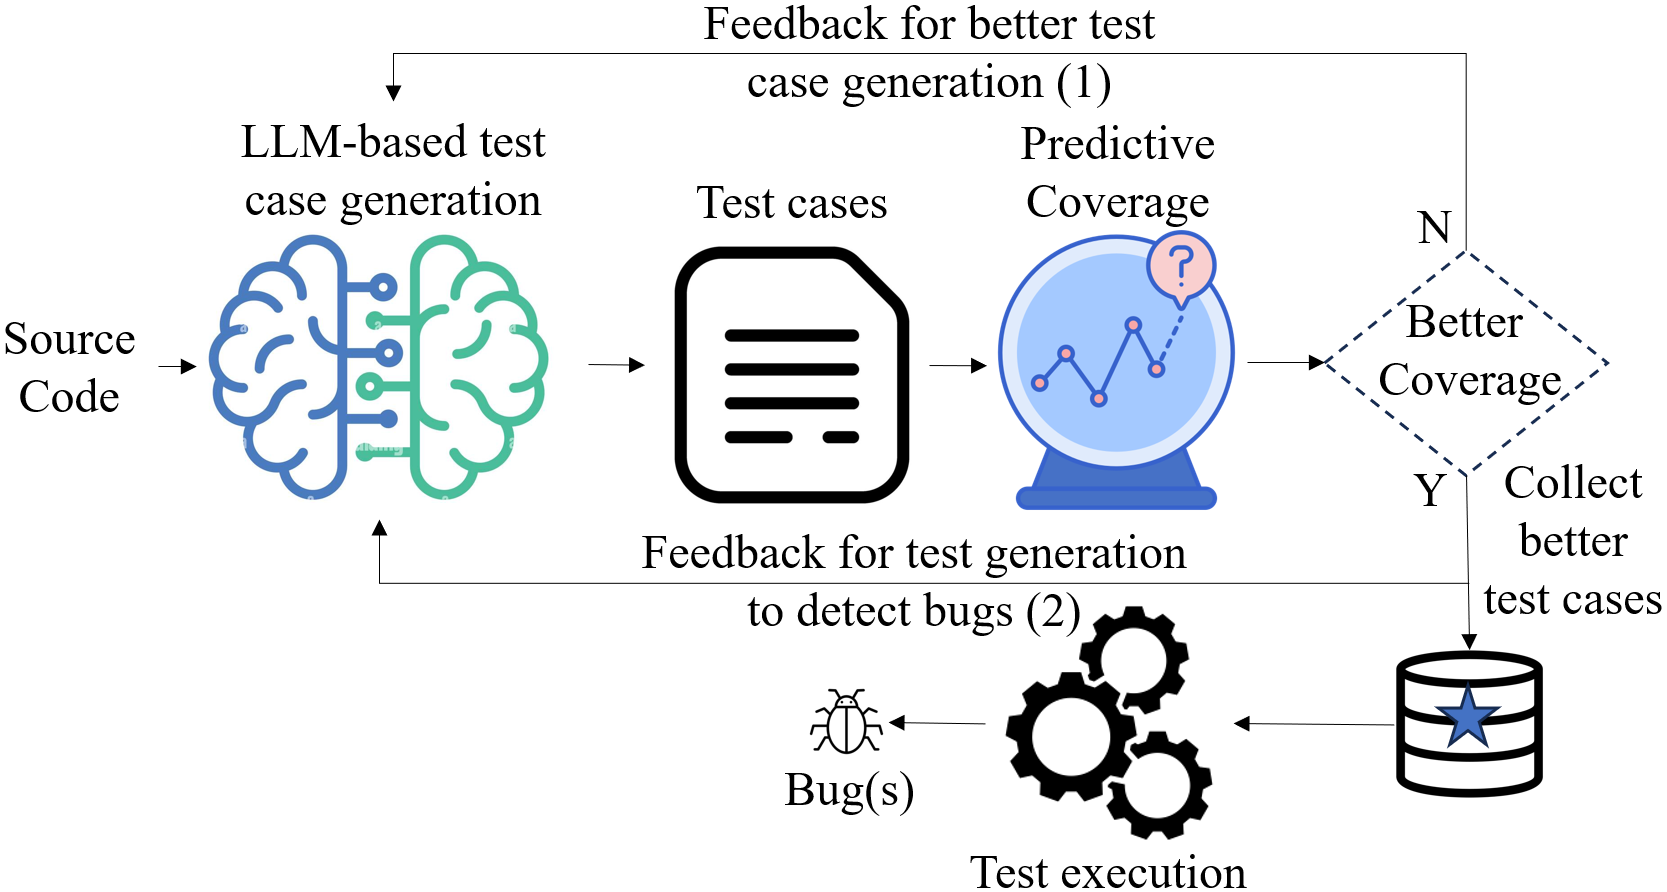
\includegraphics[width=3.3in]{fuzzwise2.png}
        \vspace{-18pt}
        \caption{Predictive Coverage-Guided Intelligent Fuzzing}
        \label{fig:fuzzwise}
    \end{minipage}
\end{figure}

%\begin{figure}[t]
%\begin{center}
%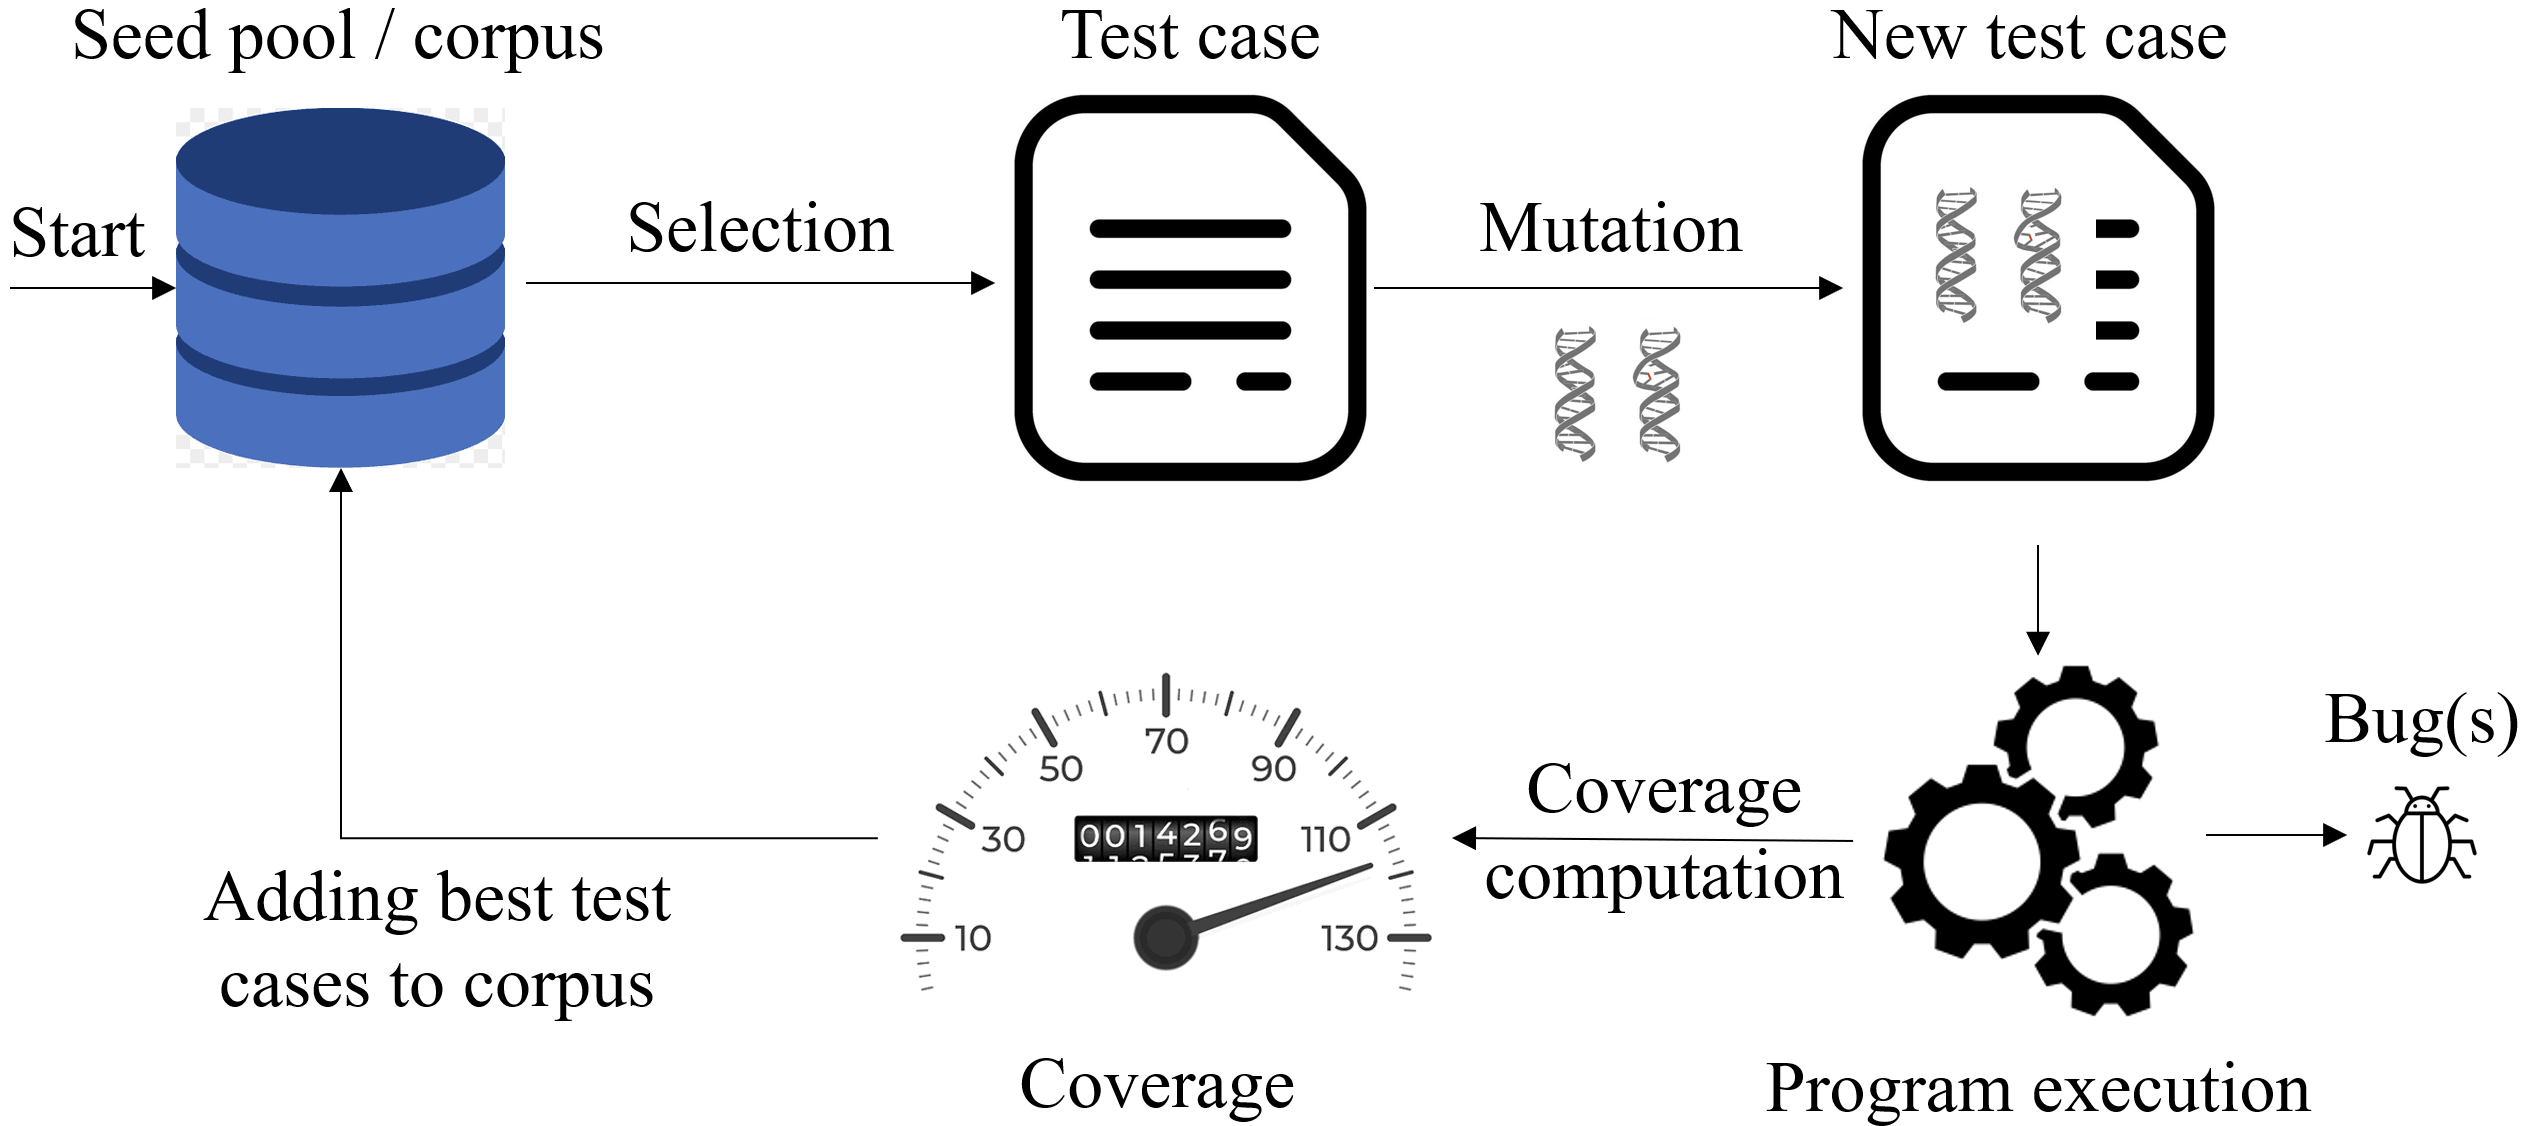
\includegraphics[width=3.4in]{coverage-fuzz.png}
%\vspace{-6pt}  
%\caption{Predictive Coverage-Guided Intelligent Fuzzing Framework}
%\label{fig:coverage-fuzz}
%\end{center}
%\end{figure}

%\begin{figure}[t]
%\begin{center}
%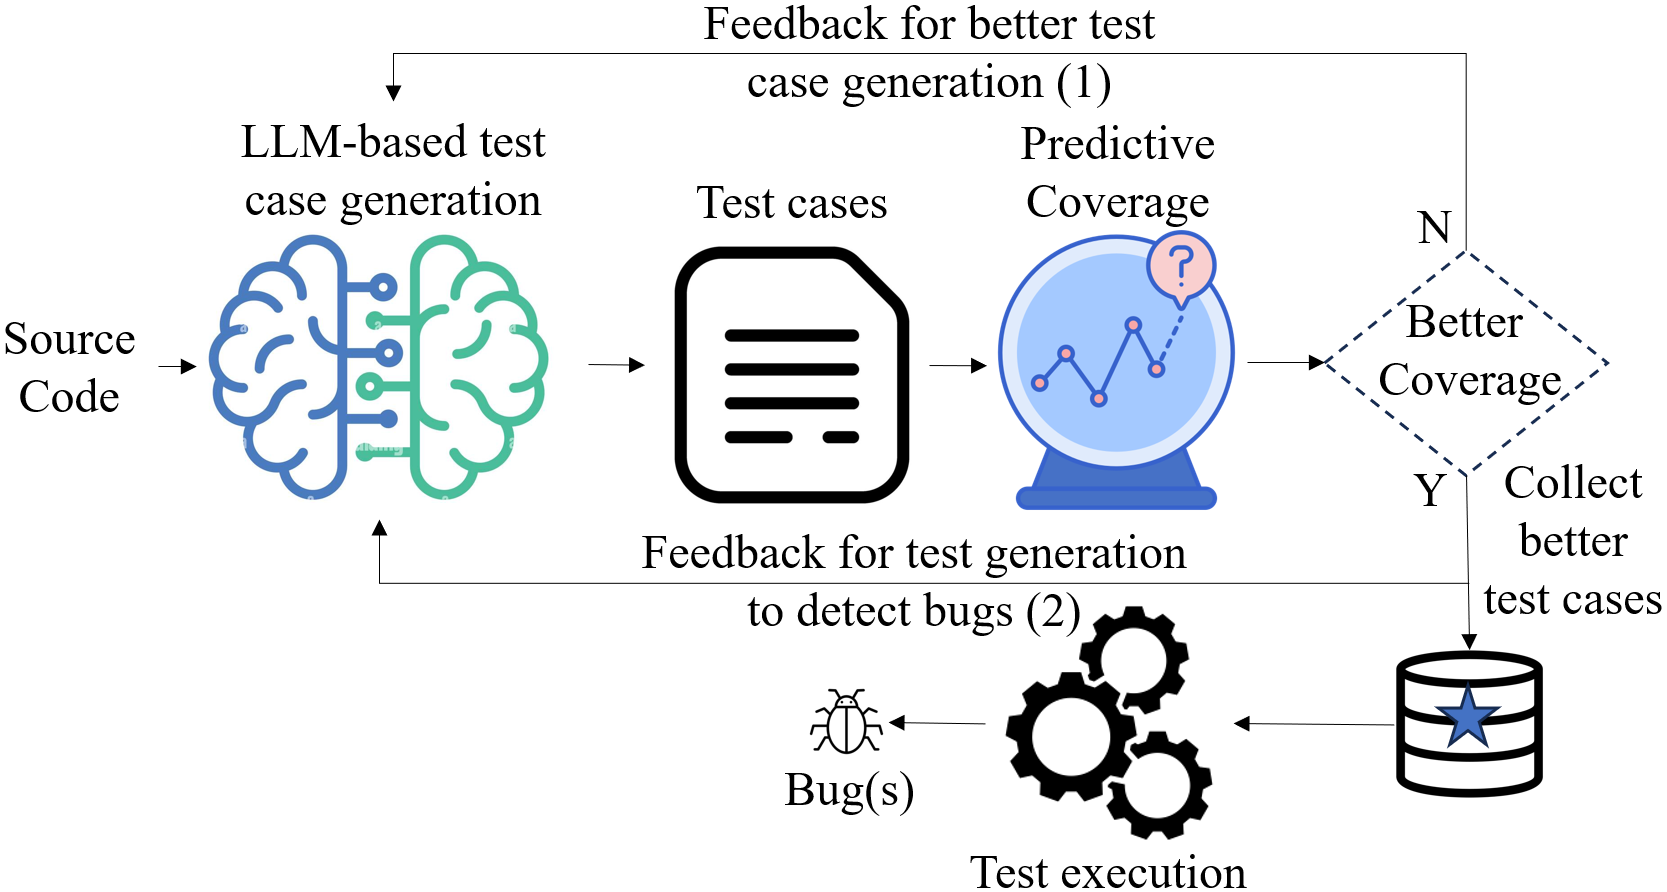
\includegraphics[width=3.5in]{fuzzwise2.png}
%\vspace{-15pt}
%\caption{Predictive Coverage-Guided Fuzzing Framework}
%\label{fig:fuzzwise}
%\end{center}
%\end{figure}

\subsection{Predictive Coverage-Guided Fuzzing Framework}

In this work, we propose {\tool}, a predictive code coverage-guided
intelligent fuzzing framework without actual test execution
(Figure~\ref{fig:fuzzwise}). For an upfront test quality assessment,
our \underline{first idea} is to develop a Large Language Model (LLM)-based code
coverage prediction approach, CodePilot~\cite{forge24}, that estimates
the quality of the generated test cases with regard to their code
coverages. The preliminary work on code coverage prediction is
described in~\cite{forge24}. This predictive approach aims to
identify, prioritize, and execute only the test cases that are likely
to contribute to higher total code coverage, thereby conserving
computational resources in actual execution, and focusing testing time
on the areas that likely need further testing.

Our \underline{second fundamental concept} aims to tackle the challenges
associated with mutations and the seed corpus. Instead of relying on
the conventional approach of mutating tests and enhancing the seed
corpus, we propose leveraging a LLM to automatically generate test
cases for the given source code under test. Within {\tool}, the
feedback loop is activated subsequent to the prediction of code
coverage. Once our predictive code coverage module determines that a
generated test case does not contribute to a higher total coverage of
the current test suite, we reintroduce these cases to the LLM.
This process enhances the generation of test cases from the LLM with
the goal of covering more un-tested areas in subsequent cycles. This
is carried out in the feedback loop (1) (Figure~\ref{fig:fuzzwise}).

Once predictive code coverage module determines that~a generated
test case would contribute to achieving higher overall coverage, we
collect it into the current test suite. However, we defer their
execution at this stage. Instead, the framework proceeds to the second
loop (2), where it prompts the LLM to generate additional test cases
with the main goal of enhancing the probabilities of detecting bugs and
runtime errors.

To enhance both effectiveness and efficiency, we instruct the LLM to
generate multiple test cases simultaneously: one seed test case and
several ``close'' variants. This approach aims to exploit a
faulty area within the source code by producing test cases closely
related to the seed. As the second loop (2) starts, we
expect that the LLM will begin exploring a new faulty area in the
source code. This functionality mirrors the traditional approach of
using different seed test cases. By adopting this strategy, we aim to
address the ``plateau'' issue, where the fuzzing process becomes
stagnant despite generating numerous mutations. The process will
terminate once either the cumulative code coverage of the entire test
suite reaches 100\% or the predetermined time limit is reached.


%We have conducted several experiments to evaluate {\tool}. Our result
%in the FixEval dataset~\cite{haque2023fixeval} shows that within a
%time limit, {\tool} generates significantly less test cases (only
%about 0.0065\%), yet to detect more runtime errors than the
%conventional fuzz testing framework in Jazzer~\cite{jazzer}. {\tool}
%is more efficient in runtime error detection compared to the baseline:
%on average, {\tool} executed {\bf 163} generated test cases to detect a
%runtime error, while Jazzer executed {\bf 4,217,067} test cases per error,
%thus showing that {\tool} saves execution time over Jazzer for
%ineffective test cases. The ratio between the number of effective test
%cases over the total number of generated ones for {\tool} ({\bf 0.48})
%is also higher than that of Jazzer ({\bf 0.41}), showing that {\tool}
%produces more effective, higher-quality test cases. Our result also
%shows that it took significantly less number of test cases for {\tool}
%to detect the next runtime error from the previous one than Jazzer.
%Moreover, we show that {\tool} overcomes the coverage plateau better
%than Jazzer. Importantly, the code coverage prediction module is
%sufficiently accurate in which {\bf 67\%} of test cases predicted by
%{\tool} as enhancing the coverage are indeed effective in doing so.

%The key contributions of this paper include:

%{\bf 1. {\tool}:} a novel predictive code coverage-guided fuzz testing
%framework that leverages predictive code coverage to conserve
%computational resouces in execution.

%{\bf 2. LLM-based Test Case Generation:} we leverage LLM to analyze the
%given code and generates the test cases with the feedback loops to
%iteratively improves the test case quality.

%{\bf 3. Extensive Empirical Evaluation:} to demonstrate that {\tool} is
%more effective and efficient than the baseline fuzzing models. Data
%and code is available at~\cite{fuzzwise-website}.









\subsection{Research Objectives and Anticipated Results}

%\begin{wrapfigure}{l}{0.62\textwidth}
%\begin{figure}[t]
%    \centering
%    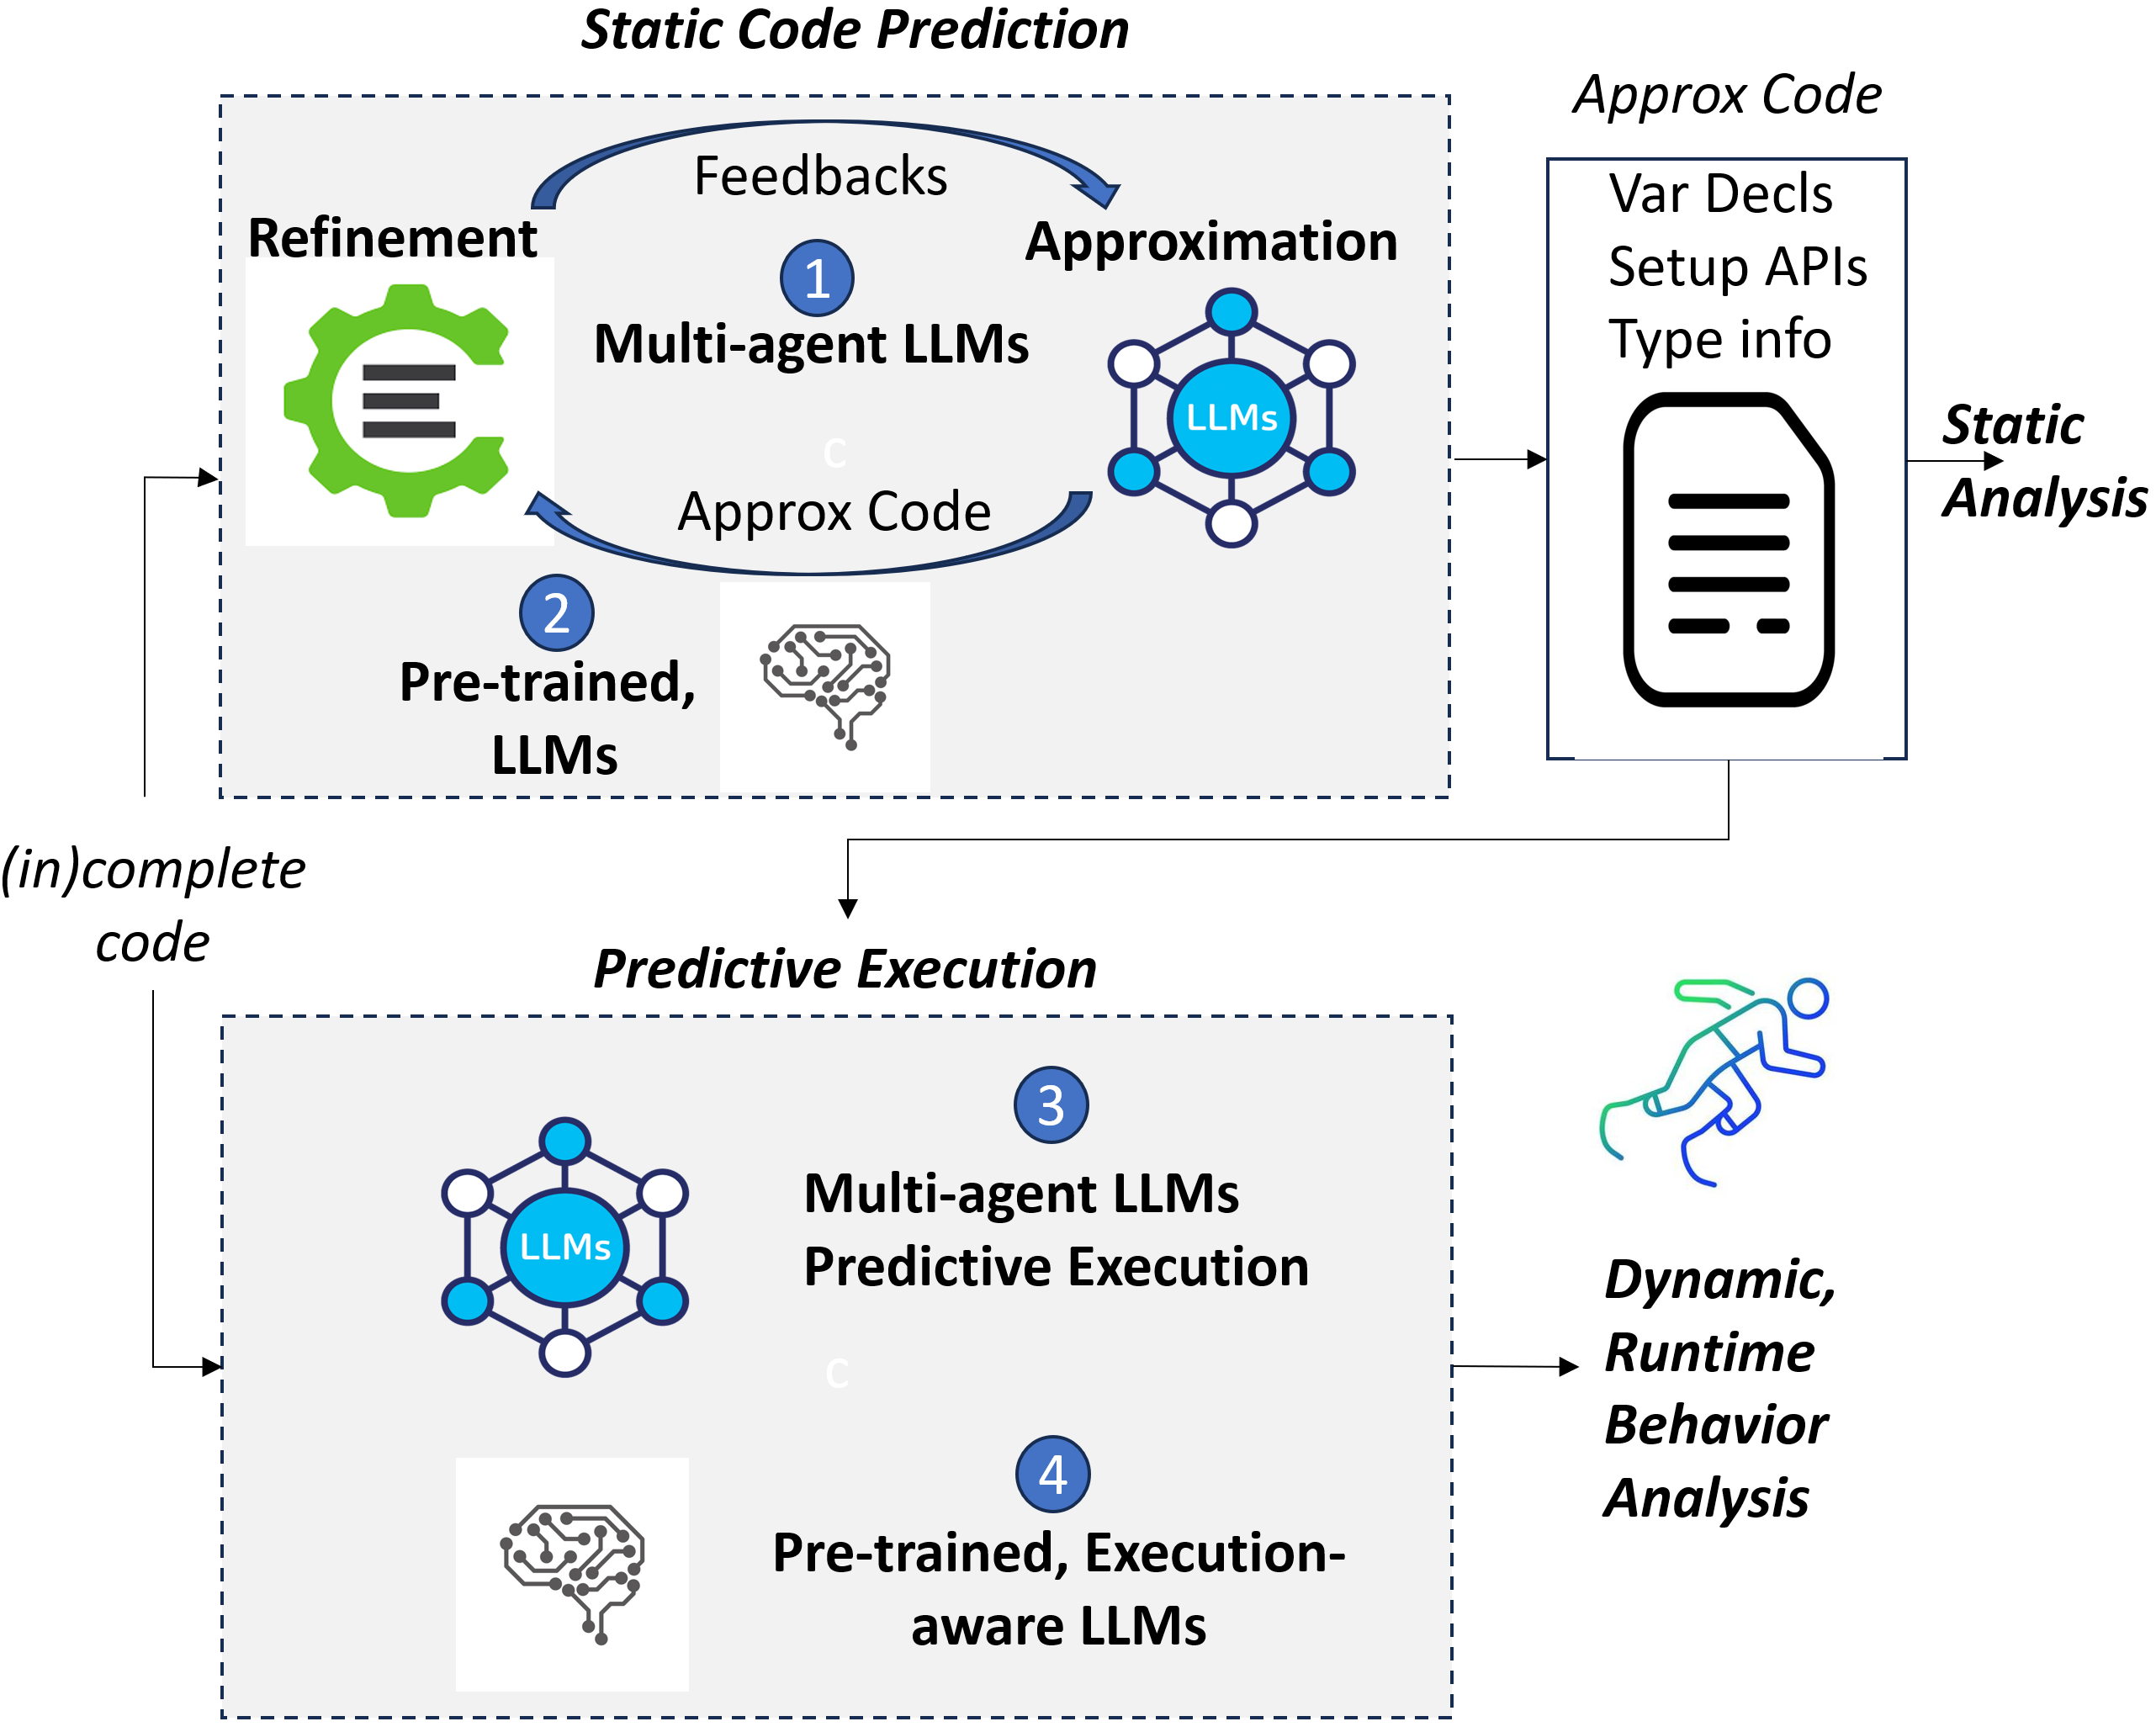
\includegraphics[width=0.62\textwidth]{overview-new.png}
%    \vspace{-10pt}
%    \caption{Predictive Program Analysis: Analyzing Dynamic Program Behaviors}
%    \label{fig:arch}
%\end{wrapfigure}


We seek to advance the state-of-the-art in fuzz testing by means of
{\tool}, a {\bf Predictive Coverage-Guided Intelligent Fuzzing}
framework, with the goal of overcoming the issues listed in the
introduction. We aim to establish {\em a scientific foundation, novel
  methodologies, frameworks, models, and algorithmic solutions for
  predictive coverage-guided fuzz testing} with the following focus
areas:



(1) Large Language Models (LLM)-based {\bf predictive code coverage} (without test execution),

(2) LLM-based, targeting, {\bf test case generation}, and

(3) {\bf predictive coverage-guided fuzz testing} with LLMs.

%\noindent Figure~\ref{fig:arch} illustrates the framework for {\tool},
%which will allow the construction of efficient program analysis
%techniques for (partial) code, also based on which downstream vulnerability detection and assessment applications can be built.

Our predictive program analysis framework is also beneficial in other
scenarios in addition to programming assistants for incomplete code in
an IDE. Predictive execution is not aimed to replace actual
execution. Rather, it offers a solution where the actual execution is
impossible, specifically in the scenarios 1) where the complete source
code is not available, or 2) where the analysis or approximation on
the behavior of the code is needed/desired without actual execution
and some degree of inaccuracy in prediction is tolerable.  First, the
first scenario can be exhibited in several examples, e.g., in the code
snippets in Stack Overflow or GitHub gist. They often miss contextual
information, such as imports and definitions of variables and
functions. It can take a great deal of efforts to integrate such code
snippets to a codebase.
%Horton and Parnin~\cite{horton2018gistable} reported that ``75.6\% of
%Python code snippets in gist require non-trivial configuration to
%overcome missing dependencies, configuration files, reliance on a
%specific operating system, or some other environment
%configuration''. Hossain {\em et al}~\cite{hossain2019executability}
%found that after installing the top 40~Python packages, the overall
%execution success rate for Stack Overflow Python code snippets is only
%27.9\% considering those running in either Python 2 or Python 3
%environments.
%Moreover, in~his keynote,
%Yahav~\cite{yahav2023fse} poses a need to approximate the execution of
%the incomplete code under editing in an AI-assisted programming
%environment.
Second, the instances of the second scenario can include the
analysis/approximation~of the behavior to check properties of
untrusted code or~to~detect bugs early. Moreover, even with complete
code, setting~up running environments for dynamic analysis is
undesired due to missing third-party dependencies and complex build
configurations.

The \underline{key philosophy} that drives our work is that the analysis of
partial code can be learned from the analysis of entire programs in
the wealth of information obtained from ultra-large-scale, open-source
software repositories. To accomplish these tasks, we propose the
following thrusts of research in {\tool} (Figure~\ref{fig:arch}):

\noindent \textbf{Thrust 1. LLM Multi-agents and Pre-trained Language Models for Static Analysis on Incomplete Code.} ({\em Section~\ref{sec:thrust1}})
As depicted in Figure~\ref{fig:pre-rec}, conventional Program Analysis
(PA) techniques exhibit high precision and recall when applied to
complete code. However, when dealing with incomplete code, these
techniques may experience a significant decrease in recall due to
missing information, despite maintaining reasonably high precision or
experiencing a slight decrease in precision due to their strict and/or
heuristic analysis rules (denoted by PA $\medblacklozenge$ in
Figure~\ref{fig:pre-rec}). On the other hand, employing an LLM directly
for downstream analysis tasks may yield higher recall, thanks to the
LLM's ability to explore the solution space (denoted by LLM
$\circledast$ in Figure~\ref{fig:pre-rec}). However, the precision of
  LLM analysis on incomplete code tends to be lower compared to
  conventional PA tools due to the lack of ability in specific
  analysis in the downstream tasks.

We propose a tandem solution that combines LLMs and PA agents to
leverage the strengths of both methodologies. We aim to harnessing the
complementary capabilities of LLMs and PA: {\em LLMs' expansive search
  capabilities} and {\em PA-based agents' semantic verification
  abilities}.
%This integrated approach aims to optimize performance by
%harnessing the complementary capabilities of LLMs and PA
%techniques.

We advocate for a novel paradigm, called {\bf predictive program
  analysis}, which operates on the principles of {\em
  Approximation-Refinement} for Analysis. In the Approximation phase,
a large language model (LLM) acts as a machine learning (ML) agent to
fill in missing information within incomplete code. The missing
information that will be filled by the LLM could be manifested {\em
  explicitly}, e.g., in terms of missing variable declarations, setup
API method calls, import statements, and exception handling types, or
{\em implicitly}, e.g., in terms of missing type information of 
program elements, missing dependencies, etc.

%Leveraging an LLM for this is advantageous due to its capability of code understanding.

\begin{wrapfigure}{l}{0.55\textwidth}
    \centering
    \begin{tikzpicture}
        \pgfplotsset{width=3in,
         }
        \begin{axis}[
            scale=1,
            view={20}{35},
            ticklabel style={font=\footnotesize},
            xlabel={\normalsize \textbf{Precision} ($\rightarrow$)},
            ylabel={\normalsize \textbf{Recall} ($\rightarrow$)},
%            zlabel={\normalsize \textbf{Source Code} ($\rightarrow$)},
            xlabel style={rotate=-10, yshift=0.1cm},
            ylabel style={yshift=0.5cm, xshift=0.225cm,rotate=65},
            zlabel style={yshift=-0.2cm, xshift=-0.5cm,rotate=0},
            xmin=0, xmax=4,
            xtick={1,2,3},
            ymin=0, ymax=4,
            ytick={1,2,3},
            zmin=0, zmax=1,
            ztick={0,1},
            xticklabels={\textit{Low},\textit{Medium},\textit{High}}, % Set custom x-tick labels
            yticklabels={\textit{Low},\textit{Medium},\textit{High}}, % Set custom y-tick labels
            zticklabels={\textit{Partial Code},\textit{Complete Code}},
            ztick pos = left,
            xticklabel style={rotate=0},
            yticklabel style={rotate=0, yshift=0.325cm},
            zticklabel style={yshift=0.4cm},
            % Set custom z-tick labels
            axis background/.style={fill=gray!10},
            xmajorgrids=true,
            ymajorgrids=true,
            zmajorgrids=true,
            grid style={dotted, thick},
            axis equal,
            visualization depends on={value \thisrow{m} \as \labela},
        ]
        % Add a node at x=High, y=High, z=Complete
        \draw[dashed,black,thick] (axis cs:3,3,1) -- (axis cs:0,3,1) node[midway, right] {};
        \draw[dashed,black,thick] (axis cs:3,3,1) -- (axis cs:3,4,1) node[midway, below] {};
        \draw[dashed,black,thick] (axis cs:3,3,1) -- (axis cs:3,3,-0.2);
        \node[above right] at (axis cs:{2.9,2.55,1}) {\textcolor{blue}{\large $\medblacklozenge$}};

        % Thick axes
        \draw[black, thick] (axis cs:0,4,-0.3) -- (axis cs:4,4,-0.3) node[midway, right] {};
        \draw[black, thick] (axis cs:0,4,-0.3) -- (axis cs:0,0,-0.3) node[midway, right] {};
        \draw[black, thick] (axis cs:0,4,-0.3) -- (axis cs:0,4,1.3) node[midway, right] {};
        

        % Add points.
        \node[above right] at (axis cs:{3,0.75,0}) {\textcolor{red}{\large $\medblacklozenge$}};
        \node[above right] at (axis cs:{2.95,1.85,0}) {{\textcolor{meatbrown}{\small $\bigstar$}}};
        \node[above right] at (axis cs:{2.55,1.5,0}) {\textcolor{red}{{\small $\circledast$}}};

        % % Add Origin
        % \node[above right] at (axis cs:{4,-0.2,0}) { $\circ$};

        % Add optimal point
        \node[above right] at (axis cs:{3.08,2.3,0}) { \textcolor{dkgreen}{{\footnotesize $\circ$}}};

        \end{axis}
        \draw[gray,line width=0.5pt,rotate=15,fill=red,opacity=0.125] (3.75,0.85,0) circle (1.75 and 0.85);

        % Add node labels
        \node[text width=2cm] at (6,3.75,1) 
            {\footnotesize{\textcolor{blue}{PA}}};
        \node[text width=2cm] at (5.0,1.275,0) 
            {\footnotesize{\textcolor{red}{PA}}};
        \node[text width=2cm] at (4,2.025,0) 
            {\footnotesize{\textcolor{red}{LLM+PA}}};
         \node[text width=2cm] at (3.875,1.7,0) 
            {\footnotesize{\textcolor{red}{LLM}}};
    \end{tikzpicture}
    \vspace{-20pt}
    \caption{Efficacy of various \textcolor{red}{\textit{\textbf{partial}}} and \textcolor{blue}{\textit{\textbf{complete}}} program analysis approaches, with ({\small $\medblacklozenge$}), and without ({\footnotesize $\circledast$}, {\footnotesize $\bigstar$}) learning-based knowledge.}
    \label{fig:pre-rec}
\end{wrapfigure}


A naive solution is to take whatever information the LLMs completed
and feed to a traditional program analysis as is. However,
researchers have shown that while LLMs are remarkable in code
generation with correct syntaxes, the produced code often contains
semantic errors and even do not compilable.  Thus, the Refinement
phase employs a program analysis (PA)-based agent to verify the
completed code output by the LLM. This PA-based agent utilizes the
compiler technology to ensure that the generated code is compilable
and consistent with used external libraries. The iterative interplay
between the LLM-based agent and the PA-based agent continues until a
compilable code is achieved.
%If after a specified number of iterations the code remains
%uncompilable, human intervention may be sought for final resolution.
In brief, the interplay between LLM and PA agents has two objectives:
1) to enhance recall compared to the PA-only solution (via the
Approximation of the incomplete code), and 2) to
maintain or even improve precision beyond what can be achieved with
LLM-only solution by integrating PA to ``correct'' the LLM's solution
(via the result Refinement).
%{\em Such interplay between the LLM and PA agents aims to enhance both the
%recall and precision} of the analysis when comparing with the approach
%using directly the PA technique on the incomplete code.

%The LLM is used to expand the candidate list of potential complete
%code for the current incomplete snippet, and PA is used to verify to
%make sure the validity of the chosen candidate. Subsequently,
%downstream program analysis techniques can be applied in the Analysis
%phase.
%It's important to acknowledge that the LLM may not always be capable
%of providing the exact missing information that developers would
%create when incorporating incomplete code snippets into their projects
%because each project might have its own . However, leveraging its
%proficiency in understanding code, we anticipate that it will fill in
%the gaps with the most probable information for the given incomplete
%code. Subsequently, following verification by the PA agent, the code
%is rendered complete and ready for analysis techniques to generate
%more accurate results in which without our framework, these techniques
%would be ineffective in handling incomplete code.







%One of the key foundations of {\tool} lies in its neural structural analysis component, which is built upon the well-defined structure and semantics of source code. This component serves two primary functions. Firstly, it draws upon the syntactic structures of comprehensive code samples from large-scale repositories in the training dataset. From this data, it constructs an abstract syntax tree (AST) that best encapsulates the syntactic arrangement of the provided partial code, aiming for the highest likelihood or probability. In contrast, existing program-analysis-based partial parsing methods~\cite{ppa08} rely on heuristics derived from the syntactic rules of programming languages, lacking the capacity to rank or score potential candidates. The second task of this component involves labeling code tokens with the corresponding types of syntactic units, encompassing statement types (\code{if}, \code{for}, etc.), variables, fields, methods, classes, and more. Both tasks can be efficiently executed through our dual-learning-based approaches.

%Source code has a well-defined structure and semantics. Thus, the basic infrastructure in {\tool} is the neural structural analysis component, which primarily has two tasks. First, it learns from the syntactic structures of the complete code in the training dataset collected from large-scale code repositories, to derive the abstract syntax tree (AST) that best represents the syntactic structure of the given partial code, i.e., with the highest likelihood/probability. The existing program-analysis-based partial parsing approaches~\cite{ppa08} rely on the heuristics on the syntactic rules of the programming languages. They do not give us any ranking or scores among the potential candidates. The second task of this component is to tag the code tokens with the types of the syntactic units including the statement types (\code{if}, \code{for}, etc.), variables, fields, methods, classes, etc. Both of the tasks can be performed with our learning-based approaches in a dual-learning manner.
  
%\vspace{3pt}
%\noindent \textbf{Thrust 2. Pre-trained Large Language Models for
%  Incomplete Code Static Analysis} ({\em Section~\ref{sec:thrust2}})
%Our work is driven by the fundamental belief that insights gained from
%training by complete programs within vast repositories of
%ultra-large-scale, open-source software can inform the analysis of
%partial code.

While exploring LLM-based multi-agent solution, we also aim to develop
smaller models via pre-trained language models. Our work is driven by
the fundamental belief that insights gained from training by complete
programs within vast repositories of ultra-large-scale, open-source
software can inform the analysis of partial code~\cite{naturalness-icse12}.
%Hindle {\em et al.}~\cite{naturalness-icse12} have shown that code has
%high repetitiveness and predictability and can be captured well by
%statistical models.
Thus, we expect to build/fine-tune pre-trained LLM models to learn
from those repositories.



%The basis components for several analysis techniques on the semantics
%of the program could tentatively include the following (more
%components will be added as the project evolves):

%1) the identification of the APIs of the external libraries in the
%external references in the partial code: this is needed because the
%partial code contains the undeclared reference and/or
%declaration/reference ambiguity without explicit declaration of the
%APIs in the external libraries. The knowledge on the external
%libraries enables more precise analysis of the code snippets.

%2) the inference of the type information for the entities in the
%partial code: due to the ambiguity in the declaration, the types of
%the variables and statements are not always obviously
%identified. Thus, the type inference is a basic service within
%{\tool}.

%3) the inference of the program dependencies among the statements in
%the partial code: several program analysis techniques are based on the
%program dependencies, which are not always obtainable due to the
%incompleteness of the given code fragment.

%4) Program slicing: program slices are important in both code
%understanding and program analysis for code snippets. That allows the
%analysis on the statements affecting or to be affected by a specified
%variable. All traditional program slicing techniques require the code
%to be complete.

\vspace{3pt}
\noindent \textbf{Thrust 2. LLM Multi-agents and Pre-trained
  Language Models for Predictive Execution.}  ({\em
  Section~\ref{sec:thrust2}})

We advocate for an execution paradigm called predictive execution. In
predictive execution, with a specific input, the execution is not
carried out with the computer performing the instruction in the
program. Instead, a trained machine learning model predicts the
execution steps and as a result, the execution trace corresponding to
the input is derived without actual execution.

By simulating program behaviors and outcomes without running the code,
these approaches provide valuable insights into the program's
potential runtime characteristics. Here are some benefits of
predictive execution. First, early error detection: predicting program
executions allows for the early detection of errors and potential
vulnerabilities before executing the code. By simulating different
execution paths and scenarios, predictive execution can enable the
dynamic analysis tools to identify potential issues such as null
pointer dereferences, memory leaks, or buffer overflows without the
need to execute the code in a real-world environment. This early error
detection helps developers catch and fix bugs more efficiently,
reducing the likelihood of critical issues in production. Second,
dynamic analysis techniques that predict program executions play a
crucial role in security analysis. By simulating potential attack
scenarios and analyzing how the program behaves under different
conditions, these tools can identify security vulnerabilities such as
injection attacks, privilege escalation, or data breaches. Predictive
execution helps security professionals assess the resilience
of systems against various threats and vulnerabilities,
enabling proactive security measures and robust defenses. Finally,
predicting executions provides developers with a deeper understanding
of their code's behavior without the need for actual execution. By
simulating program flows and interactions, tools can uncover hidden
dependencies, identify unexpected behaviors, and reveal complex
program dynamics.

%This insight into program behavior helps developers better comprehend their code, debug more effectively, and make informed design decisions.

In addition multi-agent solutions, we also explore the
pre-training language models. We aim to teach a smaller model to analyze
the runtime behaviors via the learning from complete programs in execution.


%Symbolic execution is a means of analyzing a program to determine what
%inputs cause each part of a program to execute. Symbolic execution
%performs executing a program abstractly, so that one abstract
%execution covers multiple possible inputs, which are assumed to have
%symbolic values. We aim to explore the novel area in AI named
%neuro-symbolic learning, which seeks to combine traditional
%rules-based AI approaches with modern deep learning techniques.  We
%will leverage traditional program analysis rules to enhance the
%learning of the characteristics on the execution of the partial code
%fragment.

\vspace{3pt}
\noindent \textbf{Thrust 3. Programming Assistant Applications with Predictive Program Analysis.}  ({\em Section~\ref{sec:thrust3}})


Our last thrust of research is aimed to demonstrate the usefulness of
our solution in different programming assistant applications: 1)
vulnerability detection, 2) dynamic slicing,  etc.

%and 3) debugging and error detection.



%2) fault localization, and 3) code completion.

%\vspace{3pt}
%\noindent \textbf{Thrust ???. Neural Execution Analysis Infrastructure.}
%({\em Section~\ref{}}) All the dynamic analysis techniques require the
%analysis and understanding of the execution. However, for an
%incomplete code, we first need to design a component that can wrap
%around the given code fragment with the minimum code so that the code
%fragment can be executed. When the code is executed, we also need the
%approaches that represent the executed statements and their relations,
%model the execution and stack traces, and model the code coverages
%for an execution.




%Toward this theme, in our preliminary work, we developed DeepPDA
%(Section~\ref{sec:deeppda}), a neural network-based partial program
%dependence analysis approach that learns to derive the program
%dependencies for any code fragments (i.e., both complete and
%incomplete). In our preliminary empirical evaluation, we intrinsically
%evaluated it on Java and C/C++ programs. We trained DeepPDA on
%complete code. For testing, we treated each method individually and
%chose a consecutive portion within the method to predict the program
%dependencies, and compared them against the actual
%dependencies. Overall, DeepPDA predicts CFGs/PDGs in Java with
%an F-score of 94.29\%, and in C++ with an F-score of 92.46\%. As
%another preliminary work (Section~\ref{sec:statype}), we also
%developed an approach to derive the data types of the variables in the
%code snippets. We treat the problem as statistical machine translation
%from source code with partially qualified names to source code with
%full names. Our preliminary evaluation on StackOverflow posts shows
%that our technique achieves high accuracy with 97.6\% precision and
%96.7\% recall in deriving data types in code snippets.

%We also test the usefulness of the PDGs predicted by DeepPDA (i.e.,
%PDG*) on the downstream task of method-level vulnerability
%detection. We discover that the performance of the vulnerability
%detection tool utilizing PDG* is only 1.1\% less than that utilizing
%the PDGs generated by a program analysis tool.
%We also report the detection of 14 real-world vulnerable code snippets
%from StackOverflow by a learning-based vulnerability detection
%tool that employs the PDGs predicted by DeepPDA for these code snippets.

\begin{table*}[t]
	\vspace{-15pt}
\begin{center}
{\footnotesize{
\begin{tabular}{cc}
\begin{tabular}[t]{|p{0.2in}|p{2.95in}|} 
\hline
\multicolumn{2}{|>{\columncolor[gray]{0}}c|}{\textcolor{white}
{\bf Year 1 Project Milestones \& Deliverables}}\\
\hline 
\hline
\multicolumn{2}{|c|}{\bf T1. LLM Multi-agents for Static Analysis}\\
\hline
{\bf 1.1} & LLM Multi-agent framework\\
{\bf 1.2} & LLM Multi-agent and Static Analysis\\
{\bf 1.3} & Pre-trained Language Models for Static Analysis\\
\hline
\hline
\multicolumn{2}{|c|}{\bf T1. Pre-trained Language Models for Static Analysis}\\ 
\hline
{\bf 1.4} & Pre-trained Language Models for Static Analysis\\
\hline
%\hline
%\multicolumn{2}{|c|}{\bf Integrate Code Synthesis into Tools}\\
%\hline
%{\bf 1.5} & \goalOneFour.\\
%\hline
\multicolumn{2}{c}{}
\end{tabular}
&
\begin{tabular}[t]{|p{0.2in}|p{2.95in}|} \hline
\multicolumn{2}{|>{\columncolor[gray]{0}}c|}{\textcolor{white}
{\bf Year 2 Project Milestones \& Deliverables}}\\
\hline 
\hline
\multicolumn{2}{|c|}{\bf T2. LLM Multi-agents for Predictive Execution}\\
\hline
{\bf 2.1} & LLM Multi-agents with Graphs\\
{\bf 2.2} & LLM Multi-agents with Execution\\
%{\bf 2.3} & Integrate Evaluation Framework into Design Environment\\
%{\bf 2.4} & Evaluate CRL Framework with Existing Models\\
%{\bf 2.3} & \goalTwoThree.\\

\hline
\hline
\multicolumn{2}{|c|}{\bf T2. Pre-trained Language Models for Predictive Execution}\\ 
\hline
%{\bf 3.1} & Design New Code Representations and Learning Models.\\
{\bf 2.3} &  Pre-trained Language Models for Predictive Execution\\
%{\bf 2.4} & Advance FL and RT-CI Approaches.\\
%{\bf 2.5} & Advance Regression Testing in CI Approaches.\\
%{\bf 2.5} & Advance APR Approaches with Framework.\\
\hline
%\hline
%\multicolumn{2}{|c|}{\bf Community Involvement: Capacity Building}\\
%\hline
%{\bf 2.4} & \goalTwoFour.\\
%{\bf 2.5} & \goalTwoFive.\\
%{\bf 2.6} & \goalTwoSix.\\
%\hline
\multicolumn{2}{c}{}
\end{tabular}
\end{tabular}\\
\vspace*{-.3cm}
\begin{tabular}{c}\hline
\multicolumn{1}{|>{\centering\columncolor[gray]{0}}p{6.44in}|}{\textcolor{white}
{\bf Year 3 Project Milestones \& Deliverables}}\\
\hline
\end{tabular}\\
\vspace*{-.2cm}
\begin{tabular}{cc}
\begin{tabular}[t]{|p{0.2in}|p{2.95in}|}
\hline
\multicolumn{2}{|c|}{\bf T3. Programming Assistant with Predictive Analysis}\\
\hline
{\bf 3.1} & Dependency Analysis\\
{\bf 3.2} & Debugging and Error Detection\\
\hline
%\hline
%\multicolumn{2}{|c|}{\bf \goalTwo}\\ 
%\hline
%{\bf 3.3} & \goalThreeThree.\\
%\hline
\multicolumn{2}{c}{}
\end{tabular}
&
\begin{tabular}[t]{|p{0.2in}|p{2.95in}|}
\hline
\multicolumn{2}{|c|}{\bf T3. Programming Assistant with Predictive Analysis}\\
\hline
%{\bf 3.1} & Design New Code Representations\\
{\bf 3.3} & Dynamic Slicing\\
\hline
\multicolumn{2}{c}{}
\end{tabular}
\end{tabular}
\vspace{-15pt}
}}
\end{center}
\vspace*{-.3in}
%\caption{Tasks and Milestones. (Rep. = Representation)}
\caption{The 3-year schedule of Thrusts, Tasks, and Milestones of this proposal.}
%the schedule of Thrusts, Tasks, and Milestones of this proposal.
%\vspace{-10pt}
\label{tab:milestones}
\vspace{-10pt}
\end{table*}
%




%\subsection{Significance of This Proposed Project: NSF Merit Criteria}

%\section{Relevance to Secure and Trustworthy Cyberspace}

%This project will develop novel concepts, representations, algorithms,
%models, and tools to support early software vulnerability
%detection. It is transformative and directly help improve software
%quality with novel program analysis-based software security and
%vulnerability detection tools on code snippets.

\section{Intellectual Merits}

%The results of this project will be transformative and directly help
%improve software quality with novel program analysis-based software
%security tools.

\noindent \underline{{\bf Advance the state-of-the-art knowledge and
    understanding}}. Predictive fuzz testing infrastructure in Thrusts
1--3 will advance the body of knowledge and theoretical foundations in
the area of {\bf machine learning and AI for software testing}. They
will also help advance the practical software testing tools.

\noindent \underline{{\bf Scientific foundation, creative/original
    research}}. (1) a novel intelligent framework for fuzz testing,
(2) a new set of code coverage analysis tools, and (3) a new set of
fuzz testing tools.

\section{Broader Impacts}

\underline{{\bf (1) Transformative and benefits to society}}. Our
results will be transformative and directly benefit to our society.
They will lead to increasing developers' productivity, software
quality \& reliability.  Our validation involves students and
professionals, promoting teaching, training, and learning of both {\bf
  software testing} and {\bf machine learning} techniques that have
wide impacts in industry and academic communities.

\noindent\underline{{\bf (2) Foster other related research
    activities}}. Our results will foster {\em research activities in
  related fields of {\bf machine learning} and {\bf software testing}},
and the applications in software testing and reliability.
%We will produce theoretical concepts and techniques that are novel in
%deep learning, e.g., novel neural networks to model and learn for
%code.
%The applications of our neural program analysis in software
%engineering applications will advance software security and
%reliability.

%The collected {\bf large scale bug\&fix corpus} will be useful for
%software quality and reliability research.
%Innovations in CRL could be used to {\bf advance other SE tasks}. We
%will also develop {\bf novel DL-based bug detect-fix} approaches.


\noindent\underline{{\bf (3) Education, dissemination, and broader participation}} (Section~\ref{edu}). The
research will enhance the infrastructure for teaching/research via
tools and data sets for use by students and practitioners, and for
enhancement by researchers. We will provide related learning
modules for educators as well. It will include outreach activities for
undergraduate students, underrepresented groups, minorities, and women
in science.
%contribute novel
%teaching modules to our curriculum.
%Details will be presented in Section~\ref{edu}


\iffalse
\begin{itemize}
	\vspace{-5pt}
\itemsep-0.2em 
  \item {\bf Transformative and benefits to society}. Our 
    results will be transformative and directly benefit to our
    society. 
    They will lead to increasing developers' productivity
    and software quality \& reliability. 
    Our validation involves students and
    professionals, promoting teaching, training, and learning of bug detecting and fixing techniques that have wide impacts 
    in industry and academic communities.

%report

  \item {\bf Foster other research activities}. Our results will
    foster research activities in related fields of deep learning and
    software quality. 
    This project will produce theoretical
    concepts and techniques that are novel even in deep learning, e.g.,
    novel neural networks for modeling and learning code. 
    The collected large scale bug fixing corpus will be useful for software testing and reliability research in general.
    %e.g.,   code transformation. 
%    This project will also advance
%    the state-of-the-art research in large-scale program analysis with
%    deep neural network models.

%The representation for software security vulnerabili will be useful in
%research on software security, malware detection, vulnerability
%reports, and automatic security patching.


  \item {\bf Education, dissemination, and broader participation}.
  The research will enhance the infrastructure for teaching and
  research by providing tools and data sets for use by students and
  practitioners, and for enhancement by other researchers. We will
  provide related learning modules for educators as well. It will
  contribute novel teaching modules to our curriculum. Details will be
  presented in Section~\ref{edu}.

%Details are in Section 4.

\end{itemize}
\fi


\section{Related Work}
%Our project is closely related to the following research literature: 

%The evolution of fuzzing techniques from their inception to the specific application of coverage-guided fuzzing in Java signifies a fascinating journey through the development of software testing methodologies. This progression reflects the growing complexity of software systems and the necessity for more sophisticated tools to ensure their reliability and security. Fuzzing, in its earliest form, entailed providing invalid, unexpected, or random data as input to computer programs, aiming to uncover bugs and vulnerabilities by triggering unusual program paths or error conditions not anticipated by developers. The simplicity of this approach enabled its broad application across various programming languages and platforms, laying the groundwork for more specialized fuzzing techniques.

%This technique leverages instrumentation to gather coverage information, guiding the fuzzer to generate inputs maximizing code coverage. While highly effective in languages like C and C++, where memory corruption vulnerabilities are common, adapting coverage-guided fuzzing to languages such as Java posed new challenges. Java's managed execution environment, bytecode instrumentation complexity, and extensive standard library necessitated novel approaches.

%Tools like JQF (Java QuickCheck Fuzz) {\color{blue}[REF]} and Kelinci {\color{blue}[REF]} have risen to these challenges, offering coverage-guided fuzzing capabilities tailored to Java's unique environment. JQF integrates with property-based testing frameworks, facilitating fuzz testing of Java programs guided by code coverage feedback. These tools typically dynamically instrument bytecode to collect coverage information, enabling the fuzzer to explore uncharted paths and uncover bugs difficult to detect through conventional testing.

%As the fuzzer explores new paths, the number of paths to explore can
%grow exponentially, leading to resource exhaustion and
%inefficiency. This issue becomes more pronounced when fuzzing software
%with deeply nested conditional branches or intricate loops, where the
%number of possible paths can become prohibitively large. The challenge
%of path explosion in large and complex codebases is discussed by

%This limitation can hinder the fuzzer's ability to uncover certain types of bugs, such as race conditions or timing-dependent vulnerabilities.
%Addressing the struggle with non-deterministic software behavior,

%Initially, when a coverage-guided fuzzer begins exploring a software
%application, it rapidly increases code coverage by discovering new
%execution paths and exercising different code branches. However, as
%the fuzzer exhausts high-coverage paths and explores less-covered
%regions of the codebase, it may encounter diminishing returns in
%terms of code coverage improvement. Eventually, the fuzzer reaches a
%point where it finds it challenging to identify new paths to explore,
%leading to stagnation in code coverage growth. However,

%This approach effectively guides the fuzzer into previously underexplored areas of the code, thereby enhancing overall coverage and the likelihood of uncovering hidden vulnerabilities.

%Similarly, Fuzz4All represents a groundbreaking advancement in addressing the coverage plateau problem. Its universal application across multiple programming languages and systems, combined with its utilization of LLMs for input generation, allows Fuzz4All to generate a wide variety of realistic test inputs. This capability enables Fuzz4All to explore new and different features of the input languages, pushing past the limitations of traditional, language-specific fuzzers.

%The tool's innovative use of autoprompting techniques and an LLM-powered fuzzing loop iteratively refines its approach, continuously uncovering new paths and vulnerabilities that would otherwise remain hidden.

%Their success marks a significant step forward in the ongoing development of more effective and efficient fuzzing methodologies, offering new strategies to enhance software reliability and security.

%Both CODAMOSA and Fuzz4All illustrate the potential of integrating
%LLMs with fuzzing techniques to overcome the coverage plateau. By
%producing more diverse and comprehensive test inputs, these tools can
%explore deeper into the software under test, achieving higher
%coverage and revealing bugs that previous fuzzing efforts may have
%missed.

{\bf Fuzzing testing}:
%techniques have been extensively studied in software testing.
Miller {\em et al.}~\cite{miller1995fuzz} conducted an empirical
evaluation on UNIX utilities, pioneering fuzzing by exploring the effectiveness of providing
invalid, unexpected, or random data as input to uncover bugs.

As fuzzing progresses, efforts shifted to enhancing the process's
efficiency and effectiveness. {\em Coverage-guided fuzzing}~\cite{10.1145/3293882.3339002,AFL,10.1145/3133956.3134020,10.1145/3133956.3138820} emerged as an advancement,
addressing the need for a systematic approach to explore the vast
input space of software. By monitoring code execution with each input
and prioritizing inputs exploring new paths, coverage-guided fuzzers
like AFL~\cite{AFL} discover deep-seated bugs and
vulnerabilities. Bohme {\em et al.}~\cite{10.1145/3133956.3134020} introduced
coverage-based greybox fuzzing as a Markov Chain, presenting AFLFast
as an extension of AFL that significantly increases path
coverage. Pasareanu and Visser~\cite{10.1145/3364452.3364455} surveyed new trends in
symbolic execution with techniques closely related
to fuzzing.


%While coverage-guided fuzzing has shown remarkable success in bug
%discovery, it is not without its drawbacks.

One key limitation with such framework is its reliance solely on code
coverage as a guiding metric. The fuzzers may miss vulnerabilities in
less-covered code regions as Bohme et al.~\cite{10.1145/3133956.3134020} pointed out. To
mitigate this, they propose techniques to prioritize not just new
paths but also paths that are likely to uncover vulnerabilities based
on certain heuristics.
%Additionally, coverage-guided fuzzers cansuffer from path explosion,
%especially in large codebases.
Gan {\em et al.}~\cite{244046} proposes GreyOne, a coverage-guided greybox fuzzer that incorporates data flow analysis to prioritize
paths that are more likely to lead to vulnerabilities, thus aiming to
manage the exponential growth of paths more effectively.

Furthermore, coverage-guided fuzzing may struggle to handle software
with non-deterministic behavior effectively. With external factors or
random inputs, achieving high code coverage becomes challenging.
Cadar {\em et al.}~\cite{10.5555/1855741.1855756} introduced KLEE, a symbolic virtual machine built on top of the LLVM infrastructure. KLEE uses symbolic execution to systematically explore various paths,
including those triggered by non-deterministic behaviors, to enhance
code coverage and bug discovery.

Another key problem faced by coverage guided fuzzers is the coverage
plateau problem. This phenomenon occurs when the fuzzer struggles to
increase code coverage beyond a certain point despite continued
fuzzing efforts. Recent advancements in fuzzing techniques have shown
promise in overcoming this obstacle, notably via the introduction of
tools like CODAMOSA~\cite{10.1109/ICSE48619.2023.00085} and Fuzz4All~\cite{xia2024fuzz4all}.
CODAMOSA leverages the synergy between search-based software testing
(SBST) and LLMs to push beyond the coverage
plateau. By integrating SBST with the input generation capabilities of LLMs, CODAMOSA explores the input space through the embeddings of input values to generate more diverse and
sophisticated test cases. Fuzz4All~\cite{xia2024fuzz4all} can work across
multiple programming languages, combined with its utilization of LLMs
for input generation, allows Fuzz4All to generate a wide variety of
realistic test inputs. It uses autoprompting techniques and an
LLM-powered fuzzing loop iteratively refines its solution.




\textbf{Representation Learning and ML for Code.}  The recent success in
machine learning has lead to strong interests in applying machine
learning, especially deep learning, to programming language (PL) and
software engineering (SE) tasks, such as automated correction for
syntax errors~\cite{Bhatia-2016}, fuzz testing~\cite{Patra-2016},
program synthesis~\cite{Amodio-2017}, code
clones~\cite{White-2016,Smith-2009,Li-2017}, program
summarization~\cite{Allamanis-2016,Mou-2014}, code
similarity~\cite{Zhao-2018,Alon-2018}, probabilistic model for
code~\cite{Bielik-2016}, and path-based code representation,
e.g., Code2Vec~\cite{Alon-2018} and Code2Seq~\cite{alon2018code2seq}. 

%In this proposal, we seek inspiration from Chen and Manning~\cite{chen-manning-2014-fast}, who first proposed a neural network-based approach to dependency parsing. The major benefits we envision to such a formulation include a significant speedup in dependency discovery and the extendibility of program dependence analysis to partial programs. Specific to the SE domain, the proposed research is loosely related to works that leverage probabilistic models to enhance the program dependence graph (PDG). Probabilistic PDG~\cite{baah-issta08-probabilistic} is an augmentation of the structural dependencies represented by a PDG with estimates of statistical dependencies between node states derived from test cases. Feng et al.~\cite{feng-paste10} propose Error-Flow Graph as a Bayesian Network, constructed from the dynamic dependence graphs of the runs. Bayesian Network-based Program Dependence Graph (BNPDG)~\cite{yu-jss17-bayesian} is capable of inferring the dependencies across non-adjacent nodes. MOAD (Modeling Observation-based Approximate Dependency)~\cite{lee-scam19-moad} reformulates program dependency as the likelihood that one program element is dependent on another, instead of a boolean relationship.


\section{Thrust 1. Predictive Code Coverage Analysis}
\label{sec:thrust1}

\subsection{{\cctool}: LLM Planning for Code Coverage Analysis}
\label{sec:approach_overview}



%\subsection{{\cctool} Workflow}
%\label{sec:approach_overview}
%{\cctool} exhibits a meticulously structured architecture tailored for the systematic prediction of test code coverage, employing a well-defined two-step approach, distinguished as The Plan Formation Module and The Coverage Prediction Module. Both the prompts (in a one-shot setting) have been illustrated in Figure 5(a) and Figure 5(b) respectively. The Plan Formation Module is tasked with predicting the step-by-step reasoning that the Large Language Model (LLM) must follow in order to predict the plan essential for subsequent coverage prediction of the provided test code. This plan, generated within the Plan Formation Module, serves as a pivotal component integrated into the Coverage Prediction Module and is employed to predict the code coverage of the given test code. Further elaboration of both modules is presented in the comprehensive sections below (refer to Figure 4) - 

%In Figure~\ref{fig:overview},

% Paragraph with overview-2
% This paper presents {\cctool} with two approaches to prompting: 
% a unified \textit{Plan}+\textit{Predict} design; and a two-phase
% \textit{Plan} $\xrightarrow{}$\textit{Predict} design.
% Figure~\ref{fig:overview} displays the workflow of \textit{Plan}
% $\xrightarrow{}$\textit{Predict}. For clarity, we do not show the
% unified version in which two prompts are consolidated including the
% examplary code, examplary plan, and given test code in
% Figure~\ref{fig:overview}.
%
% Paragraph with overview-3
This paper presents {\cctool} with two approaches to prompting: a
unified \textit{Plan}+\textit{Predict} design; and a two-phase
\textit{Plan} $\xrightarrow{}$\textit{Predict} design.
Figure~\ref{fig:codepilot} illustrates the workflow of both prompting
approaches.
%The general idea is that
For a given code snippet $C_T$ comprising the test input, {\cctool}
facilitates the systematic prediction of code coverage by formulating
a PA-based plan to navigate the code and attain an
understanding of its execution flow.  In the rest of the paper,
we refer to them as {\em one-prompt} and {\em two-prompt}
approaches,~respectively.
%Also, note that "Plan" corresponds to \textit{Plan Formulation} and "Predict" corresponds to \textit{Code Coverage Prediction}. 


\subsubsection{One-Prompt {\cctool}}
In this approach, for a given code snippet $C_T$ comprising the test inputs, {\cctool} facilitates the systematic prediction of code coverage by: [Step I. \textit{Plan Formulation}] constructing a plan rooted in program semantics to navigate the code and attain an understanding of the execution flow; [Step II. \textit{Code Coverage Prediction}] determining the code coverage based on such a plan. 

For this purpose, we leverage an LLM $\mathcal{M}_{CCP}^{I}$ that takes as an input prompt: (a) a set of instructions $\mathcal{I}_{CCP}$ describing the task; (b) an exemplar comprising code snippet $\mathcal{C}$ (different from $\mathcal{C}_T$), a manually-crafted, examplary plan $\mathcal{P}$, 
its code coverage $\mathit{Cov}$; and (c) the test code snippet $\mathcal{C}_T$.
Here, $\mathcal{M}_{CCP}^{I}$ utilizes the exemplar to guide the LLM to first reason about $C_T$ and construct a program semantics-guided code execution plan $P_T$, following which, it predicts the code coverage $\mathit{Cov}_T$.
This can be formulated as:
\begin{equation}
\langle \mathcal{P_T}, \textcolor{blue}{\mathit{Cov}_{T}} \rangle = \mathcal{M}_{CCP}^{I} \textbf{\ \{\ } \mathcal{I}_{CCP}, \langle \mathcal{C}, \mathcal{P}, \mathit{Cov} \rangle, \mathcal{C}_T \textbf{\ \}\ }  
\end{equation}



% We
% %present an overview of this workflow in Figure~\ref{fig:overview}, and
% will elaborate on two phases in Sections~\ref{sec:pfm}
% and~\ref{sec:cpm}, respectively. Section~\ref{sec:onephase} will
% explain the unified \textit{Plan}+\textit{Predict} design.
% %Alternatively, we also delegate the planning and code coverage
% %prediction tasks to the LLM in a single, consolidated prompt. Note
% %that, even both planning and actions are expressed in one prompt,
% %{\cctool} still consists of two phases because in the instruction, we
% %guide the LLM to produce the plan first and use it to predict code
% %coverage.

%We will elaborate on both prompting approaches in Sections~\ref{sec:plan+predict} and~\ref{sec:plan->predict}, respectively. We experiment with both One-Prompt and Two-Prompt solutions and compare their results (Section~\ref{rq1}).

%%\section{One-Prompt {\tool}}\label{sec:plan+predict}
%In this section, we present our design of the unified \textit{Plan}$+$\textit{Predict}.

\subsection{Basic Structure}
In the one-prompt setting (i.e., \textit{Plan}+\textit{Predict}), we design a single, consolidated prompt comprising three primary segments: (1) the instructions to the LLM to compute the code coverage for the given code snippet, (2) the exemplar(s) comprising code snippet, corresponding manually-crafted examplary plan, corresponding code coverage, and (3) the test code snippet. The output from the LLM includes: (1) the generated plan, and (2) the predicted code coverage for the test code snippet.

\subsubsection{Instructions}\label{sec:one-prompt-instructions} This segment contains specifications for the LLM to first generate a plan for understanding the execution flow in the given test code, using the manually-crafted plan for the code snippet in the exemplar(s) as a guide. Then, it instructs the LLM to follow the plan to compute the code coverage for the test code snippet, drawing parallels from the manually-crafted plan and the code coverage for the code snippet in the exemplar(s). Furthermore, the included code coverage guides the LLM to format the output code coverage prediction in the prescribed format.

\subsubsection{Exemplar(s)}\label{sec:one-prompt-structure} To guide the LLM as described in Section~\ref{sec:one-prompt-instructions}, we include example(s) for the few-shot setting comprising the code snippet, manually-crafted plan, and corresponding code coverage.

\subsubsection{Given Code Snippet} This is the code for which LLM~has to create a code execution plan and subsequently predict its coverage.

%The plan predicted by the LLM model when prompted in this step is
%then used later (Figure~\ref{sec:approach_overview}) to predict the
%coverage of the test code.



\subsection{Manually-Crafted Plan in Exemplar(s)}\label{sec:pfm_procedure-1}
The essence of designing the plan resides in the formulation of a step-by-step reasoning for understanding execution-flow in an exemplar code snippet. The structure of each step within the plan is composed of three fundamental elements: the step number, the type of statement(s), and the rationale behind their potential execution.

Firstly, the step numbers denote the sequence in which the code would have been executed. In Figure~\ref{fig:motiv-plan}(a), Step 4 (pertaining to the exemplar code in Figure~\ref{fig:motiv}(b)) labeled as `Main Method Execution' consistently follows Step 3, designated as `Main Method Call'.

Secondly, the label assigned to each step serves as the primary distinguishing factor for that set of statement(s) in the code. For example, the statements 18-19 in Figure~\ref{fig:motiv}(b) are categorized as `Variable Initialization' and are consequently grouped together in Step 7 of the exemplary plan in Figure~\ref{fig:motiv-plan}(a). It is noteworthy that certain labels, such as `Variable Initialization', `Method Call', `If-else Statement', among others, may directly indicate whether the associated statements will be executed. Details are given in Section~\ref{subsec:statement-types-1}.

%We will explain the details on different types of statements in Section~\ref{subsec:statement-types-1}.

Lastly, the final element of each step in the plan is the justification for the possible execution or non-execution of the
specific set of statements. For instance, let us consider Step 9 in Figure~\ref{fig:motiv-plan}(a), which analyzes the \code{if-else} statement in the \code{for} loop within the \code{main()} function (lines 20-22 of Figure~\ref{fig:motiv}(b)). Step 5 briefly explains that due to all the elements in list \code{A[]} being odd, only the condition in the \code{if} statement holds true, which leads to the statement(s) within the \code{if} branch to be executed. It also clearly mentions that since the condition of the \code{if} branch holds true through all iterations of the \code{for} loop, the \code{else} branch and its associated statements would have never been executed. This concise yet accurate reasoning is essential to guide the LLM to follow the step to design its own plan.

%\vspace{-4pt}
\subsection{Reasoning on Program Semantics}\label{subsec:statement-types-1}
To compute code coverage, the LLM needs to reason correctly on the execution steps of the statements in the code. In addition to the statements whose executions follow a sequential order, there are three types of statements that could {\em alter such  sequential execution}: {\em branching statements, loop statements, and method calls}.

In programming, the execution of branching statements (\code{if} or \code{switch} statements) are pivotal for controlling the flow of a program based on certain conditions. When encountering an \code{if} statement, the program evaluates a specified condition and, if true, executes the corresponding block of code; if false, it either moves to the next \code{elif} condition or proceeds to the \code{else} block if provided.
%This allows for branching and executing different code paths
%based on the evaluation of conditions. On the other hand,
In contrast, a \code{switch} statement is designed to evaluate an expression against multiple possible constant values. It provides a concise way to handle multiple cases, each with its own set of code. The exemplary plan needs to explain the nuances in the branching statements.  For example, the plan in Figure~\ref{fig:motiv-plan}(a) considers the \code{if-else} construct in the code snippet (Figure~\ref{fig:motiv}(b)) by briefly outlining the condition and the statement(s) executed based on the condition mentioned in the condition. This is expressed in Steps 6 and 9 of Figure~\ref{fig:motiv-plan}(a).

%The program compares the expression's value with each case and
%executes the block associated with the matching case. If no match is
%found, an optional `default` case can be executed. Both `if` and
%`switch` statements are powerful constructs that enhance the
%flexibility and logic of program execution.

%A code snippet can contain 3 blocks that are primarily responsible for a low accuracy in prediction - Branches, Loops and Methods. Branches contain all the possible 'if -else' blocks that a code snippet contains.  Loops consist of instructions iterated multiple times based on specified conditions. These include for, while, and do-while loops. Lastly, Methods are essentially functions that are bound to an object, and they can be called on that object to perform specific actions or operations.

The execution of a \code{for} statement and a \code{while} statement are both iterative processes.
%in programming.
The \code{for} statement is typically employed when the number of iterations is known beforehand. It consists of three~parts within its parentheses: initialization, condition, and increment/decrement. The loop executes as long as the specified condition remains true. In contrast, a \code{while} statement is more versatile and is used when the number of iterations is uncertain or depends on a certain condition. The \code{while} loop continues to execute as long as the specified condition holds true, and the programmer is responsible for updating the loop variable within the loop block. While both constructs facilitate iteration, the \code{for} statement is more structured and concise, while the \code{while} statement offers greater flexibility in handling variable loop conditions. Such nuances of a loop statement need to be incorporated into the exemplar plan. For example, let us consider Step 5 of Figure~\ref{fig:motiv-plan}(a). The plan for the exemplary code snippet in Figure~\ref{fig:motiv}(b) explains the number of iterations for each of the statements in the \code{for} loop. Since the \code{for} loop is not conditional, line 21 in Figure~\ref{fig:motiv}(b) will be executed.
%
Lastly, the plan also includes the reason behind the execution of a statement containing a method call. Upon calling a method, the plan progresses to the subsequent step, involving the execution of the called method.

In addition to the statement-specific guiding, the exemplary plan accommodates additional statements found in a code snippet, such as variable initialization and print statements. This can be seen in Steps 1, 4 and 12 of Figure~\ref{fig:motiv-plan}(a), which have been created primarily for accommodating the package import statements, variable initialization within a method and print statements, respectively.

%In addition to handling the three primary blocks, the plan accommodates supplementary statements found in a code snippet, such as variable initialization and print statements. This can be seen in Steps 1, 4 and 12 of Figure 2(a), which have been created with the primary aim of accommodating the package import statements, variable initialization within a method and print statements respectively. 

\subsection{Illustrating Example}\label{sec:one-prompt-ex}

\input{one-prompt-example}

The example presented in Figure~\ref{fig:one-prompt} outlines the process of predicting code coverage using one-prompt {\tool} for a given code snippet. The objective is to first predict a plan for the test code, and then determine the executed or non-executed status of each line, denoted by '>' for executed lines and '!' for non-executed lines. The detailed instruction is illustrated in lines 2--11.

The example code snippet (lines 18-22 of Figure~\ref{fig:one-prompt}) initializes a variable \code{number} to \code{15}, followed by a conditional statement checking if the number is even or odd. The provided plan (lines 25-28) details the execution steps, such as variable initialization, modulo operation, branching in the \code{if-else} block, and the corresponding output. Following the outlined steps, the final predicted code coverage is presented (lines 31--36), highlighting the lines that are expected to be executed or skipped based on the given plan.
%This approach facilitates a systematic assessment of code
%coverage, aiding in the evaluation and understanding of the test
%code's execution flow.
The subsequent request prompts a similar analysis for a different test code (line 40 onwards), encouraging a comprehensive exploration of code coverage prediction within the generated plan.




%\section{Two-Prompt \tool}\label{sec:plan->predict}
In this section, we present our design of the two-phase \textit{Plan} $\xrightarrow[]{}$\textit{Predict}.

\subsection{Plan Formulation}
\subsubsection{Basic Structure}
This section presents the first phase, i.e., \textit{Plan Formulation}, in \textit{Plan} $\xrightarrow{}$\textit{Predict}. In this phase, we design a prompt comprising three primary segments: (1) instructions to the LLM to devise a PA-based plan, (2) exemplar(s) comprising code snippet and corresponding plans, (3) test code snippet. The output from the LLM comprises of the generated plan for the test code snippet.

%The Plan Formation Module is the first segment of {\tool} and is responsible for the prediction of the step by step reasoning process that will later be essential to predict the code coverage of the given test code. Functioning as a singular prompt, the module comprises multiple segments, each holding equal significance and contributing indispensably to the Plan's prediction. The comprehensive breakdown of this module as follows :

%\subsection{\bf Basic Architecture}
%\label{sec:pfm_architecture}

\subsubsection*{Instructions} The first segment consists of the problem statement explained in natural language, which instructs the LLM to predict/build its own plan to be pursued for predicting the code coverage of the given
test code (see example in Section~\ref{sec:pfm_example-2}).

\subsubsection*{Exemplar(s)}
\label{subsec:examplar}
%Also known as The Reasoning Prompt, this segment of {\tool} comprises 3 sections, as depicted in Figure 4. The first section consists of the problem statement presented in natural language, which instructs the LLM to predict the plan to be pursued for the prediction of code coverage in the given test code. {\color{red}DOUBT : include a figure showing the prompt for the plan prediction!!!}
The second segment of the prompt incorporates exemplar(s) to enable the few-shot setting, each comprising a code snippet (distinct from the given test code) and a manually-crafted plan. Each step within that plan provides a succinct elucidation of the reasons behind the (non)-execution of the associated statement(s). The procedure for crafting the plan is same as in Section~\ref{sec:pfm_procedure-1}. The LLM uses this as a guide to understand the execution flow.

%Using this as a guide, the LLM predicts a plan for understanding the execution-flow in the test code snippet.

\subsubsection*{Given Test Code Snippet}
\label{subsec:testcode}
The last segment is the test code for which LLM has to create the code execution plan. 

\subsubsection{Illustrating Example}\label{sec:pfm_example-2}
\begin{figure}[t]
	\centering
	\lstset{
		numbers=left,
		numberstyle= \tiny,
		keywordstyle= \color{blue!70},
		commentstyle= \color{red!50!green!50!blue!50},
		frame=shadowbox,
		rulesepcolor= \color{red!20!green!20!blue!20} ,
		xleftmargin=1.5em,xrightmargin=1em, aboveskip=1em,
		framexleftmargin=1.5em,
                numbersep= 5pt,
		language=Python,
    basicstyle=\tiny\ttfamily,
    numberstyle=\tiny\ttfamily,
    emphstyle=\bfseries,
                moredelim=**[is][\color{red}]{@}{@},
		escapeinside= {(*@}{@*)}
	}
\hspace{8pt}
% \begin{minipage}{.45\textwidth}        
% \begin{lstlisting}[caption = ]
% (*@{\color{red}{PLAN FORMATION MODULE}@*)
% For the given code snippet, give the plan to predict the code coverage. The code coverage indicates whether a statement has been executed (*@\color{black}{or not.}@*) 

% You need to develop a plan (*@\color{black}{for}@*) step by step execution of the code snippet. 
% Below (*@\color{black}{is}@*) an illustration of the process you need to follow to predict the code coverage of the given code snippet. 

% (*@\color{orange}{Example -}@*) 
% (*@\color{orange}{Given Code snippet :}@*)
% number = 15
% if number % 2 == 0:
%     print("{} is an even number.".format(number))
% else:
%     print("{} is an odd number.".format(number))

% (*@\color{orange}{PLAN :}@*)
% Step 1: Variable Initialization: Initialize the number variable with a specific value. In this case, it(*@\color{black}{'}@*)s (*@\color{black}{set}@*) to 15. Statements "number = 15" will be executed. "if number % 2 == 0:" will be executed
% Step 2: Operation : Use the % (modulo) operator to check (*@\color{black}{if}@*) the number (*@\color{black}{is}@*) divisible by 2. If the result (*@\color{black}{is}@*) 0, the number (*@\color{black}{is}@*) even. If (*@\color{black}{not}@*), it(*@\color{black}{'}@*)s odd.
% Step 3: Branching (*@\color{black}{if-else}@*) Block: Enter the if block (*@\color{black}{if}@*) the number (*@\color{black}{is}@*) even. Since 15%2 results (*@\color{black}{in}@*) 1, statement "print("{} (*@\color{black}{is}@*) an even number.".format(number))" will (*@\color{black}{not}@*) be executed but the else block will (*@\color{black}{if}@*) the number (*@\color{black}{is}@*) odd. Statements "else:" (*@\color{black}{and}@*) "print("{} (*@\color{black}{is}@*) an odd number.".format(number))" will be executed
% Step 4: Output: The required print statement will be executed based on the output of the if-else block

% In a similar fashion, develop a plan of step by step execution of the below code snippet - 
% (*@{\color{red}{<< Test Code... >>}@*)

% \end{lstlisting}
% \vspace{-9pt}
% \subcaption{One-shot Prompt used in Plan Formation}
% \label{fig:example-plan-formation}
% \end{minipage}
\begin{minipage}{.45\textwidth}        
\begin{lstlisting}[caption = ]
(*@{\color{red}{PLAN FORMATION}@*)
For the given code snippet, give the plan to predict the code coverage. The code coverage indicates whether a statement has been executed (*@\color{black}{or not.}@*) 

You need to develop a plan (*@\color{black}{for}@*) step by step execution of the code snippet. 
Below (*@\color{black}{is}@*) an illustration of the process you need to follow to predict the code coverage of the given code snippet. 

(*@\color{red}{<< Exemplar code, as on Lines 16-22 in Figure 5 >>}@*) 

(*@\color{red}{<< Exemplar plan, as on Lines 24-28 in Figure 5 >>}@*) 

In a similar fashion, develop a plan of step by step execution of the below code snippet - 
(*@{\color{red}{<< Test Code... >>}@*)

\end{lstlisting}
\vspace{-9pt}
\subcaption{One-shot prompt used for \textit{Plan Formation}}
\label{fig:example-plan-formation}
\end{minipage}
%\hspace{8pt}
% \begin{minipage}{.45\textwidth}        
% \begin{lstlisting}[caption = ]
% (*@{\color{red}{COVERAGE PREDICTION MODULE}@*)
% For the given code snippet (*@\color{black}{and}@*) plan, give the code coverage that follows the plan. The code coverage indicates whether a statement has been executed (*@\color{black}{or not}@*). 
% > (*@\color{black}{if}@*) the line (*@\color{black}{is}@*) executed
% ! (*@\color{black}{if}@*) the line (*@\color{black}{is not}@*) executed
% Example output:
% > line1
% ! line2
% > line3
% ...
% > lineN
% You need to give the code with its coverage (*@\color{black}{for}@*) the given plan.
% Below (*@\color{black}{is}@*) an illustration of the process you need to follow to predict the code coverage of the given code snippet (*@\color{black}{and}@*) its plan. 
% (*@\color{orange}{Given Code snippet :}@*) 
% number = 15
% if number % 2 == 0:
%     print("{} is an even number.".format(number))
% else:
%     print("{} is an odd number.".format(number))
% DISCLAIMER: Lines that are not executed are to be denoted with a SINGLE '!' whereas lines that are executed are to be denoted with a single '>'

% (*@\color{orange}{Given PLAN :}@*) 
% Step 1: Variable Initialization: Initialize the number variable with a specific value. In this case, it(*@\color{black}{'}@*)s (*@\color{black}{set}@*) to 15. Statements "number = 15" will be executed. "if number % 2 == 0:" will be executed
% Step 2: Operation : Use the % (modulo) operator to check (*@\color{black}{if}@*) the number (*@\color{black}{is}@*) divisible by 2. If the result (*@\color{black}{is}@*) 0, the number (*@\color{black}{is}@*) even. If (*@\color{black}{not}@*), it(*@\color{black}{'}@*)s odd.
% Step 3: Branching (*@\color{black}{if-else}@*) Block: Enter the if block (*@\color{black}{if}@*) the number (*@\color{black}{is}@*) even. Since 15%2 results (*@\color{black}{in}@*) 1, statement "print("{} (*@\color{black}{is}@*) an even number.".format(number))" will (*@\color{black}{not}@*) be executed but the else block will (*@\color{black}{if}@*) the number (*@\color{black}{is}@*) odd. Statements "else:" (*@\color{black}{and}@*) "print("{} (*@\color{black}{is}@*) an odd number.".format(number))" will be executed
% Step 4: Output: The required print statement will be executed based on the output of the if-else block

% (*@\color{orange}{So the final code coverage will be :}@*) 
% > number = 15
% > if number % 2 == 0:
% !     print("{} is an even number.".format(number))
% > else:
% >     print("{} is an odd number.".format(number))

% In a similar fashion, Give the code coverage of the below code snippet based on the given plan - 

% (*@{\color{red}{<< Test Code... >>}@*)
% (*@{\color{red}{Plan generated in Plan Formation Phase}@*)

% \end{lstlisting}
% \vspace{-9pt}
% \subcaption{One-shot Prompt used in Coverage Prediction}
% \label{fig:example-plan-cc-prediction}
% \end{minipage}
\begin{minipage}{.45\textwidth}        
\begin{lstlisting}[caption = ]
(*@{\color{red}{COVERAGE PREDICTION}@*)
For the given code snippet (*@\color{black}{and}@*) plan, give the code coverage that follows the plan. The code coverage indicates whether a statement has been executed (*@\color{black}{or not}@*). 
> (*@\color{black}{if}@*) the line (*@\color{black}{is}@*) executed
! (*@\color{black}{if}@*) the line (*@\color{black}{is not}@*) executed
Example output:
> line1
! line2
> line3
...
> lineN
You need to give the code with its coverage (*@\color{black}{for}@*) the given plan.
Below (*@\color{black}{is}@*) an illustration of the process you need to follow to predict the code coverage of the given code snippet (*@\color{black}{and}@*) its plan. 
(*@\color{red}{<< Exemplar code, as on Lines 16-22 in Figure 5 >>}@*) 

DISCLAIMER: Lines that are not executed are to be denoted with a SINGLE '!' whereas lines that are executed are to be denoted with a single '>'

(*@\color{red}{<< Exemplar plan, as on Lines 24-28 in Figure 5 >>}@*) 

(*@\color{red}{<< Exemplar code coverage, as on Lines 30-36 in Figure 5 >>}@*) 

In a similar fashion, give the code coverage of the below code snippet based on the given plan - 

(*@{\color{red}{<< Test code... >>}@*)
(*@{\color{dkgreen}{<< Test plan (generated by the Plan Formulation phase)... >>}@*)

\end{lstlisting}
\vspace{-9pt}
\subcaption{One-shot prompt used for \textit{Code Coverage Prediction}}
\label{fig:example-plan-cc-prediction}
\end{minipage}
\vspace{-9pt}
\caption{Prompts with a single exemplar (i.e., one-shot) for \textit{Plan Formulation} (top) and \textit{Code Coverage Prediction} (bottom) phases in two-prompt {\tool}.}
\label{fig:example}
\end{figure}

An example prompt for the \textit{Plan Formulation} phase is provided with a single exemplar in Figure~\ref{fig:example}(a). 
Note that the code snippet and the corresponding manually-crafted plan in the exemplar are the same as in Section~\ref{sec:one-prompt-ex}. 

Similar to as in one-prompt {\tool}, the prompt in this phase guides the LLM to draw parallels from the execution rationale in the exemplar plan by learning to reason about the exemplar code, and subsequently, generate a similar plan for the test code. Such a break down of the test code into comprehensible steps enables the LLM to reason about the code execution and make predictions regarding which statements will be executed or skipped. Thus, such a systematic approach encapsulated within the \textit{Plan Formulation} phase instills a structured method for later predicting the code coverage. By design, this approach provides a guide to understand the code coverage prediction, improving the LLM's interpretability.
%
% Already included in Section 4.4 now.
%
% First, the module directs the initialization of the
% \code{number} variable to a specific value (15), ensuring the
% execution of the corresponding statement. Subsequently, the modulo
% operator is employed to assess the divisibility of \code{number} by
% 2. Based on the result, the plan dictates the branching of the
% execution into either the \code{if} block or the \code{else} block. As
% the execution progresses through the plan, we guide the model to
% predict whether specific statements within the code snippet will be
% executed or not. For example, in the given scenario, the plan predicts
% that the print statement within the \code{if} block will not be
% executed due to the specific value of \code{number}. However,
% statements within the \code{else} block will be executed.
%
% This systematic approach, encapsulated in the plan formation phase,
% instills a structured method for later predicting code coverage. The
% module's process involves breaking down the code snippet into
% comprehensible steps, enabling the LLM to reason about the execution
% steps and make predictions regarding which statements will be executed
% or skipped. This approach is not only expected to enhance the LLM's
% interpretability but also provides a valuable guide for predicting the
% code coverage in the later phase.



\subsection{Code Coverage Prediction}

\subsubsection{Basic Structure}
This section presents the second phase, i.e., \textit{Code Coverage Prediction}, in \textit{Plan} $\xrightarrow{}$\textit{Predict}. In this phase, we design a prompt comprising four primary segments: (1) instructions to the LLM to compute the code coverage for the code snippet, (2) exemplar(s) comprising code snippet, corresponding manually-crafted exemplary plan and code coverage, (3) test code snippet, (4) generated plan from \textit{Plan Formulation} phase. The output from the LLM comprises the predicted code coverage for the given test code.

\subsubsection*{Instructions} This segment in the second prompt requests the LLM to adhere to the {\em generated plan} to predict the code coverage for the given test code, using the exemplar(s) to guide this process. 

\subsubsection*{Exemplar(s)} In the two-prompt setting, the exemplar(s) are exactly the same as in one-prompt {\tool} (see Section~\ref{sec:one-prompt-structure}). The inclusion of this serves the purpose of guiding the LLM towards achieving a code coverage prediction in the prescribed format.

\subsubsection*{Given Test Code Snippet} This segment is same in both \textit{Plan Formulation} (Section~\ref{subsec:testcode}) and \textit{Code Coverage Prediction} phases.

\subsubsection*{Generated Plan} In the two-prompt setting, the plan generated from the \textit{Plan Formulation} phase is incorporated into the prompt in this phase to guide the code coverage prediction. Note that this differs from the one-prompt {\tool} where one LLM is tasked with generating both the plan and the code coverage sequentially.

\subsubsection{Illustrating Example}\label{cpm_example-2}
An example prompt for the \textit{Code Coverage Prediction} phase is provided with a single exemplar in Figure~\ref{fig:example-plan-cc-prediction}. Note that the exemplar's structure is same as that in one-prompt {\tool}, including the same code snippet and manually-crafted plan in the exemplar as in the \textit{Plan Formulation} phase (Section~\ref{sec:plan->predict}), as well as the corresponding code coverage. Next, along with the test code, we include the test plan generated in the \textit{Plan Formulation} phase. By design, this prompt facilitates the 
prediction of code coverage for the test code from the generated plan, inherently learning such associations between alike components in the exemplar(s).

% The example presented in Figure~\ref{fig:example-plan-cc-prediction} outlines the process of predicting code coverage using the code coverage prediction within the context of a given code snippet and its plan. The objective is to determine the executed or non-executed status of each line, denoted by '>' for executed lines and '!' for non-executed lines. The detailed instruction is illustrated in lines 2--12.

% The example code snippet (lines 14-18 of
% Figure~\ref{fig:example-plan-cc-prediction}(b)) initializes a
% variable, 'number,' to 15, followed by a conditional statement
% checking if the number is even or odd. The provided plan (lines 21-25)
% details the execution steps, such as variable initialization, modulo
% operation, branching in the \code{if-else} block, and the
% corresponding output. Following the outlined steps, the final
% predicted code coverage is presented (lines 26--31), highlighting the
% lines that are expected to be executed or skipped based on the given
% plan.
% %This approach facilitates a systematic assessment of code
% %coverage, aiding in the evaluation and understanding of the test
% %code's execution flow.
% The subsequent request prompts a similar analysis for a different test
% code (lines 33 - 35), encouraging a comprehensive exploration of code
% coverage prediction within the generated plan.



\subsubsection{Two-Prompt {\cctool}}
%For a given code snippet $C_T$ comprising the test inputs, {\cctool} facilitates the systematic prediction of code coverage by employing two phases: \textit{Plan Formulation}, and \textit{Code Coverage Prediction}.

\begin{figure}[t] 
    \centering
%    \includegraphics[width=3.4in]{diagrams/overview-2.png}
    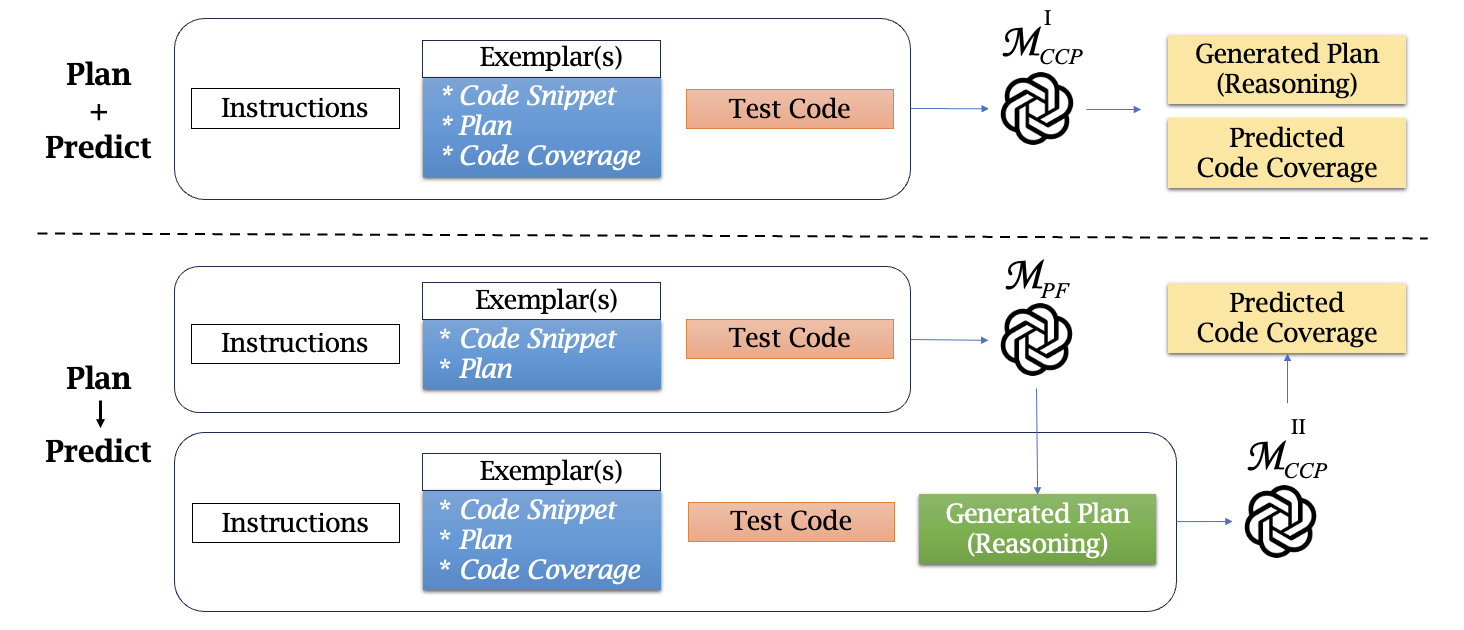
\includegraphics[width=0.7\linewidth]{codepilot-overview.png}
    \vspace{-19pt}
    \caption{Overview of {\cctool} Workflow for \textit{One-Prompt} (top) and \textit{Two-Prompt} (bottom) settings.}
    \label{fig:codepilot}
\end{figure}

Unlike in one-prompt {\cctool}, in this approach, we divide both \textit{Plan Formulation} and \textit{Code Coverage Prediction} in two prompts. The goal of the initial \textit{Plan Formulation} phase is to guide the LLM to \underline{\textit{reason}} about the given code snippet and construct a plan by itself, that is integral for navigating the code snippet and attaining an understanding of the execution flow. For this purpose, we leverage an LLM $\mathcal{M}_{PF}$ that takes as an input prompt: (a) a set of instructions $\mathcal{I}_{PF}$ describing the task; (b) an exemplar comprising a code snippet $\mathcal{C}$ (different from $\mathcal{C}_T$) and its corresponding plan $\mathcal{P}$; (c) the given code snippet $\mathcal{C}_T$. 
Here, $\mathcal{M}_{PF}$ utilizes the exemplar to guide the LLM to generate a similar plan $\mathcal{P}_T$ for $\mathcal{C}_T$.
%Let the LLM-generated plan for $\mathcal{C}_T$ be $\mathcal{P}_T$. 
This can be formulated as:
\begin{equation}\label{form:f1}
\textcolor{dkgreen}{\mathcal{P}_T} = \mathcal{M}_{PF} \textbf{\ \{\ } \mathcal{I}_{PF}, \langle \mathcal{C}, \mathcal{P} \rangle, \mathcal{C}_T \textbf{\ \}\ }  
\end{equation}

In \textit{Code Coverage Prediction} phase, the goal is to \underline{\textit{act}} on the code snippet $\mathcal{C}_T$ as per the LLM-generated plan $\mathcal{P}_T$ to enhance its execution-flow understanding, and predict the code coverage accordingly. For this purpose, we leverage an LLM $\mathcal{M}_{CCP}^{II}$ that takes as an input prompt: (a) a set of instructions $\mathcal{I}_{CCP}$ describing the task; (b) an exemplar comprising code snippet $\mathcal{C}$ and its plan $\mathcal{P}$ (same as in the \textit{Plan Formulation} phase), as well as its code coverage $\mathit{Cov}$; (c) the test code snippet $\mathcal{C}_T$; and (d) the LLM-generated plan $\mathcal{P}_T$.
Here, $\mathcal{M}_{CCP}^{II}$ utilizes the exemplar to guide the LLM to learn to determine the code coverage for the code example based on the program semantics-guided code execution plan. Subsequently, based on the $\mathcal{M}_{PF}$-generated plan $\mathcal{P}_T$ for the test code snippet, it predicts the code coverage $\mathit{Cov}_T$. 
This can be formulated as:
\begin{equation}
\textcolor{blue}{\mathit{Cov}_{T}} = \mathcal{M}_{CCP}^{II} \textbf{\ \{\ } \mathcal{I}_{CCP}, \langle \mathcal{C}, \mathcal{P}, \mathit{Cov} \rangle, \mathcal{C}_T, \textcolor{dkgreen}{\mathcal{P}_T} \textbf{\ \}\ }  
\end{equation}

\subsection{CFG-based Planning for Code Coverage Prediction}

%\subsection{Key ideas}

We aim to introduce a novel planning framework for code
execution, named \underline{O}bservation, \underline{R}easoning, and
\underline{C}ode-Driven, \underline{A}ction ({\orca}). {\orca} prompts
the GPT~\cite{chatGPT} to autonomously devising a plan for
predictive execution by traversing the CFG and
subsequently detecting the runtime errors.

\subsubsection{Teaching the LLM to `execute' the CFG}

%Guiding a model to navigate and predict the execution within a CFG
%offers advantages in mitigating the limitations of the aforementioned
%rudimentary approach, which dissects loop execution into
%fragments. Initially, despite segmenting execution into blocks,
%continuity of variable values from one block to the next can be
%preserved. This is reinforced by employing a "symbol table" to monitor
%relevant variable values within the current loop context. Secondly,
%traversing a cycle within the CFG mirrors iteration through the
%corresponding loop in the source code, while branching conditions in
%the CFG signify loop entry and exit criteria. Thirdly, edges
%connecting the blocks inherently depict control flows dictated by
%flow-altering statements. For instance, the \code{continue} statement
%at line 6 of Fig.~\ref{fig:motiv} is depicted by the edge labeled with '*' in Fig.~\ref{fig:cfg}.

Guiding a model to traverse and predict the execution in a CFG
provides benefits to address the issues with the above naive solution,
which `executes' a loop by breaking it up into fragments. First,
despite breaking the `execution' into CFG blocks, the propagation of the
values in the context of the previous block can be maintained. To
reinforce this, we leverage the usage of a {\em symbol table} that
tracks the variable values relevant to the current block. Second, the
traversal through a circle in the CFG corresponds to the iterating
through the corresponding loop in the source code, and the branching
condition in the CFG represents the loop-entering and loop-exiting
conditions. Third, the edges among the blocks automatically represent
the control flows that are decided by the flow-altering
statements, e.g., \code{continue}, etc.

%For example, the \code{continue} statement at line 6 of
%Fig.~\ref{fig:motiv} is represented by the edge marked by `*' in
%Fig.~\ref{fig:cfg}.


\subsubsection{Leveraging LLM-based Planning on CFG}

%Automated planning capability of a LLM is the ability to develop an
%efficient and effective process to generate plans or sequences of
%actions to break down a complex task to achieve a goal into smaller
%and manageable
%steps~\cite{valmeekam2023on,pallagani2023understanding}. Researchers
%have proposed different planning frameworks for LLMs to effectively
%tackle a range of tasks in several domains~\cite{tien}.

The automated planning capacity of an LLM refers to its adeptness in
devising a streamlined and productive method for crafting plans or
sequences of actions. These plans are designed to deconstruct a
complex task, enabling the achievement of a goal through a series of
smaller, manageable
steps~\cite{valmeekam2023on,pallagani2023understanding}. Researchers
have introduced diverse planning frameworks tailored for LLMs,
facilitating their effective handling of a multitude of tasks in
various
domains~\cite{zhuang2024toolchain,hu2023avis,yao2023react,prasad2023adapt}.
%
%In the planning techniques, reasoning traces assist the LLMs in
%deducing, monitoring, and refining action plans, while actions
%facilitate interaction with external sources, such as
%environments~\cite{prasad2023adapt,yao2023react}.
The planning techniques have demonstrated efficacy in mitigating
issues like hallucination and error propagation in LLMs when tackling
complex tasks~\cite{yao2023react}.

%We aim to leverage LLM planning to guide it to devise a plan that
%`executes' the code by walking through the CFG and dynamically decides
%the paths through the conditions. Specifically, we adapted
%ReAct~\cite{yao2023react} to our problem. ReAct~\cite{yao2023react} is
%a novel prompting-based planning paradigm to ``generate both reasoning
%traces and task-specific actions in an interleaved manner, allowing
%for greater synergy between the two: reasoning traces help the model
%induce, track, and update action plans, while actions allow it to
%interface with and gather additional information from external sources
%such as environments''~\cite{yao2023react}. ReAct was shown to
%overcome the issues of hallucination and error propagation in LLM in
%dealing with complext tasks. The three core conceptual elements in a
%ReAct plan work in an interleaving manner: 1) {\em observations}: the
%observations that the LLM makes regarding the current state of the
%system and task, 2) {\em reasoning}: the thoughts on reasoning to make
%the next move forward in the next step of the plan, and 3) {\em
%  actions}: the list of actions to be taken according to the reasoning
%in the next step. For example, in applying ReAct in robotics, one
%would write prompts according to the ReAct paradigm to instruct the
%LLM to develop a plan for a robot to observe the environment, make
%reasoning from external sources, and perform the actions accordingly.


\begin{wrapfigure}{r}{0.55\textwidth}
  \centering
  \footnotesize
	\lstset{
		numbers=left,
		numberstyle= \tiny,
		keywordstyle= \color{blue!70},
		commentstyle= \color{red!50!green!50!blue!50},
		frame=shadowbox,
		rulesepcolor= \color{red!20!green!20!blue!20} ,
		xleftmargin=1.5em,xrightmargin=0em, aboveskip=1em,
		framexleftmargin=1.5em,
                numbersep= 5pt,
		language=Python,
    basicstyle=\scriptsize\ttfamily,
    numberstyle=\scriptsize\ttfamily,
    emphstyle=\bfseries,
                moredelim=**[is][\color{red}]{@}{@},
		escapeinside= {(*@}{@*)}
	}
\begin{lstlisting}[]
@Initial Symbol Table:@
{n: (4, 'int'), total: (4, 'int'), i: (0, 'int')}

@Block 1:@
Statements: range(n)
- Execute range(n): [0, 1, 2, 3]

Condition: True (Always True for range(n))
- Go to Block 2

Updated Symbol Table:
{n: (4, 'int'), total: (4, 'int'), i: (0, 'int')}

@Block 2:@
Statements: i <- iterator
- Execute i <- iterator: i = 0

Condition: True (Always True iterator)
- Go to Block 3

Updated Symbol Table:
{n: (4, 'int'), total: (4, 'int'), i: (0, 'int')}

@Block 3:@
Statements: total += i, (i + total) % 2 == 0
- Execute total += i: total = 4 + 0 = 4
- Evaluate condition: (0 + 4) % 2 == 0 => 0 == 0

Condition: True
- Go to Block 4

Updated Symbol Table:
{n: (4, 'int'), total: (4, 'int'), i: (0, 'int')}
... 
...
total = 1 / (total - 13) = 1 / (13 - 13)) = 1 / 0
@The program crashes due to a divided by zero.@
\end{lstlisting}
\vspace{-6pt}
\caption{Example on LLM Planning}
\label{fig:motiv-gpt}
\end{wrapfigure}

Our objective is to harness planning to guide an LLM in formulating
its own plan for ``executing'' code by traversing the CFG and detect
the runtime errors/exceptions in the process. Inspired by
ReAct~\cite{yao2023react} planning technique, we aim to leverage three
conceptual elements in modeling a plan, which operates in an
interleaved manner: 1) {\em Observations}: These encompass the LLM's
observations regarding the current state of the system and task. 2)
{\em Reasoning}: This entails the cognitive processes involved in
determining the next step within the plan. 3) {\em Actions}:
These denote the sequence of actions to be undertaken based on the
reasoning next.

Within the context of our problem in runtime error detection,
{\em ``actions''} ($\mathcal{A}$) entail predictive execution, involving the
prediction of statement execution within a block, and updating the
symbol table to reflect variable values. {\em ``Observations''}
($\mathcal{O}$) involve retrieving variable values from the symbol
table. {\em ``Reasoning'' } ($\mathcal{R}$) encompasses evaluating conditions
at the conclusion of a block and, based on observations from the
symbol table, determining the subsequent actions for the next
block. This involves updating the symbol table and proceeding to
predictively execute statements in the next block. We introduce the
concept of a {\em Pause} for the LLM in reasoning during the CFG
traversal at the condition of a block. This makes the LLM focus on the
observations of the variables' values in the symbol table. We expect
this to help minimize the error propagation in value computation in
the LLM.

%introduce {\orca}, a novel planning framework for LLMs that is
%%%%%%=======> customized for predictive execution.
%Specifically, we have adapted ReAct~\cite{yao2023react} to address our
%problem domain. ReAct~\cite{yao2023react} introduces a novel
%prompting-based planning paradigm that enables the generation of both
%reasoning traces and task-specific actions in an interleaved
%manner. This approach fosters greater synergy between reasoning and
%action generation: reasoning traces assist the model in deducing,
%monitoring, and refining action plans, while actions facilitate
%interaction with external sources, such as
%environments~\cite{yao2023react}. ReAct has demonstrated efficacy in
%mitigating issues like hallucination and error propagation in LLMs
%when tackling complex tasks~\cite{yao2023react}.
%

%The ReAct planning framework revolves around three core conceptual
%elements, which operate in an interleaved manner: 1) {\em
%  Observations}: These encompass the LLM's observations regarding the
%current state of the system and task. 2) {\em Reasoning}: This entails
%the cognitive processes involved in determining the next step forward
%within the plan. 3) {\em Actions}: These denote the sequence of
%actions to be undertaken based on the reasoning in the subsequent
%step.

%In our research, we adapt ReAct to guide the LLM in formulating a plan
%for traversing the CFG and predicting outcomes. Within this framework,
%``actions'' entail predictive execution, involving the prediction of
%statement execution within a block, and updating the symbol table to
%reflect variable values. ``Observations'' involve retrieving variable
%values from the symbol table. ``Reasoning'' encompasses evaluating
%conditions at the conclusion of a block and, based on observations
%from the symbol table, determining the subsequent actions for the next
%block. This involves updating the symbol table and proceeding to
%predictively execute statements in the next block.



%In our work, we adapt ReAct to instruct the LLM to build a plan to
%traverse the CFG and predict the results. The {\em actions} refer to
%the {\em predictive execution} (i.e., the prediction of the execution)
%of the statements in a block and the {\em update the symbol table}
%regarding the variable values. The {\em observations} refer to the
%retrieval of the variable values in the symbol table. The {\em
%  reasoning} refers to the checking of the condition at the end of a
%block and based on the observations regarding the symbol table, making
%the decision on the actions to be taken for the next block (i.e.,
%updating the symbol table and proceeding to predictively execute the
%statements in the next block).

%Compare with ReAct: For instance, when applying ReAct in a robotics
%context, prompts are formulated following the ReAct paradigm to
%instruct the LLM in devising a plan for observing the environment,
%engaging with external information sources through reasoning, and
%executing actions accordingly.



Fig.~\ref{fig:motiv-gpt} partially shows the output plan and
prediction of GPT after our planning prompt (will be explained
later).
%With our prompt, GPT produces the plan and prediction as follows.
As seen, it first takes the observation on the initial symbol
table. Then, it starts predictive execution for Block 1, which
contains the computation of \code{range(n)}.  The reasoning at this
branching condition is that it is always \code{true}, leading to the
action of {\em `Go to Block 2'} and updating the symbol table.~The
interleaving process of observations, reasoning, and actions
continue for Block 2. The action in Block 2 includes only the
initialization of the iterator $i$.  The condition is \code{true}
leading to Block 3.  The series of actions in Block 3 begin with the
predictive execution of the statement \code{total += i}. At the
branching condition, the LLM follows its plan and stops to evaluate it
to \code{true}, leading to the reasoning of going to Block 4 and
updating the symbol table.  The process continues until
\code{$<$end$>$} is encountered.  As seen, the LLM was able to
autonomously develop a plan to predict the execution of the loop with
four iterations.

Another pivotal aspect for predictive code
execution is its departure from instructing the LLM
to halt the process after each cycle of observation, reasoning, and
action, as seen in ReAct~\cite{yao2023react}. This would~lead
to an excessive number of API calls to prompt the LLM (a call for each
block). For instance, in the scenario described, the process would
pause at each block, prompting the LLM to retrieve variable values
from the symbol table, which would then be written to a
file. Subsequently, a new prompt would be requested for the LLM to
begin a new cycle of observation (reading from that file),
reasoning, and action for the next block. Instead, {\orca}
simply instructs the LLM to pause at the condition of a block to
reduce error propagation. This streamlined approach also allows
{\orca} to make only one API call to prompt the LLM. {\orca} lets the LLM autonomously operate the cycle of operations,
reasoning, and actions without interruption. Note that
ReAct~\cite{yao2023react}, as being applied to robotics, needs
to instruct the LLM to stop after each cycle to observe the external
environment. {\orca} instructs the LLM to manage the symbol table,
instead of writing it to a file.

%Another key aspect of {\orca} framwork for predictive code execution
%is that it does not instruct the LLM to halt the process following
%each cycle of observations, reasoning, and actions as in
%ReAct~\cite{yao2023react}, which would result in too many API calls
%for prompting to the LLM (a call for a block). For example, in the
%above code, the process will stop at each block and the LLM would
%retrieve the variables' values from the symbol table, which would be
%written to a file. A new prompt is requested to the LLM for a new
%cycle of observation, reasoning, and actions for a new block.
%Instead, {\orca} simply tells the LLM to pause at the condition of a
%block to reduce error propagation. This also allows {\orca} to have
%only one API call for prompting to the LLM.

%\begin{figure}[t]



\section{Thrust 2. LLM-based Intelligent Test Case Generation}

%------------------- TEST CASE GENERATION PROMPTS FIGURE --------------------



%\subsection{The Test Case Generation Module}

\begin{wrapfigure}{l}{0.53\textwidth}
  \centering
	\lstset{
		numbers=left,
		numberstyle= \tiny,
		keywordstyle= \color{blue!70},
		commentstyle= \color{red!50!green!50!blue!50},
		frame=shadowbox,
		rulesepcolor= \color{red!20!green!20!blue!20} ,
		xleftmargin=1.5em,xrightmargin=0em, aboveskip=1em,
		framexleftmargin=1.5em,
                numbersep= 5pt,
		language=Java,
    basicstyle=\scriptsize\ttfamily,
    numberstyle=\scriptsize\ttfamily,
    emphstyle=\bfseries,
                moredelim=**[is][\color{red}]{@}{@},
		escapeinside= {(*@}{@*)}
	}
%\begin{minipage}{.48\textwidth}        
\begin{lstlisting}[caption = ]
(*@{\color{orange}{PROMPT} Coverage Increasing Test Case Generation@*)
Generate a single test case for a Java program to cover uncovered lines of code denoted by '!'. Provide only the test input without explanations. Consider various conditions, edge cases, and typical use cases.
The test case input is in the following:
Test Case Input:
<input 1>
<input 2>...
\end{lstlisting}
%\end{minipage}
\vspace{-6pt}
\caption{Prompt to generate test cases intended to increase coverage}
\label{fig:cov-prompt}
\end{wrapfigure}


This section presents the design of the interactions via prompting
between the LLMs used for test case generation.
%These prompting steps correspond to the two API calls to the LLM at
%line 7 and line 9 of Listing~\ref{algo}, and the call to coverage
%prediction LLM in CodePilot~\cite{forge24} at line 10 if
%Listing~\ref{algo}.
The Test Case Generation module, operated by prompting GPT, is
responsible for creating test mutations based on the coverage achieved
by the current test suite. Within {\tool}, we utilize a parameter
denoted as $N$, representing the number of test mutations
%(lines 7 and 9, Listing~\ref{algo})
that will be generated alongside the test seed $T\_seed$. Within the
test case generation loop,
%(line 5, Listing~\ref{algo}),
we implement two distinct strategies, each corresponding to a
different prompt and purpose. One strategy is devised to generate test
cases targeting various vulnerable areas, while the other strategy
focuses on each area individually to identify runtime
errors/exceptions.

\subsubsection*{Prompting for Coverage Increasing Test Case Generation}

As {\tool} functions as a coverage-guided fuzzing framework, increasing coverage stands as a primary objective. Consequently, if the cumulative coverage of the existing test suite hasn't yet achieved 100\%, and the generated test cases did not contribute towards reaching higher cumulative coverage, the immediate focus shifts to increasing code coverage in the subsequent cycle. This prompt responsible for Test Case Generation is directed to create test cases likely to extend coverage by targeting the portions of code that remain uncovered. (prompt depicted in Fig.~\ref{fig:cov-prompt}).





\begin{wrapfigure}{l}{0.53\textwidth}
	\lstset{
		numbers=left,
		numberstyle= \tiny,
		keywordstyle= \color{blue!70},
		commentstyle= \color{red!50!green!50!blue!50},
		frame=shadowbox,
		rulesepcolor= \color{red!20!green!20!blue!20} ,
		xleftmargin=1.5em,xrightmargin=0em, aboveskip=1em,
		framexleftmargin=1.5em,
                numbersep= 5pt,
		language=Java,
    basicstyle=\scriptsize\ttfamily,
    numberstyle=\scriptsize\ttfamily,
    emphstyle=\bfseries,
                moredelim=**[is][\color{red}]{@}{@},
		escapeinside= {(*@}{@*)}
	}
\hspace{8pt}
%\begin{minipage}{.4\textwidth}        
\begin{lstlisting}[caption = ]
(*@{\color{orange}{PROMPT} Runtime-error-detection Test Case Generation@*)
Generate a single test case without providing an explanation for to raise the following scenarios in a Java program:

InputMismatchException: Provide an input value that whose data type is different than the one specified. 
ArithmeticException: Test cases that could raise arithmetic exceptions include division by zero, overflow, underflow, and attempts to perform invalid operations such as taking the square root of a negative number.
NullPointerException: Create a scenario where a variable is explicitly set to null before usage.
NumberFormatException: Input a value that cannot be parsed to the expected data type (e.g., a non-numeric string).
ArrayIndexOutOfBoundsException or IndexOutOfBoundsException: Design input values that lead to accessing array or list indices beyond their bounds.
(Other types of runtime errors and exceptions)
Ensure the test case input is in the following:
Test Case Input:
<input 1>
<input 2>...
Generate a single test case without providing an explanation for the below Java program:
\end{lstlisting}
%\end{minipage}
\vspace{-12pt}
\caption{Prompt to generate test cases intended to catch errors}
\label{fig:exception-prompt}
\end{wrapfigure}

The sole purpose of the prompt is to produce a test case that
comprehensively covers lines of code not previously traversed by test
cases in the current suite. In the prompt, the LLM receives the code
coverage information of the current test suite, denoted by `$>$' and
`!' for covered and uncovered lines, respectively. We
also instruct the LLM to produce the output in a specific format,
where different scenarios are considered, such as negative,
positive, zero inputs, and maximum values, thus reflecting a
diverse range of inputs.

\subsubsection*{Prompting for Runtime-Exception-Detection Test Case Generation}

Once the target of achieving 100\% coverage is met or a test case
effectively covers previously unexplored code segments, the focus
shifts towards uncovering potential runtime exceptions.
%
This strategy is designed to prompt the LLM towards generating test
cases aimed at capturing runtime errors and
exceptions. Fig.~\ref{fig:exception-prompt} illustrates the structures
and intricacies of our prompt for this strategy. The initial segment
is dedicated to predicting and providing insights into various
potential unhandled runtime exceptions. The objective is to generate
test cases to explore diverse facets of runtime exceptions
comprehensively. We also instruct the LLM to output in a specific
format. We expect that this strategy complements the
coverage-increasing test case generating prompt to efficiently produce
high-quality test cases, thus delivering a thorough assessment of the
target program.

\subsubsection*{Preliminary Experimental Results on Runtime Error Detection}
\label{sec:rq1}

%\subsection{Baseline and Procedure}

{\bf Baselines and Metrics.} In this study, we chose Jazzer~\cite{jazzer}, an
open-source fuzz testing tool for Java due to its popularity and
availability.
%
Both coverage-guided fuzzing approaches were configured to operate
continuously for a duration of 5 minutes. For Jazzer, this limit
period encompasses the fuzzing process, which involves test case
generation, execution for coverage and bug detection, and the
integration of pertinent test mutations into the corpus for subsequent
testing iterations. Notably, the timeout duration excludes the build
and compilation phases to ensure fair comparison.  Conversely, for
{\tool}, the 5-minute limit encompasses all the steps within the
framework, that are
integral to its coverage-guided fuzzing workflow. Upon
reaching the time limit, the execution logs of both fuzzers are
scrutinized to gather metrics essential for evaluating their
respective performances.

%\subsection{Evaluation Metrics}

\begin{wrapfigure}{l}{0.53\textwidth}
\begin{center}
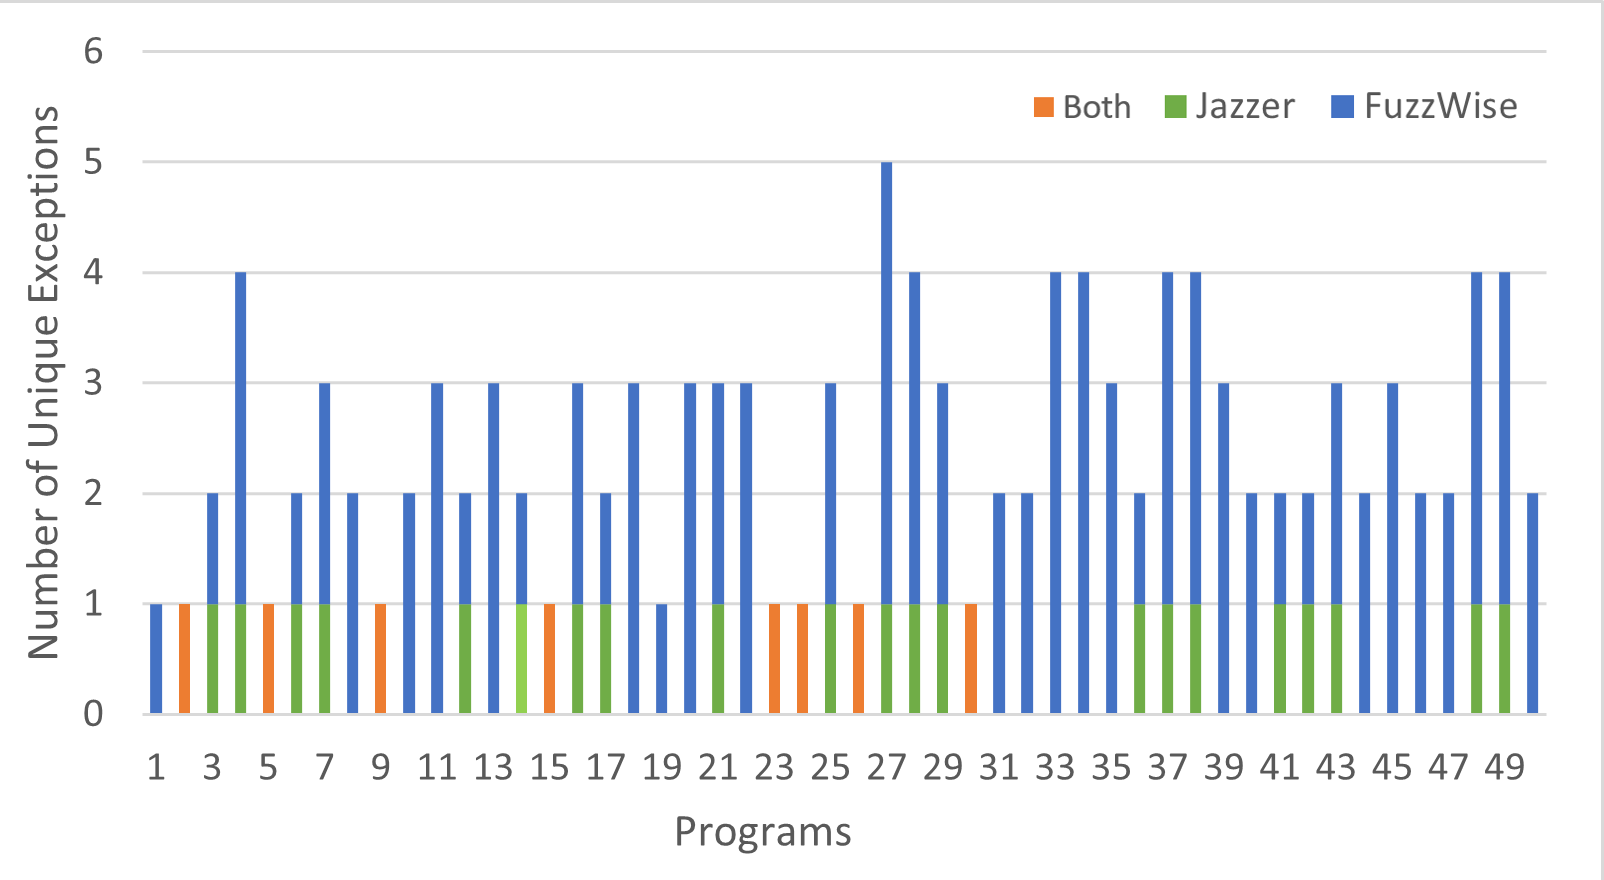
\includegraphics[width=3.5in]{RQ1a_Unique Exceptions.png}
\vspace{-21pt}
\caption{Comparative Study on Runtime Error Detection}
\label{fig:rq1-runtime-detection}
\end{center}
\end{wrapfigure}

First, we aim to measure the approaches' effectiveness in detecting
runtime errors. Within the time limit, we counted the number of unique
runtime errors/exceptions that an approach can reveal for a
program.

%This is denoted by the Number of Unique Runtime Exceptions (\code{NURE}).

Second, we also aim to measure how the test generation processes from
the approaches perform in terms of the~numbers of test cases created,
wasted, executed, and the number of effective test
cases. Thus, we use the following metrics for this study: Average
Generated Test cases (AGT), Average Executed Test cases (AXT), Average
Effective Test cases (AET), and Average Wasted Test cases (AWT). AGT
is computed as the average number of generated test cases for each
approach. AXT denotes the average number of test cases that were
actually executed on the programs to detect runtime exceptions. AET
denotes the average number of test cases that effectively detected
runtime errors. AWT signifies the average number of test cases
wasted due to their lack of influence on either coverage
improvement or bug detection. We also stratify these metrics over the
different ranges of the programs' lengths.

%It is determined as the ratio of the total number of discarded test cases by the fuzzer for all programs within a particular code length range to the number of programs within that range.

%It is computed as the ratio of the total number of executed test cases for all programs within a specified code length range to the number of programs in that range.



%In order to correctly evaluate the performance of {\tool} against Jazzer as a baseline, there are 2 crucial elements that must be compared i.e.,  the number of exceptions raised within a specified time frame, and the number of test case mutations that are not of significance to the fuzzer and are therefore, discarded. 

%To assess the performance of Jazzer and {\tool} across the dataset, we employ two types of metrics. The first type aims to evaluate performance based on the number of test cases created, executed, and discarded. Two metrics are utilized for this purpose: Average Executed Test cases (AET), and Average Discarded Test Cases (ADT).



%In summary, AET and ADT metrics provide insights into the behavior of the fuzzer concerning the execution, and discarding of test cases for programs of specific lengths. These metrics offer approximate values indicating the expected number of test cases executed, and discarded, respectively, for a given program length.

%The second type of metrics focuses on evaluating the performance of the coverage-guided fuzzers based on the number of runtime exceptions they can raise within a specified time limit. This is measured by a singular metric known as the Number of Unique Runtime Exceptions (NURE), which quantifies the unique runtime exceptions caught by the fuzzer for a single program.

%\subsection{Empirical Results}



% Figure 8 accurately depicts the NURE (Number of Unique Runtime Exceptions) values for each of 50 programs in the dataset. The maximum NURE value acheived by Jazzer (depicted im green) is 1 Exception per program wheres the maximum acheived by {\tool} is 5 exceptions in a program. It is evident that {\tool} is able to detect equal to more number of unique runtime exceptions than Jazzer for the same program within the same time frame due to the fact that {\tool} dual prompting method for test case generations.

% Additionally, When considering the number of Test Cases generated (refer to Figure 6), {\tool} generates close to 0.0065\% of the number of test cases that Jazzer generates for a program and still is successful in raising more number of unique runtime exceptions. This can be attributed to the fact that the test case mutations generated by {\tool} are more controlled and less random than Jazzer. 

% When it comes to test case execution, Jazzer executed all of the test cases that it generates, irrespective of the presence of duplicate test cases. On the other hand, {\tool} executes an average of 235 out of 315 test cases generated. This is because, before execution, {\tool} removes duplicate test cases to increase efficiency. 

% Finally, when comparing the number of test cases that both fuzzers discard due to ineffectivness or duplicacy (refer to figure 7), across a range of code length, Jazzer discards an average of 4679532 test cases for a code of length 10 to 15 lines whereas {\tool} discards an average of 305 test cases. For code of length 16-20 lines, Jazzer discards 2389922 of the test cases it generates whereas {\tool} only discards 73 of the generated test cases. For code of length  21 to 40 lines, Jazzer discards 3374709 of the test cases it generates and executes whereas {\tool} discards 23. For code length of 41 to 60 lines and 61 to 70 lines, Jazzer discards XXX(NEED TO VERIFY) and 1624254 test cases respectively whereas {\tool} discards none of the test cases it generates. {\tool} extremely low percentage of the number of test cases discarded can be attributed to the higher quality of the test case mutations generated. Since very less mutations are generated more than once, fewer have to be discarded. 

% It is also impoartant to note that as the average length of code increases, AGT, AET and AGT for both fuzzers consistently drops due to the fact that the time taken to both execute and predict the code coverage for a single test case increases with an increase in length of code.

%Fig.~\ref{fig:rq1-runtime-detection} displays the runtime error
%detection results. As seen, {\tool} is able to detect more runtime
%errors/exceptions than the baseline Jazzer. Within the time limit,
%while Jazzer can only detect at most one runtime error, {\tool} can
%detect up to 5 runtime errors. In {\bf XX} cases, Jazzer is not
%effective, while {\tool} did not detect any exception in only two
%programs.  In all 50 programs, within the time limit, {\tool} detected
%a total of {\bf XX} runtime errors, while {\tool} revealed a total of
%{\bf YY} such errors.
 
%accurately illustrates the NURE (Number of Unique Runtime Exceptions) values for each of the 50 programs within the dataset. Jazzer achieved a maximum NURE value of 1 exception per program (depicted in green), whereas {\tool} reached a maximum of 5 exceptions in a program. This indicates that {\tool} is capable of detecting a greater number of unique runtime exceptions than Jazzer for the same program within the same time frame, owing to {\tool}'s dual prompting method for test case generation.



{\bf Preliminary Results.} Fig.~\ref{fig:rq1-runtime-detection}
presents the results on runtime error detection. As seen, {\tool}
outperforms the baseline Jazzer in detecting more unique runtime
errors/exceptions. While Jazzer, within the time limit, can only
detect a maximum of one runtime error, {\tool} can identify up to 5
runtime errors. In {\bf 17} cases, Jazzer proves ineffective (no
detected error), whereas {\tool} only failed to detect any exceptions
in {\bf 3} programs. Across all 50 programs, within the given time
constraints, {\tool} successfully identified a total of {\bf 97}
runtime errors, while Jazzer only detected {\bf 26} such errors.



% \begin{figure}[t]
% \begin{center}
% \includegraphics[width=4.5in]{rq1_table.png}
% \vspace{-15pt}
% \caption{Comparison on Test Case Generation (RQ1) ({\bf FIXME} Remove ADT, add Effective Test Cases (AET), change the old AET into AXT)}
% \label{fig:rq1-agt-aet-adt-table}
% \end{center}
% \end{figure}

\begin{wraptable}{l}{0.62\textwidth}
  \centering
  \small
  \caption{Comparison on Test Case Generation}
\label{tab:rq1coverageeval}
%\renewcommand{\arraystretch}{1.2} % Adjust the vertical spacing
%\resizebox{\columnwidth}{!}{%
\begin{tabular}{c|ccc|ccc}
\hline
\multirow{2}{*}{\textbf{Length of Code (Lines)}} & \multicolumn{3}{c|}{\textbf{Jazzer}} & \multicolumn{3}{c}{\textbf{FuzzWise}} \\ \cline{2-7} 
 & \multicolumn{1}{c|}{AGT} & \multicolumn{1}{c|}{AXT} & AET & \multicolumn{1}{c|}{AGT} & \multicolumn{1}{c|}{AXT} & AET \\ \hline
10 to 15 & \multicolumn{1}{c|}{8,083,663} & \multicolumn{1}{c|}{8,083,663} & 4,009,232 & \multicolumn{1}{c|}{513} & \multicolumn{1}{c|}{251} & 181 \\
16 to 20 & \multicolumn{1}{c|}{5,040,462} & \multicolumn{1}{c|}{5,040,462} & 2,520,225 & \multicolumn{1}{c|}{249} & \multicolumn{1}{c|}{176} & 128 \\
21 to 40 & \multicolumn{1}{c|}{3,374,709} & \multicolumn{1}{c|}{3,374,709} & 1,147,240 & \multicolumn{1}{c|}{197} & \multicolumn{1}{c|}{174} & 122 \\ 
41 to 60 & \multicolumn{1}{c|}{2,918,978} & \multicolumn{1}{c|}{2,918,978} & {661,458} & \multicolumn{1}{c|}{118} & \multicolumn{1}{c|}{118} & 66 \\
61 to 70 & \multicolumn{1}{c|}{1,667,523} & \multicolumn{1}{c|}{1,667,523} & 372,470 & \multicolumn{1}{c|}{99} & \multicolumn{1}{c|}{99} & 65 \\ \hline
\end{tabular}%
%}
%\vspace{4pt}
\end{wraptable}

Table~\ref{tab:rq1coverageeval} shows the detailed results.
%on the number of generated test cases (\code{AGT}), the number of
%executed test cases (\code{AET}), and the number of discarded test
%cases (\code{ADT}).
We group them accordingly to the sizes of the programs. As seen,
regarding the number of generated test cases, {\tool} produced
significantly fewer test cases, accounting for approximately 0.0065\%
of the number of test cases generated by Jazzer for a given
program. However, despite this disparity, {\tool} successfully
identified more unique runtime exceptions.

Regarding the executed test cases, Jazzer, by design, executed all
generated test cases, including duplicates. In contrast, {\tool} {\em
  executed an average of 235 out of 315 generated test cases}. On
average, Jazzer executed {\bf 4,217,067} test cases per program, while
{\tool} executed only {\bf 235} test cases. Combined with the findings
depicted in Fig. \ref{fig:rq1-runtime-detection}, it's evident that
{\tool} is more efficient in runtime error detection compared to the
baseline: on average, {\tool} executed {\bf 1,742,125} generated test cases
to detect a runtime error, while Jazzer executed {\bf 112} test cases
per exception.

%{\bf Add a paragraph to discuss the result in the Fig. about the
%  generated test cases that are effective in bug detection. Also, add
%  the ratio between the number of effective test cases over the number
%  of generated test cases}.

%Regarding effective test cases, as seen in
%Fig.~\ref{fig:rq1-runtime-detection}, on average, {\tool} generates a
%higher number of effective test cases than Jazzer, i.e., more
%effective in error detection, {\bf XX} versus {\bf YY}. Additionally,
%the ratio between the number of effective test cases over the total
%number of generated ones for {\tool} ({\bf XX}) is also higher than that
%ratio for Jazzer ({\bf YY}). This shows that {\tool} is more efficient
%in effective test case generation.

In terms of effective test cases, as depicted in
Fig.~\ref{fig:rq1-runtime-detection}, {\tool} generates a higher
average number of effective test cases compared to Jazzer, indicating
greater effectiveness in error detection ({\bf 112} versus {\bf
  2,158,456}). Moreover, the ratio of effective test cases to the total
number of generated test cases for {\tool} ({\bf 47.65\%}) is higher than
that for Jazzer ({\bf 41.31\%}). This underscores the superior efficiency
of {\tool} in generating effective test cases.

\begin{wrapfigure}{l}{0.52\textwidth}
\begin{center}
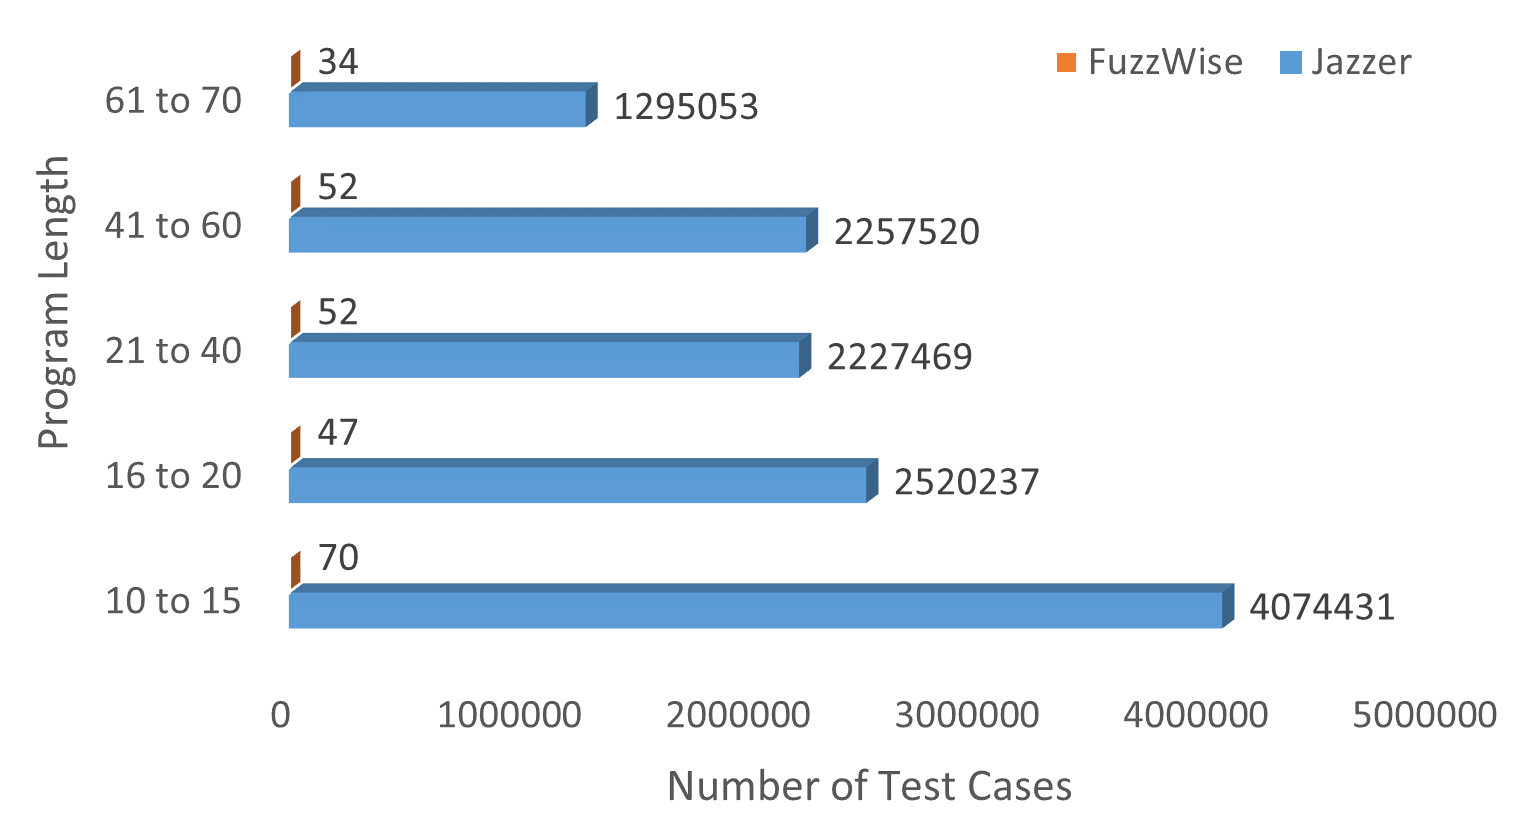
\includegraphics[width=3.5in]{RQ1b_Discarded Test Cases.png}
\vspace{-20pt}
\caption{Comparison on Test Case Execution and Dismissal}
\label{fig:rq1-agt-aet-adt-graph}
\end{center}
\end{wrapfigure}

Fig.~\ref{fig:rq1-agt-aet-adt-graph} provides a visual comparison
between {\tool} and Jazzer regarding the number of test cases that
were wasted. In the case of Jazzer, these include the test cases
generated through mutations and executed but did not detect any
runtime errors, nor were they included as test seeds for subsequent
test generation cycles. This corresponds to the wasted resources in
the execution of those wasted test cases.  For {\tool}, we counted
towards this metric the generated test cases that were not included in
the final test suite, as well as those that were executed but did not
reveal any runtime errors. As depicted in
Fig.~\ref{fig:rq1-agt-aet-adt-graph}, Jazzer wasted a significantly
higher number of test cases compared to {\tool} across various code
length ranges. For example, for code snippets with 10--15 lines,
Jazzer discards/wastes an average of 4,074,431 test cases, while
{\tool} discards only {\bf 305} test cases. This trend
continues as code length increases, with Jazzer consistently
discarding a substantial number of test cases, whereas {\tool}
discards fewer or none, indicating the higher quality of its test case
generation. This also implies that {\tool} saves a large amount of
execution resources.

It is evident that as all the metrics for both fuzzers consistently decrease (Table~\ref{tab:rq1coverageeval} and Fig.~\ref{fig:rq1-agt-aet-adt-graph}). This trend is attributed to the increased time required to execute and predict code coverage for longer code lengths.

%As seen, regarding the number of test cases generated, {\tool}
%generated a signficantly smaller number of test cases: approximately
%0.0065\% of the number of test cases generated by Jazzer for a
%program, yet it successfully detected a higher number of unique
%runtime exceptions. 

%Furthermore, in terms of the number of test cases generated (refer to Figure 6), {\tool} generated approximately 0.0065\% of the number of test cases generated by Jazzer for a program, yet it successfully raised a higher number of unique runtime exceptions. This can be attributed to the controlled and less random nature of the test case mutations generated by {\tool} compared to Jazzer.

%Regarding the generated test cases that were actually executed, due to
%its design, Jazzer executed all of the generated ones (including the
%duplicate ones), while {\tool} executed an average of 235 out of 315
%generated test cases. For each program, Jazzer on average executed
%{\bf XX} test cases, while {\tool} executed only {\bf XX} test cases.
%Coupled with Fig.\ref{fig:rq1-runtime-detection}, {\tool} is more
%efficiently in runtime error detection than the baseline. On average,
%{\tool} executed {\bf XX} generated test cases to detect a runtime
%error, while Jazzer executed {\bf XX} test cases for an exception.

%Tien: discarded test cases
%Fig.~\ref{fig:rq1-agt-aet-adt-graph} visually displays the comparison
%between {\tool} and Jazzer regarding the numbers of test cases that
%were `disregarded'. For Jazzer, those are the test cases that were
%generated through mutations and executed, but did not detect any
%runtime errors nor were put back as the test seeds for the next cycles
%of test generation.  For {\tool}, we counted toward it the generated
%test cases that were generated, but not included in the final test
%suite and the ones that were executed but did not reveal any runtime
%errors. As seen in Fig.~\ref{fig:rq1-agt-aet-adt-graph}, Jazzer
%discards a significantly higher number of test cases compared to
%{\tool} across various code length ranges. For instance, for code snippets
%with 10--15 lines, Jazzer discards an average of 4,679,532
%test cases, whereas {\tool} discards only 305 test cases. As code
%length increases, Jazzer continues to discard a substantial number of
%test cases, whereas {\tool} discards fewer or none, indicating the
%higher quality of its test case generation.

%From Table~\ref{fig:rq1-agt-aet-adt-table} and
%Fig.~\ref{fig:rq1-agt-aet-adt-graph}, it is noteworthy that as the
%average code length increases, the metrics AGT (Average Generated Test
%cases), AET (Average Executed Test cases), and AGT (Average Discarded
%Test Cases) for both fuzzers consistently decrease due to the
%increased time required to execute and predict code coverage for
%longer code lengths.

%Moreover, when comparing the number of discarded test cases due to ineffectiveness or duplication (refer to Figure 7), Jazzer discards a significantly higher number of test cases compared to {\tool} across various code length ranges. For instance, for code lengths of 10 to 15 lines, Jazzer discards an average of 4,679,532 test cases, whereas {\tool} discards only 305 test cases. As code length increases, Jazzer continues to discard a substantial number of test cases, whereas {\tool} discards fewer or none, indicating the higher quality of its test case mutations, as seen in Figure 6.

%Regarding test case execution, Jazzer executed all generated test cases regardless of duplicate instances, whereas {\tool} executed an average of 235 out of 315 test cases generated.

%This difference arises because {\tool} removes duplicate test cases before execution to enhance efficiency.

%Tien: talk about the ratio of executed test cases over the detected exceptions












%\section{Thrust 3. Neural Symbolic Execution Infrastructure}
\label{sec:thrust3}

\section{Thrust 3. LLM Multi-agents and Pre-trained Language Models for Predictive Execution}
\label{sec:thrust3}

\subsection{Key Ideas}

In this work, we advocate for an emerging execution paradigm that we
call {\bf predictive execution}, PredEx. In predictive execution,
similar to the traditional execution, a program is provided with
specific input value. However, the execution is not carried out with
the computer performing the instructions in the program. Instead, a
trained machine learning (ML) model predicts the execution step based
on the specific input value. As a result, the execution path
corresponding to the input is derived. Predictive execution offers
several benefits in different usage scenarios in software development.

First, predictive execution is particularly useful in the scenarios
that the actual execution requires a dedicated environment or
hardware, thus, becomes prohibitively challenging. 

Second, predictive execution can serve as a building block for the
execution of incomplete code snippets, which are rendered as
inexecutable. By predicting the execution steps of inexecutable code,
it becomes possible to detect potential bugs early on. This
application could be particularly useful for identifying problematic
code snippets in online forums like StackOverflow, where there may be
instances of vulnerable code that can be migrated to a
codebase~\cite{verdi-tse22}. Such early detection avoids wasting
effort from developers to integrate the inexecutable code snippets
from online forums into a project.

Third, in software testing, by predicting the execution path
corresponding to an input, we can estimate code coverage without
executing every test case in the test
suite~\cite{ball-toplas94,elbaum-icsm01}. This is crucial for
debugging in security contexts, where executing untrusted code could
lead to vulnerabilities or system compromises. Predictive execution
allows for the analysis of potentially harmful or untrusted
code. Thus, the potential risks associated with running unverified or
potentially malicious code are mitigated.

%In the context of fuzz testing~\cite{fuzzing-testing-survey-2020},
%where test cases are generated automatically to explore program
%faults, predictive execution can help determine if a newly generated
%test satisfies the conditions required by a fuzzing engine to exercise
%a particular path. This capability allows for a more targeted and
%efficient model to fuzzing, potentially leading better bug
%detection. Moreover, with the predicted code coverage, fault
%localization can be enabled for those cases.

%In pursuit of predictive execution, the state-of-the-art
%approaches~\cite{liu2023code,ding2023traced} aim to predict execution
%traces and associated variable values along the way. However, they
%exhibit certain key limitations. TRACED~\cite{ding2023traced} does not
%handle well the code featuring iterative structures, while
%CodeExecutor~\cite{liu2023code} does not perform well for the
%execution with runtime errors and control flow statements (such as
%\code{return}, \code{break}, \code{continue}). The precision in
%predicting execution traces remains modest. We observed that these
%approaches place a substantial burden on models to grasp the
%transformation patterns from the entire program and input values to
%the full execution traces.

We propose a novel approach called {\bf PredEx} for predictive execution, which predicts the execution trace of a Python program based on its input. We design a new technique called {\bf blended analysis}, combining the strengths of both {\em Static Program Analysis} (PA) and {\em Large Language Models} (LLMs) to predict the next executed statement and execution trace given a Python program and its input. While LLMs like GPT-3.5~\cite{GPT3.5}, CodeT5~\cite{wang2023codet5}, Code Llama~\cite{code_llama}, 
%RoBERTa{liu2019roberta},
and others have demonstrated proficiency in comprehending source code,
their direct application in predicting execution traces for an entire
program with its input is constrained by various dynamic intricacies
of code execution. Conversely, while static PA can have a
correct~solution in some task, it tends to overestimate the actual
paths taken during execution.

\subsection{Predictive Execution Algorithm via Blended Analysis between PA and ML}

\begin{wrapfigure}{r}{0.6\textwidth}
%\begin{figure*}[t]
\begin{center}
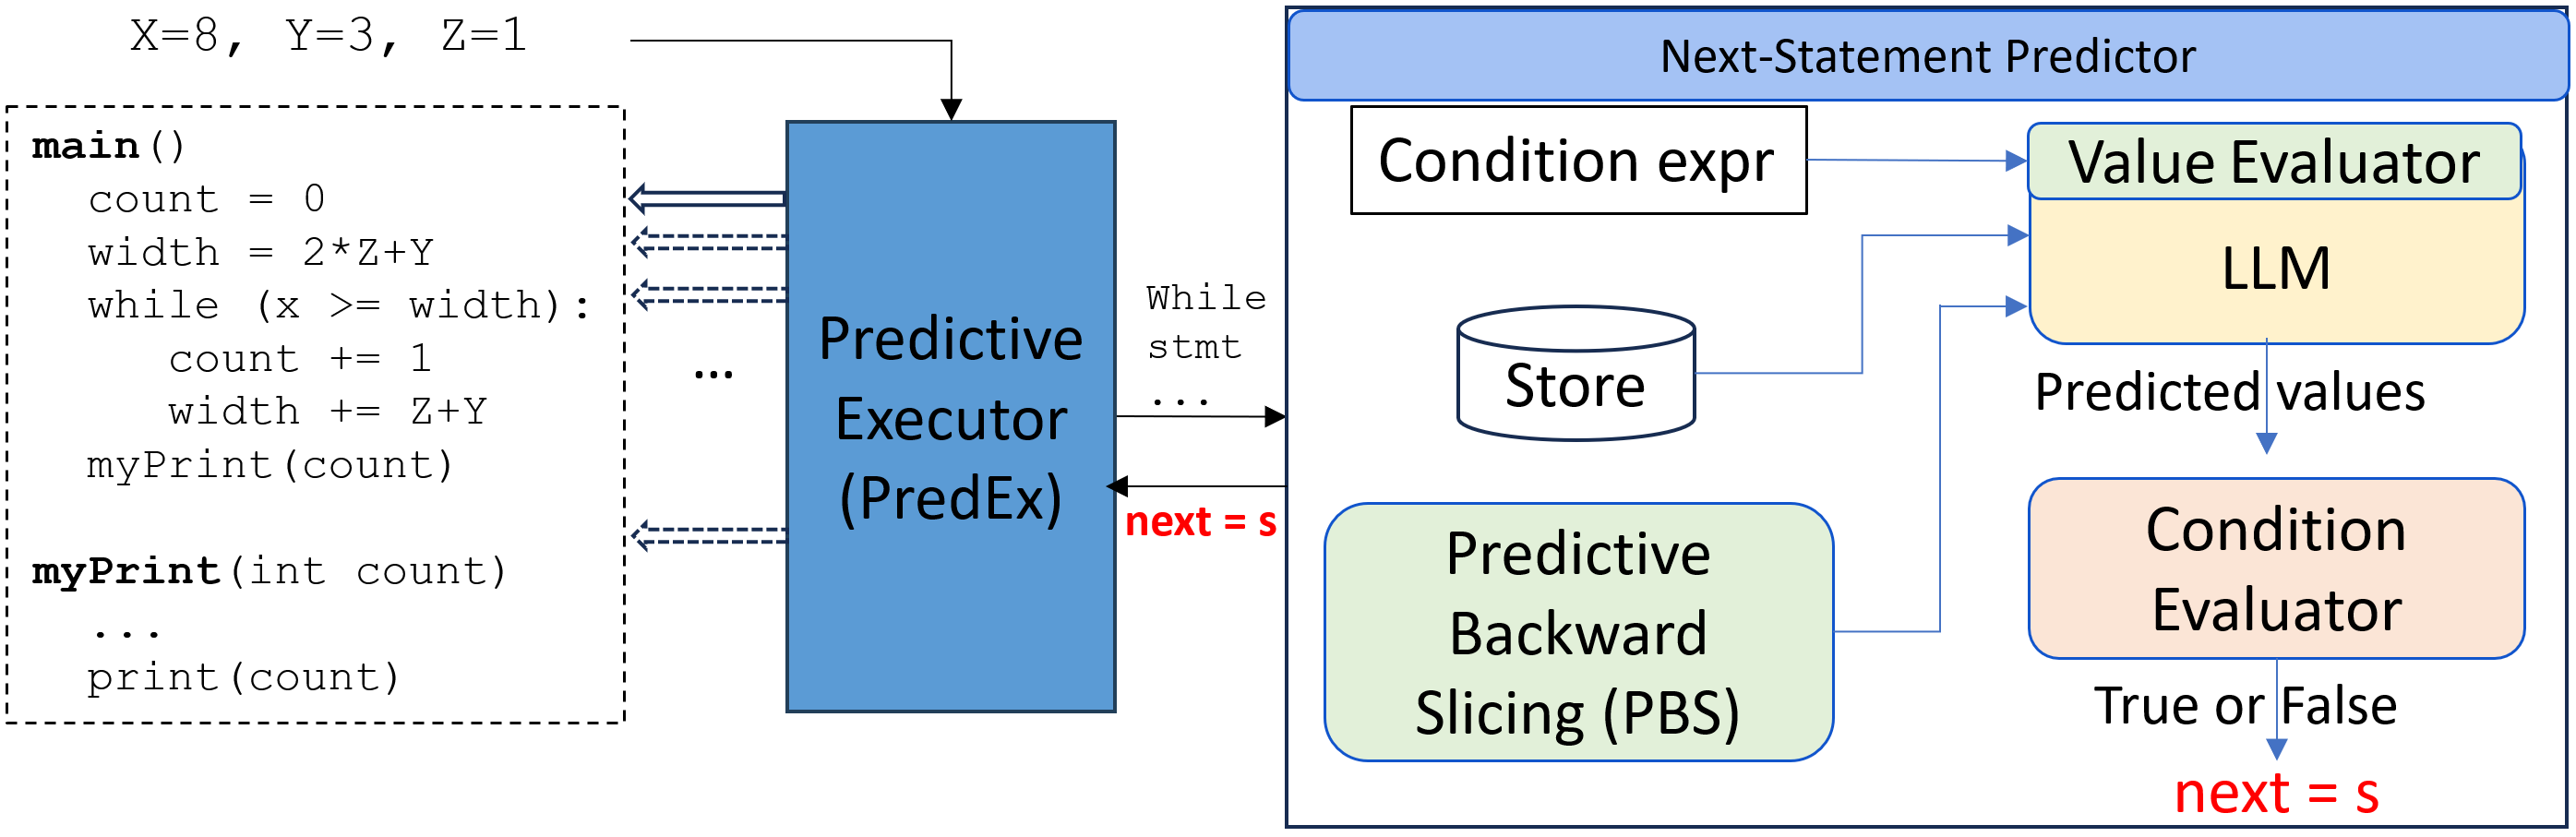
\includegraphics[width=4in]{overview-4.png}
\vspace{-22pt}
\caption{PredEx: Blended Analysis Framework for Predictive Execution}
\label{fig:overview}
\end{center}
%\end{figure*}
\end{wrapfigure}

In blended analysis, we decompose the original problem into smaller sub-tasks and allocate~each task to either PA or LLM based on their respective strengths. At the coarse-grained level, we divide the predictive execution problem into predicting the next executed statement at each step. When PA can make deterministic decisions, such as determining the next executed statement within a block, we leverage PA for that to alleviate the potential inaccuracy of the LLM. However, when PA is unable to ascertain the execution flow, particularly at branching points (e.g., \code{if}, \code{while}, \code{for}, etc.), we enlist the LLM to handle tasks critical for the decisions at those branching points. At the fine-grained level of the task of LLM-based branching decisions, we also harness PA to assist the LLM in focusing on the pertinent statements when making decisions about the branching direction. That is, we posit that by providing the LLM with support from PA and feeding it relevant statements, we can guide it in reasoning about the execution of a smaller subset of statements without executing them. Via pre-training, LLMs have learned patterns, logic, and reasoning capabilities that enable them to predict program execution for a smaller set of statements relevant to branching decisions.

%=====================================================
Specifically, the two sub-tasks at a branching point for the LLM
include {\em value evaluator} and {\em condition evaluator}. First, the value
evaluator focuses on determining the values of variables involved in
decision-making at a branching point. By using backward slicing
starting from those variables, we can help the LLM focus only on the
relevant, important statements that influence the values of the
variables. We build the backward slices and use the current predicted
statements and paths in the trace to approximate the dynamic backward
slice. Let us call it {\em predictive backward slice}. By such slices
and predicted values, we enable the LLM to recognize patterns and
dependencies in the code that affect the values of the current
variables. By training the LLM via few-shot learning on the external
API calls, we enable it to derive the output values of such calls.
Second, the condition evaluator, builds on the values obtained from
the value evaluator. Given the values of the variables at a branching
point, the condition evaluator can predict the outcome of the
condition expression. For this evaluation, one can have different
strategies. First, one can leverage the LLM as in the value
evaluator. Second, one can leverage the expression evaluator. Third,
one could build his/her own probabilistic condition evaluator to
estimate the probability of the condition being true.



%Fig.~\ref{fig:overview} shows an overview of PredEx. It accepts a
%Python program and input values. Its output is the predictive
%execution trace, i.e., the order of the statements that would be
%executed. The principle in PredEx is a {\bf blended analysis} between
%{\bf program analysis} and {\bf Large Language Model (LLM)}. The
%blended analysis is expressed in two folds. \underline{First}, when PredEx is
%certain on the execution order of the next statement $s$ based on the
%current statement, it will add $s$ into the resulting predictive
%execution trace. Only when it is not certain, e.g., at a branch of an
%\code{if} statement with an uncertain condition, PredEx requests its
%next-statement predictor (NSP) to provide the prediction of the
%potential next statement. \underline{Second}, even though we leverage LLM to
%predict the values of relevant variables and sub-expressions in the
%condition expression of a statement with a branching instruction, we use
%{\bf program analysis}, specifically the {\bf predictive backward slicing},
%to help the LLM pay attention only to the statements that might affect
%the evaluation of the condition. The backward slice for a variable
%might be long, thus, we design a strategy to optimize and shorten the
%slice by storing the predicted values of relevant variables at the
%latest prediction~point.

%With the blended analysis, we break down the task of predicting the
%execution into a smaller sub-tasks and leverage the deterministic
%nature of some sub-tasks (e.g., unconditional execution). We expect to
%help the LLM better decide the next executed statement.  In fact, in
%our empirical evaluation, PredEx improves over the state-of-the-art
%approaches, GPT-3.5~\cite{ChatGPT} and CodeExecutor~\cite{liu2023code},
%in which the source code and input are fed into the LLM to produce the
%entire execution trace.

\subsection{Predictive Execution: Illustrating Example}
\label{sec:example}

%\begin{figure}[htp]

\begin{wrapfigure}{r}{0.5\textwidth}
%\begin{figure}[t]  
\begin{center}
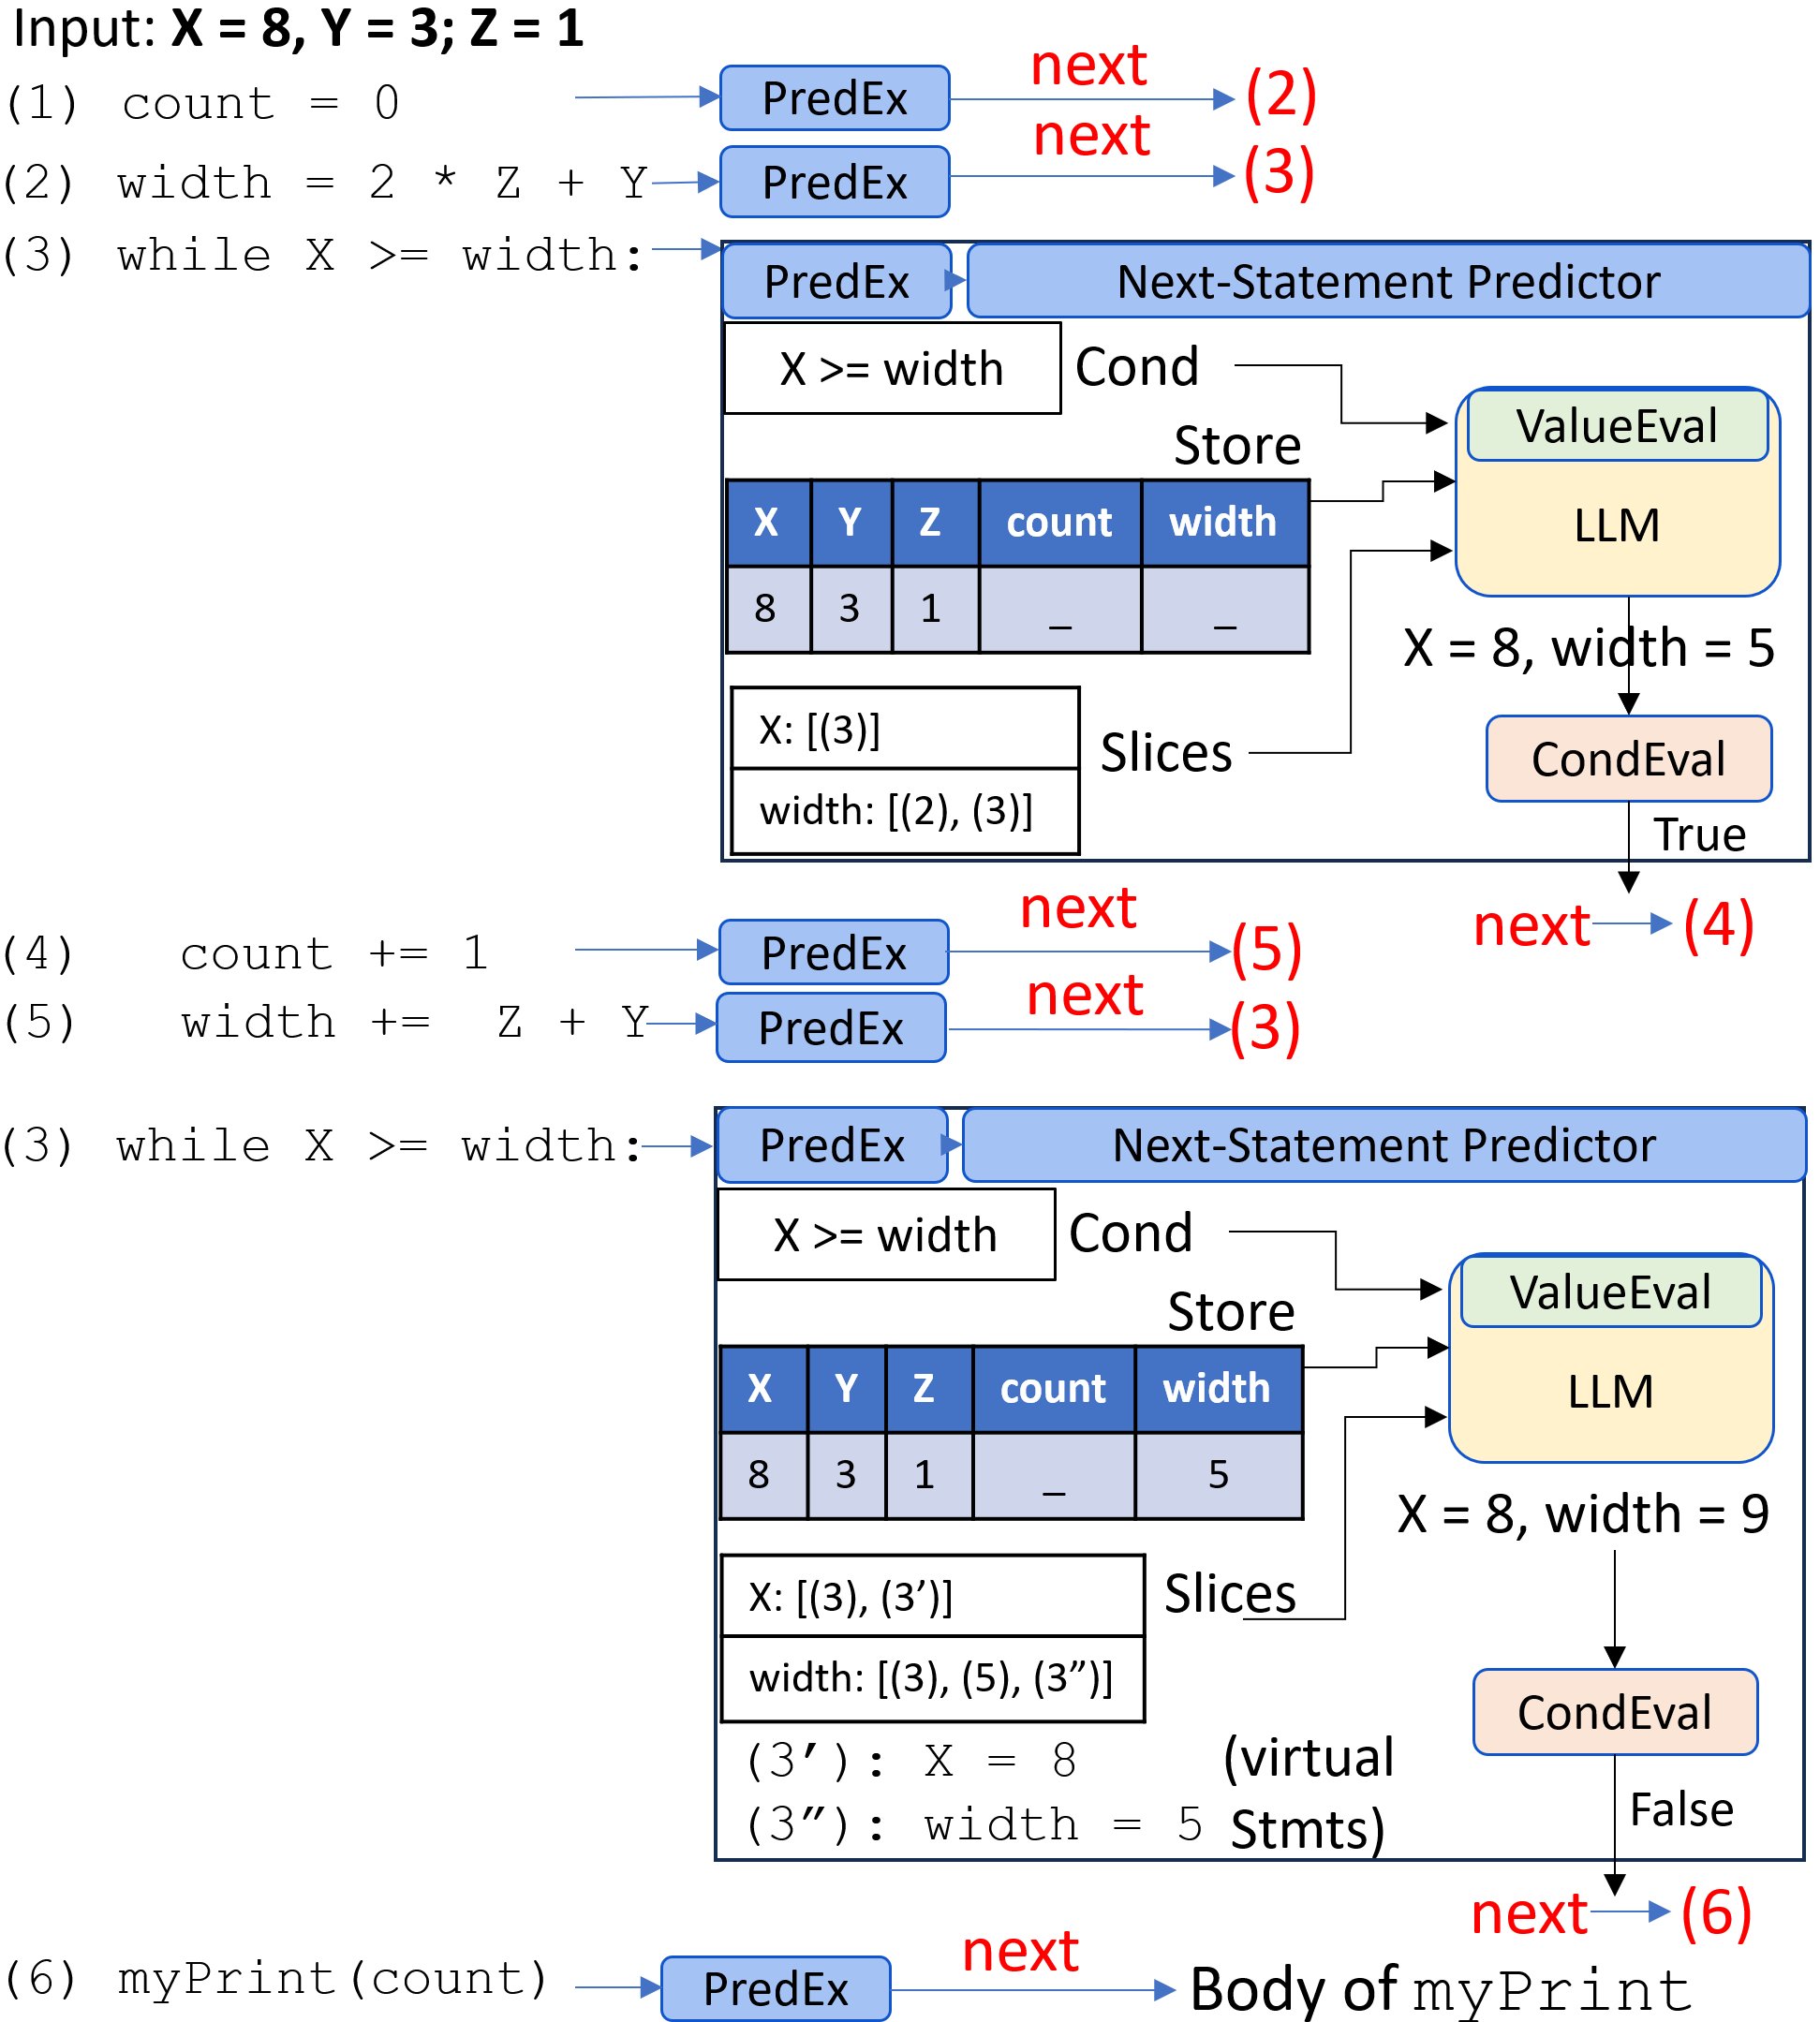
\includegraphics[width=3.2in]{example-4.png}
\vspace{-13pt}
\caption{Predictive Execution: An Illustrating Example}
\label{fig:illustration}
\end{center}
%\end{figure}
\end{wrapfigure}

Fig.~\ref{fig:illustration} illustrates how PredEx works on our
motivating example. For brevity in the figure, we use the new input
\code{X}=$8$, \code{Y}=$3$, and \code{Z}=$1$. Assume that, PredEx
starts with the assignment at line (1). Because line (1) is a simple
statement, PredEx decides the statement (2) to be the next
one. Similarly, PredEx decides the statement (3) as the one after
that.

At line 3, encountering a \code{while} statement, PredEx passes the
information on to the next-statement predictor. This LLM-based value
evaluator requires three pieces of information as
input. First, PredEx extracts the condition expression \code{X >=
  width}. Second, the current state of the value store $\theta$ includes the
initial values for the variables \code{X}=$8$, \code{Y}=$3$, and \code{Z}=$1$, and
the undefined values for \code{count} and \code{width} because those are the
values from the latest prediction point (also referred to as {\em
  check point}). If there is no prediction point yet, the latest check
point is at the very beginning. Third, PredEx computes two predictive
slices for the two variables involving in the condition
\code{X>=width}. The slice for \code{X} includes only the statement at line
(3), while the slice for \code{width} includes two statements at line (2)
and line (3).

From the three pieces of information, the LLM-based value evaluator
predicts the values of \code{X}=$8$ and \code{width}=$5$. After the store is
updated, the condition evaluator
will use it to evaluate \code{X>=width} and return $True$. To reduce
the number of requests to the LLM to update the values for all
variables, we only update the values of the variables involving in the
condition. For example, the value of the variable \code{count} is not
updated. The next prediction for the second iteration
will use the updated values in the store $\theta$. Because the
condition is predicted as $True$, the next-statement predictor will
return the statement (4) as the one.
%
Because the statement (4) is simple, PredEx decides the
statement (5) as the next one. Similarly, it moves on to
the statement (3) after that.



At the second iteration for the \code{while} statement at line 3,
PredEx also utilizes the next-statement evaluator. The condition is
the same: \code{X>=width}. However, the store $\theta$ is updated with
the latest predicted values: \code{X}=$8$, \code{Y}=$3$, \code{Z}=$1$,
\code{count}=$\_$, and \code{width}=$5$. To compute the backward
slices for \code{X} and \code{width}, PredEx performs differently
from the last time. Because in the previous prediction point, \code{X}
was evaluated to 8 and \code{width} was evaluated to 5, we create two
virtual statements: 1) statement (3'): \code{X}=$8$, and 2) statement
(3''): \code{width}=$5$ at the beginning of the loop (right after the
statement (3)). The predictive backward slice for \code{X} is computed
as containing the statement (3) and the new one (3'). Due to the new
virtual statement with the updated value of \code{width}, we only need
to include into the predictive backward slice for \code{width} the
statement (3), (5), and (3''). We do not need all the statements from
the beginning up to that point. That is, we do not include the
statement (2) into the PBS for \code{width} at this iteration.

With the condition \code{X>=width}, the store $\theta$, and the above
slices, the LLM-based value evaluator predicts the values \code{X}=$8$
and \code{width}=$9$. At this iteration, the condition evaluator
returns $False$, and the next statement is the statement (6), i.e.,
the loop ends.  For statement (6), PredEx will move on to
\code{myPrint()}.

%The statement (6) is an expression statement, which is an expression
%in the form of a function call to \code{myPrint(...)}. PredEx will
%move on to make prediction for the statements in the body of the
%\code{myPrint} function. The process continues until the end or
%\code{ERROR} occurs.


%\section{Thrust 4. Applications of Neural Partial Program Analysis}
%\label{sec:thrust4}

\section{Thrust 3. Applications of {\tool}}
\label{sec:thrust3}


\subsection{Method-Level Vulnerability Detection}
%\label{mlvd:sec}

%\subsection{Problem Formulation}

Deep learning (DL)-based approaches that utilize PDGs for
vulnerability detection (VD) can tolerate a low level of errors in the
program dependencies, wherein the imprecision acts as noise and aids
in regularizing the model. VulCNN~\cite{wu2022vulcnn} is one such
state-of-the-art method-level VD tool that takes as input a program
semantics-capturing image extracted from the PDGs. In our plan,
we seek to determine how the PDGs predicted by \tool (say,
PDG\textsuperscript{*}) for {\em complete} methods affect the
performance of downstream tasks.

%We will describe another VD experiment
%for code snippets in Section~\ref{sec:fragment}.

We leverage VulCNN by taking as input both PDG\textsuperscript{*} and
the PDG derived from a program analysis tool (say,
PDG\textsuperscript{\#}) for these methods, aiming to see how closely
PDG\textsuperscript{*} mimics PDG\textsuperscript{\#} and approximates
the performance of the VD model. Mathematically, we can formulate our
task as follows:
\begin{equation}
    \centering
    0 < VD\{PDG\textsuperscript{*}\} \leq VD\{PDG\textsuperscript{\#}\}
\end{equation}
where $VD\{.\}$ indicates the performance of the automated VD model. Here, if $VD\{PDG\textsuperscript{*}\} \lesssim VD\{PDG\textsuperscript{\#}\}$, we can establish the efficacy of the PDGs from \tool for vulnerability detection.


%{\bf Data Collection}: We facilitate this study by using the VD
%dataset collected by Li {\em et al.}~\cite{yioopsla19}, which
%comprises of complete Java methods collected from eight large
%open-source Java projects.

%{\bf Experiment Setup}: For all Java methods in the~VD dataset, we
%extract program dependencies (i.e., data and control-dependence edges)
%via Joern program analysis tool~\cite{joern-2014}. Next, we leverage
%\tool that was trained on a Java dataset
%to generate the PDGs (i.e., PDG\textsuperscript{*}) for all the
%complete methods in the VD dataset. We then use
%PDG\textsuperscript{\#} and PDG\textsuperscript{*} as the input of
%VulCNN for VD.

%{\bf Evaluation Metrics}: We adopt the same metrics in Wu et
%al.~\cite{wu2022vulcnn} to evaluate VulCNN, i.e., \textit{true
%  positive rate} (TPR) (also referred to as \textit{Recall}),
%\textit{true negative rate} (TNR), and \textit{F-score}. Here, the
%positive label corresponds to the presence of a vulnerability in the
%method under study, and vice versa.

\subsection{Predictive Dynamic Slicing}

\begin{figure}[t]
\begin{center}
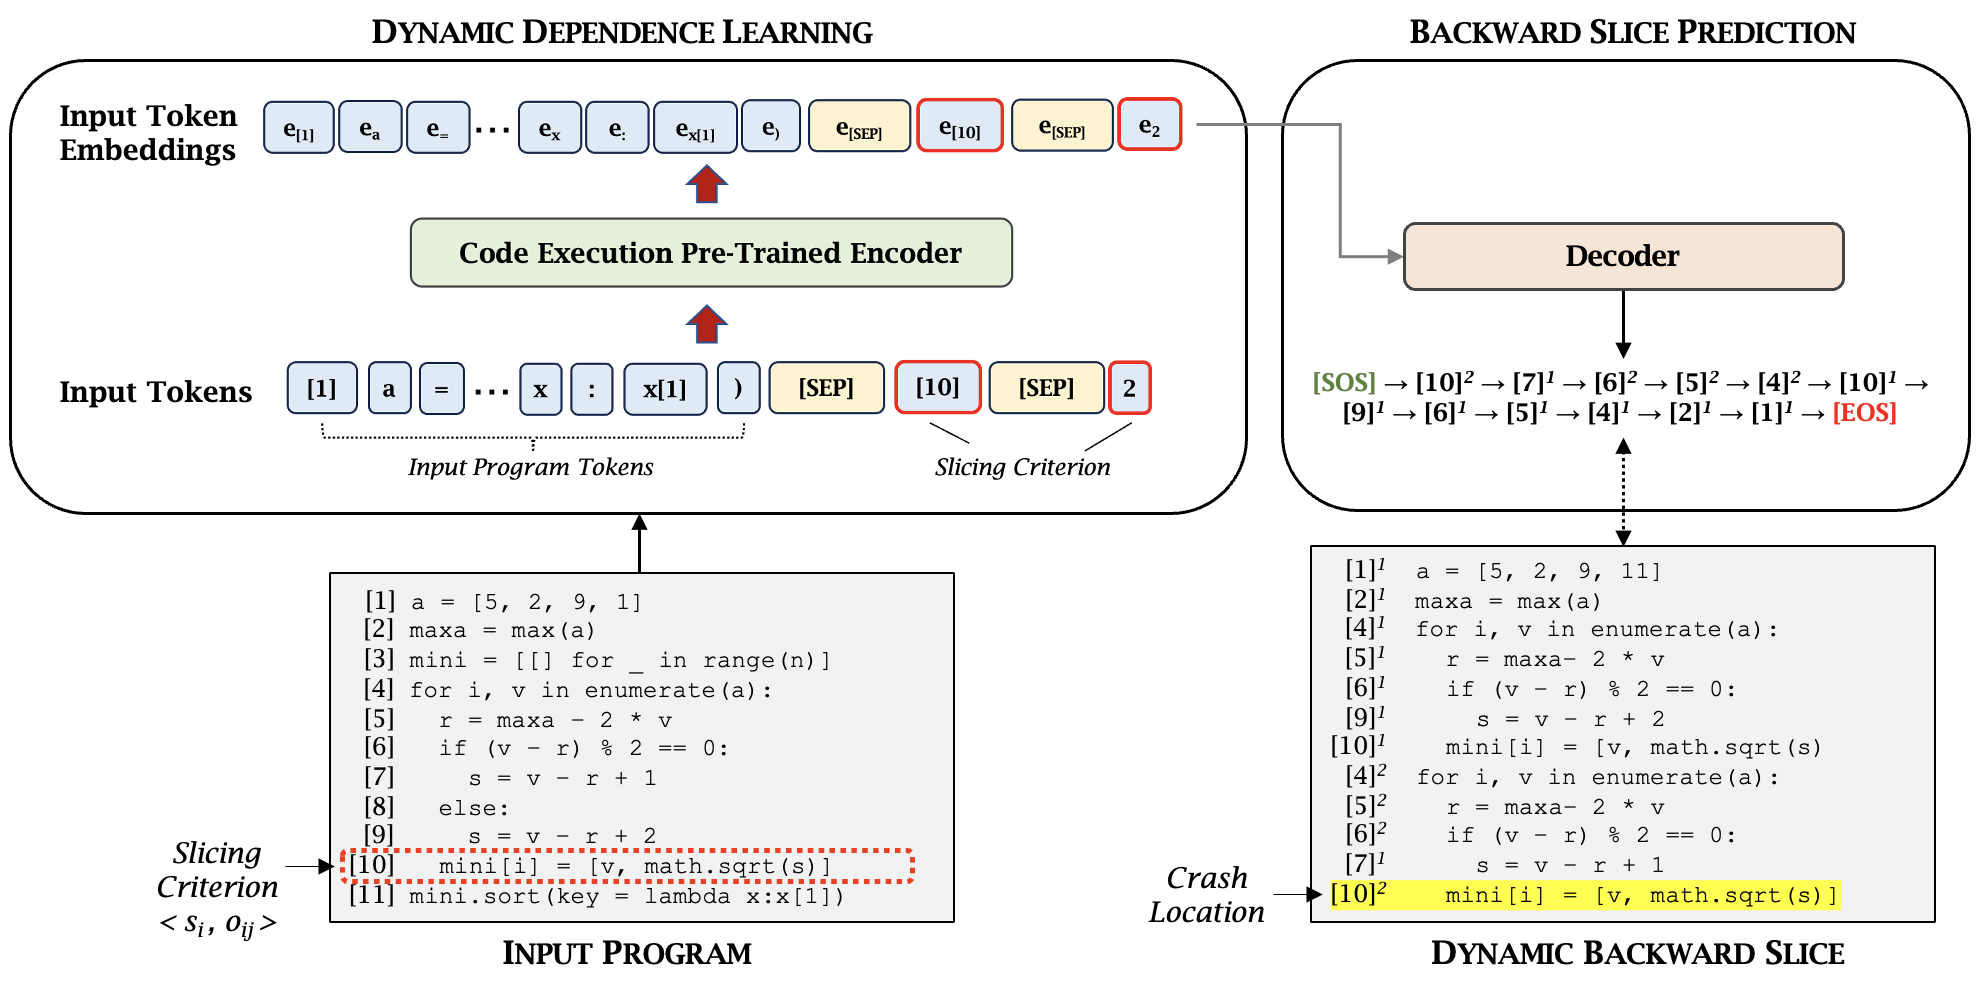
\includegraphics[width=5in]{dynamic-slicing.png}
\vspace{-12pt}
\caption{Predictive Dynamic Slicing}
\label{fig:dynamic-slicing}
\end{center}
\end{figure}

Given an (in)complete program, its inputs, and a specific statement with its occurrence in the execution trace as the slicing criterion, {\tool} predicts the dynamic backward slice for the criterion. In Fig.~\ref{fig:dynamic-slicing}, we illustrate the model architecture for {\tool}.
%Broadly, it adopts the sequence-to-sequence framework for predictive slicing, with the following essential components:
%\subsubsection{Dynamic Dependence Learning}
%In recent times, specialized source code models~\cite{icse23, graphcodebert-iclr21} have highlighted the effectiveness of learning-based approaches in understanding data and control dependencies. However, their learning objectives do not focus on run-time behavior of code, limiting their suitability for predictive slicing. To address this challenge, we chose to leverage CodeExecutor~\cite{liu2023code}, a model pre-trained on code execution, as the encoder in our framework. This code execution pre-training equips {\tool} with the capability to {\em learn dynamic program dependencies}. Furthermore, treating source code as a sequence of tokens empowers such pre-trained models (PTMs) to operate efficiently for both complete and partial code, thereby overcoming the limitations of dynamic execution, which is typically applicable only to complete code.
Let us consider a program $P = \langle s_1, s_2, \cdots, s_{N}\rangle$, where $s_i$ represents a statement in the program. Note that the inputs to the program, $I_P$, are included as assignment statements at the beginning of the program. We represent each statement $s_i$ as a sequence of code tokens \(\langle [i], t_1^{(i)}, t_2^{(i)}, \cdots, t_{M_i}^{(i)}\rangle\), where $[i]$ represents the special {\em line identifier} token included at the beginning of every line. For a given slicing criterion $\langle s_c, o \rangle$, that denotes the task of predicting the slice for the $o$-th occurrence of the statement $s_c$ in its execution history, the inputs to the encoder in {\tool} are as follows:

\begin{center}
$\{ [1], t_1^{(1)}, t_2^{(1)}, \cdots, t_{M_1}^{(1)}, \cdots, [\text{N}], t_1^{(N)}, t_2^{(N)}, \cdots, t_{M_N}^{(N)}, [\textbf{SEP}], [c], [\textbf{SEP}], o \}$
\end{center}

For each token $t$ in this input representation, the DDL module generates a contextually enriched token representation $e_t \in \mathbb{R}^d$ (where $d$ is the model dimension) with the following goals: (1) $e_t$ is syntax, semantics, and execution-aware; (2) it learns the execution-flow based on the model input tokens $t_x \in I_P$; (3) it learns the dynamic data and control dependencies between $t_j \in P$ and $t^{(c)}$ based on the occurrence of the slicing criterion denoted by $[c]$ and $o$, respectively.

\subsubsection{Backward Slice Prediction}
The primary challenge in predicting backward slices lies in ensuring that the sequence of statement/line occurrence aligns with the actual execution history, where the output sequence captures all dynamic data and control dependencies on the slicing criterion. Given the proven effectiveness of the {\em attention mechanism} in propagating information of the input sequence to the decoder within the sequence-to-sequence framework, we chose to adopt the Transformer decoder in {\tool}.

The encoder in the DDL module maps the model input to a sequence of continuous representations $\mathbf{x} = \{ e_{[1]}, e_{t_{1}^{(1)}}, \cdots, e_{[SEP]}, e_{[c]}, e_{[SEP]}, e_o \}$. Given $\mathbf{x}$, the decoder generates an output sequence $\mathbf{y} = \{y_1, y_2, \cdots, y_k\}$ of symbols one element at a time. Here, each $y_k$ corresponds to the special line identifier token $[i]$ in the input representation. This process is auto-regressive, where the previously generated symbols are consumed as the additional input for generating the next.

%\subsection{Fragment-Level Vulnerability Detection}
\label{sec:fragment}

%Verdi {\em et al.}~\cite{verdi-tse22} discovered 99 commonly used
%C/C++ code snippets in S/O answers, which they determined to~be
%vulnerable via manual inspection.

Verdi {\em et al.}~\cite{verdi-tse22} manually inspected and reported
99 commonly used C/C++ code snippets in S/O answers as vulnerable.
However, due to their incomplete nature, code snippets cannot
automatically be analyzed for vulnerabilities. In this experiment, we
design an "in-the-wild" evaluation by: (a) first, leveraging \tool to
predict PDGs for the code snippets; (b) next, making use of the
predicted PDGs and VulCNN~\cite{wu2022vulcnn} to detect the vulnerable
code snippets in those S/O answers.

%that we can correctly identify.

%Such a design will help developers detect early the vulnerabilities in the code fragments on online forums.

\subsubsection*{\bf Data Collection}
(1) We have collected an /C++ dataset comprising of $\sim$50K methods,
26.3\% of which are vulnerable. We split this dataset with a
80\%-10\%-10\% ratio to train VulCNN. (2) Of the 99 vulnerable code
fragments collected by Verdi {\em et al.}, we collect 66 for which, we
leverage \tool to predict PDGs and generate program
semantics-capturing images for VulCNN (VulCNN uses a third-party tool
that does not work with 33~snippets).

\subsubsection*{\bf Experiment Setup}
First, for all C/C++ methods in the VD dataset, we extract PDGs via
Joern program analysis tool~\cite{joern-2014}. We then train VulCNN,
achieving an F-score of 65.66\% in VD for the test set. Next, we
leverage \tool that was trained on a C/C++ dataset to predict PDGs for
the code snippets. Finally, we input the 66 program
semantics-capturing images corresponding to the predicted PDGs to
%the fragments to
the trained VulCNN model for vulnerability detection.

%discover the number of correctly detected vulnerable code~fragments.

\subsubsection*{\bf Preliminary Experimental Results}
We observed that VulCNN correctly identifies \underline{14} out of the
66 code snippets as vulnerable. This is very encouraging to see
{\tool}'s usefulness in VD for real-world code snippets. Despite being
trained on a VD dataset and C/C++ dataset collected without any
connection to the manually inspected vulnerable code snippets in
Stack Overflow, {\tool}+VulCNN detects 14 of them. The 52 mis-detected
ones could be due to the inaccuracy of VulCNN.
%\begin{tcolorbox}
PDGs predicted by \tool helps an automated VD tool detect \underline{14} real-world vulnerable code fragments.
%\end{tcolorbox}

%We observed that VulCNN correctly identifies \underline{14} out of the
%66 code snippets as vulnerable. This result is very encouraging to
%show {\tool}'s usefulness in detecting vulnerabilities in the
%real-world code snippets. Despite being trained on a VD dataset and
%C/C++ dataset collected without any connection to the
%manually~ins\-pected vulnerable code snippets in Stack Overflow,
%{\tool}+VulCNN detects 14 of them. The 52 mis-detected ones could be
%due to the inaccuracies of {\tool} and~VulCNN.



%\input{sections/ccf20-Thrust1}

%\input{sections/ccf22-Thrust-evaluation}

%\section{Plan-to-Do: \Tthree}
\label{thrust3:sec}


\subsection{T3 Task 1. Code Representation Learning for DL-based Bug Detection (BD) Models}

We plan to use our Design Framework to advance CRL techniques
for DL-based BD approaches.
%a DL-based BD approach~\cite{yioopsla19}.
%We illustrate to improve current state-of-the-art BD approaches using
%effective code representation learning (CRL). Existing
%approaches~\cite{Pradel-2018,Wang-2016,Bian-2018,ayewah-2007} still
%have limitations in detecting bugs occurring multiple methods and
%suffer high false positive rates.
We designed a BD {\bf specialized CRL} {\em capturing contexts in
  method bodies and relations among methods}~\cite{yioopsla19}.  Our
initial design has three main steps (Figure~\ref{Fig.2}): (1)
\textbf{Attention-Based Local Context Representation Learning}.  
Our model extracts long paths over the AST built from the method's body.
%A path starts from a leaf node and ends at another leaf node and
%passes the root node of the AST, as the leaf nodes in an AST are
%terminal nodes with concrete lexemes.
The nodes in a path are encoded into a continuous vector via Word2Vec
and the vectors are fed into two layers: attention-based GRU (att-GRU)
layer~\cite{Cho-2014} and attention Convolutional (att-Conv)
layer~\cite{Yin-2016}. The GRU layer allows our model to encode and
emphasize on the order of the nodes in a path. The att-Conv layer
allows our model to emphasize and put more weights on buggy paths.
Then, we use Multi-Head Attention~\cite{Vaswani-2017} to combine the
result from att-GRU layer and att-Conv layer together as the
\textbf{path local context} representation.
%
\begin{wrapfigure}{r}{0.6\textwidth}
	\vspace{-13pt}
	\centering
	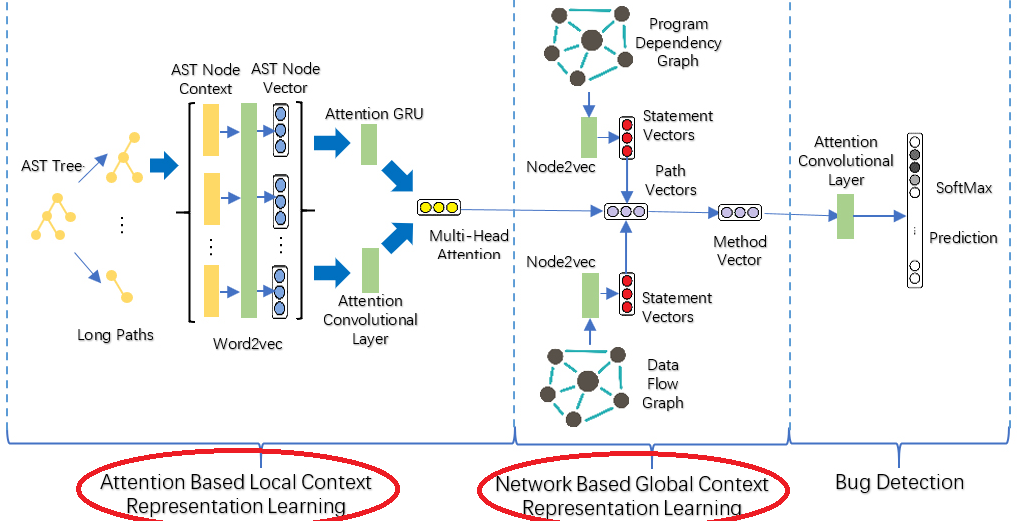
\includegraphics[height = 1.98in]{graphs/Graph_2_trim.png}
	\vspace{-22pt}
	\caption{Using Representation Learning for Bug Detection}
	\label{Fig.2}
%	\vspace{-10pt}
\end{wrapfigure}
(2) \textbf{Network-Based Global Context Representation Learning}.  We
also encode the method's context by building the PDG and the DFG
relevant to the method.
%We call them the \textbf{global context} as they provide the relations
%between the given method and other relevant methods in the project.
We use the Node2Vec~\cite{Grover-2016} to encode the PDG and DFG into
embedded vectors. These two vectors are combined by the space vectors
of all nodes in each path. We use matrix multiplication and convert
results together to get the path representation vector. Then, we can
have a method representation by appending all paths' vectors for each
method.  (3) \textbf{Bug Detection}. With both contexts for a method,
a classifier decides if the method is buggy or not. 

We plan to (1) investigate new CRL via our
framework to integrate program slices/reduction, symbolic traces, code
abstraction and intermediate representations; (2) explore new
embeddings and learning models for different level detection; (3) study new DL models on vectors from CRL to identify bugs.

%Our preliminary results~\cite{oopsla19} showed that with
%representation learning mechanisms (Figure~\ref{Fig.2}), our model
%significantly outperforms the one with the off-the-shelf
%Word2Vec-based CRL.

%\begin{wrapfigure}{r}{0.57\textwidth}
%	\vspace{-10pt}
%	\centering
%	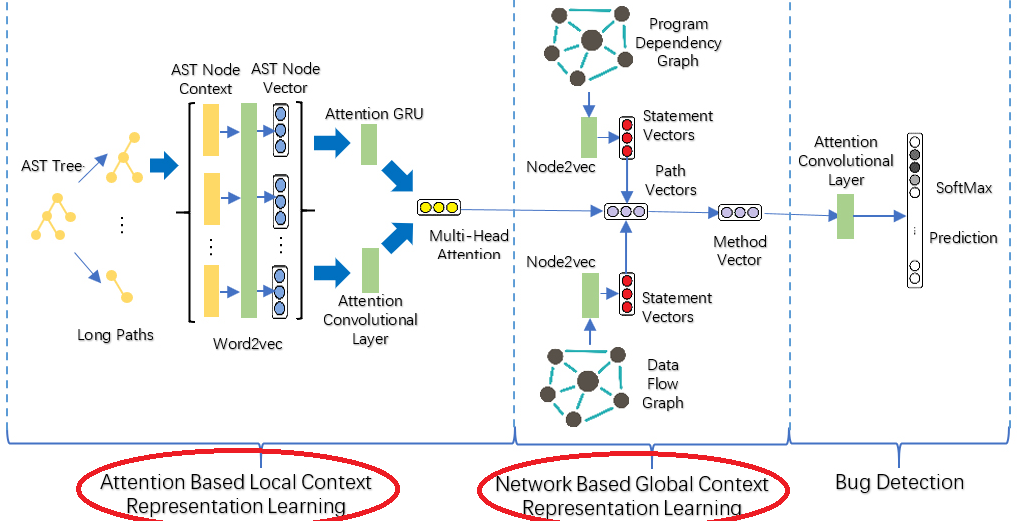
\includegraphics[scale=0.265]{graphs/Graph_2_trim.png}
%	\vspace{-25pt}
%	\caption{Using Representation Learning for Bug Detection}
%	\label{Fig.2}
%	\vspace{-15pt}
%\end{wrapfigure}

%Tien removed
%Table~\ref{allresults} show that (1) \textbf{our initial design
%  outperforms state-of-the-art baselines in detecting bugs},
%relatively improving DeepBugs, Bugram, NAR-miner, and FindBugs by
%69\%, 25\%, 92\%, and 156\% respectively in terms of F-score. (2)
%\textbf{our CRL with local and global contexts is more suitable than
%  existing CRL in bug detection}. It can improve relatively over all
%CLR baselines: DeepSim, DL-similarity, code2vec, Tree-based LSTM, Code
%Vectors,and GGM by 67\%, 38\%, 82\%, 206\%, 101\%, and 16.3\%,
%respectively, in terms of F-score. Importantly, our false positives
%rate is lower than others.
%\begin{wraptable}{r}{0.7\textwidth}
%	\vspace{-15pt}
%	{\footnotesize	
%		\caption{Ours Compared with BD Baselines and Existing CRL on BD. FP: False Positives}
%		\vspace{-10pt}
%		\begin{center}\label{allresults}
%			\renewcommand{\arraystretch}{1}
%			\begin{tabular}{p{1.2cm}<{\centering}|p{0.8cm}<{\centering}|p{0.8cm}<{\centering}|p{0.8cm}<{\centering}|p{1cm}<{\centering}|p{0.8cm}<{\centering}
%					|p{0.8cm}<{\centering}|p{0.8cm}<{\centering}|p{0.8cm}<{\centering}|p{0.8cm}<{\centering}|p{0.8cm}<{\centering}|p{0.8cm}<{\centering}} \cline{2-12}
%				
%				
%				\hline
%				\multirow{2}{*}{Category}& \multicolumn{5}{c|}{Bug detection baselines} & \multicolumn{6}{c}{Existing CRL on bug detection}\\
%				\cline{2-12}
%				& \textbf{Ours} & \textbf{DB} & \textbf{Bram} & \textbf{NARM} & \textbf{FB}   &\textbf{DS} & \textbf{DLS} & \textbf{C2V} & \textbf{TL} & \textbf{CV}&\textbf{GGM}\\
%				\hline
%				Recall  & 0.68 & 0.62 & 0.64 & 0.72 & 0.76   & 0.67 & 0.71 & 0.69 & \textbf{0.82} & 0.70&0.73\\
%				Precision& \textbf{0.39} & 0.25 & 0.32 & 0.11 & 0.08  &  0.19 & 0.24 & 0.17 & 0.09 & 0.15&0.30\\
%				F-score & \textbf{0.50} & 0.36 & 0.43 & 0.19 & 0.14 & 0.30 & 0.36 & 0.27 & 0.16 & 0.25&0.43\\
%				FP Rate & \textbf{0.21} & 0.41 & 0.39 & 0.52 & 0.66 & 0.35 & 0.36 & 0.43 & 0.69 & 0.45&0.28\\
%				\hline
%			\end{tabular}
%			DB=\deepbugs~2018: A deep learning bug detector; Bram=\bugram~2016: A n-gram model based detector;
%			NARM=\narminer~2018: A rule-based static detector mines negative rules on the code;
%			FB=\findbugs~2007: A rule-based static detector encoding +300 bug patterns.
%			DS, DLS, C2V, TL, CV, and GGM are defined in \textbf{Table 2}.
%			
%		\end{center}
%		\vspace{-25pt}
%	}
%\end{wraptable}

%Our initial results confirm that effective code representation learning (CRL) can help improve bug detection.



%Besides the basic CRs, e.g., identifiers/tokens/data and control
%flows/program dependency graph, we plan to investigate code
%representations obtained from more program analysis techniques (static
%and dynamic), such as program slices/reduction, symbolic traces, code
%abstraction, code intermediate representations (IR). Then, we combine
%the basic ones with the representations obtained from more static and
%dynamic program analysis techniques.  (2) Exploring new embeddings and
%learning models to propose new CRL approaches specialized for bug
%detection at different levels (i.e., variables, statements, and
%methods).  (3) Studying and proposing new deep neural networks on code
%vectors generated from CRL to identify bugs.


\subsection{T3 Task 2. Test Code Representation Learning for Regression Testing in CI}

%We use code representation learning to improve the
%selection and prioritization of test cases in Continuous
%Integration (CI)~\cite{duvall2007continuous}.
%
Regression Testing (RT) in Continuous
Integration~\cite{duvall2007continuous} (RT-CI) differs from the
traditional RT because most traditional RT techniques cannot be
applied at the scale of modern CI
practices~\cite{elbaum2014techniques} that require frequent commits to
the shared code base and cause the cost of continuous RT escalate
dramatically~\cite{memon2017taming}.
%
%RT-CI requires to identify and prioritize a subset of test cases that
%can timely and effectively uncover potential regression faults in the
%latest committed changes.
%
%Test selection and prioritization approaches in RT-CI are
%mainly in two directions: heuristics-based approaches
%(e.g.,~\cite{elbaum2014techniques,gligoric2015practical,yu2018study})
%and machine learning based approaches. However, existing approaches,
%e.g.,~\cite{bertolino2020learning,spieker2017reinforcement} still have
%limitations in accuracy and scalability as they lack the learning of
%deep features of test cases and source code and their relations.


%^Both only selection without prioritization or vise versa may be
%unsatisfactory, as time intervals among commits are very short and not
%all selected tests can be run or avoiding running many non-failing or
%irrelevant tests is the goal.
We will design a deep learning approach that leverages code representation
learning to select test cases and then prioritizes them in
each CI cycle.  
(1) \textbf{Test Selection.}  We use a hybrid strategy to select a subset of test cases, considering
static class-level dependencies among test cases and the ones between
changed source code and test cases, newly added test cases, diverse
test cases (e.g., \cite{jiang2009adaptive,henard2016comparing}). 
Static techniques are preferred over dynamic ones that are impractical
in CI due to runtime overhead~\cite{bertolino2020learning}. 
(2) \textbf{Test Prioritization.} Unlike previous approaches
(e.g.,\cite{bertolino2020learning}) modeling source code and test
history using hand-crafted metrics, we use CRL techniques (e.g.,
preferably unsupervised word embedding algorithms such as
Word2Vec~\cite{word2vec}, ELMo~\cite{peters2019knowledge},
FastText~\cite{bojanowski2017enriching}) to learn deep features of the
code under test to vectors, selected test cases, annotations for tests in code, 
similarities between
test cases and changed code, history-based test information (e.g., the
failed tests in the current commit and their similarities with the
changed code, the failed tests per test class in previous commits
before the current one, execution times).  Then, we utilize
learning-to-rank framework or active learning to prioritize test cases. 
In terms of
time complexity, existing approaches still have to generate graphs
(e.g., call/control graphs) for building metrics in a cycle, which can
take a longer time. In our approach, we build a language model
off-line and apply it on the natural sequences (or just tokens or AST)
of code under test into a vector in a cycle, which may not add overhead and even faster.  
Based on our previous experience, CRL can generate deeper and more representative
features than the hand-crafted metrics, leading to better results. 
We will further (1) investigate different
strategies for selection with CRL; (2) explore new fast and efficient
embeddings and learning models to propose new CRL approaches
specialized for RT-CI; (3) study to propose new practical
CRL-based approaches for test prioritization.



%study to propose a new off-line training for costly but potentially useful features and on-line prediction approach. 


%We exclude coverage-test selection and prioritization as they are very costly in CI due to the costs of instrumentation, recording and maintaining coverage data per release, in addition, they provide low accuracy due to the quick cycles and code changes


%different relationships: test cases dependency, dependency between test cases and source code, source code analysis for selecting and prioritizing test cases


\subsection{T3 Task 3. Code Coverage RL, Relation RL, and CRL for Fault Localization}

\begin{wrapfigure}{r}{0.45\textwidth}
	\vspace{-12pt}
	\centering
	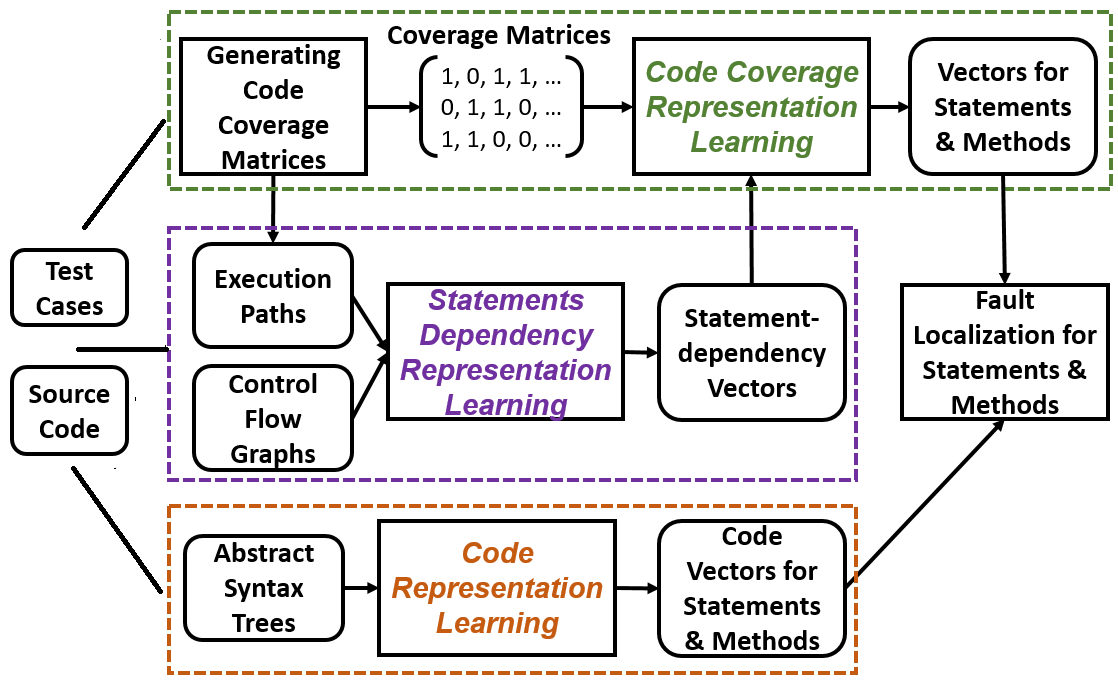
\includegraphics[height=1.8in]{graphs/newOverview}
	\vspace{-20pt}
	\caption{Using Representation Learning in FL.}
	\label{floverview}
	\vspace{-10pt}
\end{wrapfigure}
To experiment with CRL for dynamic information from program
executions, we propose a customized CRL for a fault localization
approach~\cite{icse_fl_21} at the statement and method levels.
%
%We use effective code and test coverage representation learning and
%novel deep neural networks for localizing faults at statement and
%method levels.
Our preliminary design~\cite{icse_fl_21} (Figure~\ref{floverview}) was
to leverage representation learning (RL) in three aspects. (1) {\bf
  code coverage representation learning}: Existing approaches
(spectrum-based, mutation-based, and deep learning-based approaches)
have never used the full details of test coverage, instead, they use
the spectrum and(or) mutation based formulas to summarize test
coverage for all test cases on each statement. We propose to {\em
  treat the FL problem as image processing by learning code coverage
  representations on the full details of the test coverage matrix}.
%Existing approaches (spectrum-based, mutation-based, and deep
%learning-based approaches) have never used the full details of test
%coverage, instead, they use the spectrum and(or) mutation based
%formulas to summarize test coverage for all test cases on each
%statement.
%To enrich test coverage matrices, we extract failing information of a
%test case and link it with specific code statements.  We use -1 for a
%failing test case at a statement exhibiting a crash or incorrect
%value.
%
%Next, while the rows representing statements are arranged according to
%the appearance order in the code, we order the columns, representing
%the test cases, so that the test coverages (i.e., the -1s, 0s, and 1s
%in the test coverage matrix) around the buggy statement would form a
%characteristic ``visual'' feature for a DL model to learn and detect
%it.  We directly perform RL on the improved matrices to learn vectors
%for statements or methods.  \underline{Second}, we integrate the
%dependencies/relations among the statements in the fault localization
%process using data dependency and execution traces.
(2) {\bf Statement dependency representation learning}: we aim to
learn the data/control dependencies among the statements. (3) {\bf
  code representation learning}: we also conduct CRL on sub-trees and
long paths of ASTs to generate vectors for source code. Finally, we
combine all three types of representation learning to represent a
statement or method by a vector representation. We will explore
different DL models for the classification purpose.~Preliminary
work shows that CNN works well for this classification of
a method/statement into buggy or not.

%(1) We prioritize test cases and mine failing information of test
%cases to enrich test coverage matrices and learn the code coverage
%representations; (2) We conduct the CRL on sub-trees and long paths of
%ASTs to generate vectors for source code, and also generate data flow
%graphs and run test cases to collect execution paths of code
%statements to learn the statement dependencies; (3) We combine the
%data flow graph and execution paths with improved matrices (spectrum
%and mutation), then apply a \cnn~on new matrices to learn vectors for
%an improved matrix.  We use another CNN on code vectors, vectors for
%the improved spectrum--based matrices, and vectors for the improved
%mutation-based matrices to perform fault localization (FL) at
%method-level. Our design can also work on statement-level FL by
%replacing the CRL at statement-level.


%\begin{table}[h]
%	\vspace{-15pt}
%	
%	{\footnotesize	
%		\caption{Our Approach Compared with FL Baselines at method-level and statement-level on Defects4J having 395 Bugs in total}
%		\begin{center}
%			\renewcommand{\arraystretch}{1}
%			\begin{tabular}{p{1cm}<{\centering}|p{0.8cm}<{\centering}|p{1cm}<{\centering}p{1cm}<{\centering}p{1cm}<{\centering}p{1.5cm}<{\centering}
%					p{1.2cm}<{\centering}p{1.5cm}<{\centering}|p{1.6cm}<{\centering}p{1.5cm}<{\centering}p{0.8cm}<{\centering}p{1.2cm}<{\centering}|p{0.8cm}<{\centering}} \cline{2-13}				\hline
%				\multirow{2}{*}{}& \multicolumn{7}{c|}{Fault Localization at Statement-Level} & \multicolumn{5}{c}{Fault Localization Method-Level}\\
%				\cline{2-13}
%				& \textbf{Ours} & \textbf{Ochiai} & \textbf{Dstar} & \textbf{MUSE} & \textbf{Metallaxis} &\textbf{RBF-NN} & \textbf{DeepFL-S} &\textbf{MULTRIC} & \textbf{FLUCCS} & \textbf{TraPT} & \textbf{DeepFL}&\textbf{Ours}\\
%				\hline
%				Top-1  & \textbf{74} & 17 & 19 & 26 & 24   & 16 & 36 & 80 & 160  & 156 & 213 &    \textbf{242} \\
%				MFR & \textbf{19.97}& 46.51 & 39.47 & 32.51 & 31.42 & 20.96 & 21.89  & 37.71 & 16.53 & 9.94 & 6.63 & \textbf{6.21}\\
%				\hline
%			\end{tabular}
%			RBF-NN: RBF Neural Network,
%			DeepFL-S: DeepFL with only features from spectrum+Mutation+MLP applicable to statements,
%			Top-1: the number of faults with a least one faulty element (statement or method) within top-1 position,
%			MFR: Mean First Rank of the localization of the first faulty element.
%			All method-level FL are machine learning (incl. deep learning) based.
%			\label{FL_S_M}
%		\end{center}
%		\vspace{-20pt}
%	}
%\end{table}


%Table~\ref{FL_S_M} show that our initial approach outperformed all baselines at both statement and method levels. Compared with the best performing statement-level and method-level baseline: DeepFL-S and DeepFL, we improved them by 115\% and 14\%, respectively. Our key ideas of designing representation learning for code and test coverage can help improve the current state-of-the-art FL research.

%To expand our initial design, we will (1) derive new code representations for FL; (2) Explore new embeddings and learning models to propose new code representation learning (CRL) approaches for FL; (3) Study and proposing new deep neural networks to localize faults.

\subsection{T3 Task 4. Code Transformation Learning for Automated Program Repair}

In this task, we aim to improve DL-based APR approaches via effective
CRLs, particularly {\bf Code Transformation Learning}.
%to improve the current deep-learning (DL) and pattern APR approaches
%using effective CRL and novel deep neural networks.  The DL-based
%approaches, e.g.,~\cite{hata2018learning,lutellier2020coconut}, still
%have limitations in learning bug-fixing code changes and learning
%which context of the surrounding source code that certain bug-fixing
%changes should be made.  These limitations lead to incorrect fixing
%locations or incorrect fixes.
We initially designed a two-tier DL model, \tool~\cite{icse_fl_20}, to
treat APR as code transformation learning from the prior bug fixes and
the surrounding code contexts of the fixes.
%
%For training, {\tool} has 5 key steps: {\bf (1) Pre-Processing.}
%First, {\tool} performs alpha-renaming on the names of variables
%within a method of a project.  Second, , {\tool} uses
%Word2Vec~\cite{Mikolov-2013} to train a vector representation for each
%unique token in a given pair of buggy method ($M_b$) and its fixed
%version ($M_f$).  {\tool} identifies the buggy sub-tree ($T^{sub}_b$)
%within $M_b$, and $T^{sub}_b$'s corresponding changed sub-tree
%($T^{sub}_f$) within $M_f$.  Finally, we used a code summarization
%model~\cite{wan-ase18} to summarize a tree into a vector for a node
%({\em a summarized node}). We obtain one vector for $T^{sub}_f$ and
%another one for $T^{sub}_b$.
{\bf (1) Code Context Learning.} We designed a two-layer learning model
that leans the code transformations for bug fixes and the context of
the code surrounding the fixes. The first one is dedicated for local
\textbf{C}ontext \textbf{L}earning \textbf{L}ayer (CLL).
%
For training at this layer, we replace the changed sub-tree with
a {\em summarized node}, as well as the buggy
sub-tree.  Given pre-processed pairs of methods, we developed a
tree-based encoder-decoder model using tree-based
LSTMs~\cite{tai2015improved} for this local context learning.  We
compute the vector for a method AST with the summarized node in a pair
of methods ($M_b$, $M_f$). The obtained vectors are used as the weights
in the next step. {\bf (2) Code Transformation
	Learning.}  The second layer is dedicated to code
\textbf{T}ransformation \textbf{L}earning \textbf{L}ayer (TLL) for
bug-fixing changes. In TTL, the changed sub-tree before and after the
fix is used for training to learn the bug-fixing code
transformations. Moreover, the context of the transformation computed
as the vector in the context learning layer is used as an additional
input in this~step.
%Specifically, we use the same tree-based encoder-decoder model in the
%first layer, CLL, to encode both structural and token changes.  {\bf
%  (4) Program Analysis Filtering.}  {\tool} derives the possible
%candidates using program analysis filters, including the filter to
%check the existence of variables, methods, and class names, the filter
%to convert the keywords back to the right names, and the filter to
%check the syntax of final result.  {\bf (5) Patch Re-ranking.} We use
%a CNN~\cite{kim2014convolutional} based classification approach to
%re-rank the generated possible patches based on the detailed
%contextual information, which helps better selecting the results.

We also have the following tasks in this thrust: (1) Investigating new
code representations for APR using our code representation learning
(CRL) framework; (2) Exploring new embeddings and learning
models to propose new CRL approaches specialized for APR; and (3)
Studying and even proposing new deep neural network models to auto-fix
multi-statements and multi-location bugs.

%In our initial design, our DLFix is novel in two ways: new CRL and a
%new two-layer tree-based encoder-decoder model.




%\input{benchmark}

%\input{model}
%\input{mudetect}

%\input{solution}


\section{Evaluation Plan}
\label{eval}

%Our {\em goals} of the evaluation plan include the studies to answer the questions:

%1) {\bf Intrinsic evaluation.} 

%2) {\bf Extrinsic evaluation.} How well do our proposed tools and methods help developers in improving the learning and usages of APIs in software libraries?

%3) How effectively do the proposed tools and methods help developers
%in real development processes?


\paragraph{\bf (1) Partial-Code Analysis Performance.} We aim
to evaluate how well {\tool} can provide the structural analysis and
semantic analysis for incomplete code fragments.  Assessing the
performance of \tool is not straightforward, mainly due to the lack of
ground-truth for partial code fragments. Thus, we could evaluate it on
programs in Java and C/C++ as follows.  First, we will train {\tool} on
complete code. For testing, we will treat each method individually and
choose a consecutive portion within the method to predict the actual
elements and dependencies, and compare them against the actual ones.
For example, in Thrust 1, if we evaluate the performance of structural
analysis infrastructure, we could compare the recovered/predicted code
structure in terms of ASTs against the actual ASTs of the original
code. For Thrust 2 in dependency analysis, we could treat each method
individually and choose a consecutive portion within the method to
predict the program dependencies, and compare them against the actual
dependencies. We will adopt the standard evaluation metrics, i.e.,
\textit{Accuracy}, \textit{Precision}, \textit{Recall}, and
\textit{F-Score}. $Accuracy = \frac{TN+TP}{TN+FP+TP+FN}$, $Recall =
\frac{TP}{TP+FN}$, $Precision = \frac{TP}{TP+FP}$, and $F{-}Score =
\frac{2*Recall*Precision}{Recall+Precision}$ where TP = True
Positives; FP = False Positives; FN = False Negatives; TN = True
Negatives.

\paragraph{\bf (2) Complete-Code Analysis Performance.}
We aim to compare the performance of {\tool} (AI/ML + PA) against the
traditional PA techniques in building structures and dependencies from
source code. We could collect a set of tools, e.g., to build the
program dependence graphs to obtain the benchmark. Then, we will
compare the results from {\tool} and other tools w.r.t. the
benchmark. We will also measure the time efficiency in building the
infrastructures such as ASTs or PDGs from all the tools under
comparison. We will use the same evaluation metrics as in the
experiments for incomplete code.

\paragraph{\bf (3) Usefulness Evaluation on Downstream Tasks.}

{\em We evaluate how well {\tool} helps in the downstream software
  engineering tasks for partial code}. For example, in bug and
vulnerability detection for code snippets, to evaluate the usefulness
of the PDGs predicted by \tool (say, PDG\textsuperscript{*}), we
will design experiments around the task of vulnerability detection at two
levels of granularity: complete code at the method-level, and partial
code at the snippet-level. For the method-level VD task, we leverage
any ML-based vulnerability detection tool, e.g.,
VulCNN~\cite{wu2022vulcnn}, an image-inspired DL-based VD model which
utilizes PDGs to predict whether a given method has vulnerabilities or
not. Here, we aim to estimate how well PDG\textsuperscript{*}s
predicted for the methods in the dataset approximate the performance
of the actual PDGs retrieved from a program-analysis tool. We could
use the same methodology for evaluating the usefulness of {\tool} in
other types of software engineering tasks.



%{\em in bug detection (BD), fault localization (FL), Regression
%  Testing in Continuous Integration (RT-CI) and automated program
%  repair (APR) approaches are in comparison with the state-of-the-art
%  approaches?}  First, we use the large-scale cross-language datasets
%with bug fixes.  To detect bugs, we will train our BD and FL
%approaches on buggy code with known buggy locations and non-buggy
%code. For APR, we train APR approaches on buggy code with its fixed
%versions to automatically learn fix patterns. Second, for evaluation,
%we follow prior research for BD, FL, and APR. \underline{In DB}, we
%will measure the precision, recall, F-measure, and the number of true
%bugs detected in Top-N (e.g., N=50). \underline{In FL}, we use the
%following: \textit{Recall at Top-N}, the number of faults with at
%least one faulty element located within the first N positions.
%\textit{Mean Average Rank (MAR)}: For precise localization of all
%faulty elements of each fault, we compute the average ranking of all
%the faulty elements for each fault.  \textit{Mean First Rank (MFR)}:
%For each project, we compute the mean of the first faulty element's
%rank for each fault.  \underline{In RT-CI}, we calculate APFD (Average
%Percentage of Faults Detected), Normalized APFD
%(NAPFD)~\cite{qu2007combinatorial} and Normalized Rank Percentile
%Average (NRPA)~\cite{bertolino2020learning}. Rank Percentile Average
%(RPA) was proposed to adapt the Average Fault Percentile to the
%prioritization problem for computing how much a predicted ranking is
%close to the actual ranking.  \underline{In APR}, we calculate the
%number of bugs automatically fixed and the ratio of correctly fixed
%bugs to the number of plausible patches when comparing with
%traditional APR approaches. Compared with DL ARP, we use: \textit{Top
%  K is the number of times that a correct patch is in the ranked list
%  of top K candidates, e.g., K=1,3,5}.

%\paragraph{{\bf (2) Comparative Study on Code Representation Learning (CLR) for BD, FL, RT-CI and APR.}}
%{\em Research question: How effective are our CRL for BD, FL, Testing and APR, and how well are they in comparison with the state-of-the-art approaches?} 
%We will perform controlled experiments to evaluate the effectiveness of our CRL in BD, FL, RT and APR, especially ablation studies on different factors in CRL. In addition, we will continue to compare our CRL with other existing CRL on other software engineering and program analysis topics. We use the same evaluation metrics as the ones in (1) for BD, FL, and APR.

%To evaluate our evaluation framework for CRL, we propose the following
%procedure. First, we will choose a well-known DL-based model for each
%application, BD, FL, RT-CI, and APR. For each of those DL-based
%models, we varied the CRL model using our design framework in Thrust
%1. We measure the quality of each CRL model and measure the
%performance of the DL-based model for each application. We will use
%statistical test to evaluate whether the high accuracy of CRL model
%leads to high performance of the same downstream model used in the
%application under study.

%\subsection{Evaluation on usefulness of the approaches in helping developers in learning API usages}

%We will perform controlled experiments to evaluate our methods and tools with developers in the loop using the actual system. We will
%gather developers and provide them various programming tasks, and
%compare the efficiency of their work with our methods/tools to the
%baseline approaches, e.g., with the Web-based code search or other
%code synthesis approaches.

%We will measure the efficiency of the work using different methods
%based on the following evaluation metrics. First, we measure
%efficiency. This could be measured by the time for developers to
%perform the tasks or the number tasks completed by developers in a
%period of time. Second, we measure coding effort: how much effort that
%developers must do to complete the API usages given the API code from
%the methods. Third, we will measure semantic correctness, either by
%the number of passing test cases or by human judgements. Finally, we
%will perform surveys on the quality of the synthesized API usage code
%to get the feedback for future improvement in the next step.

\paragraph{\bf (4) Evaluation on proposed tools and methods in helping developers in real-world development.}

We will perform a set of user studies on the usefulness of our
proposed tools in the wild by releasing our
tools in the actual real-world development. 
%We will analyze all the aspects as in the previous studies and the total uptake of the tools.  
We will record feedback to improve our tools.
%PI Wang will connect with the Industry through our \textit{The New Jersey Innovation Institute} (NJII)~\cite{njii}, an NJIT corporation focusing on helping pri%vate enterprise.
UT-Dallas has a strong tie with companies like AT\&T, Facebook, and
Bloomberg. PI Nguyen will work with his existing collaborators in
Microsoft, IBM, ABB research to perform user studies on the groups of
developers in certain tasks to evaluate the usefulness of our proposed
tools.

%\section{Education and Dissemination Plan - Curriculum Development Activities}
\section{Dissemination and Educational Plan}
\label{edu}

\paragraph{Engaging Students into Research}

This project will create opportunities for students at UT-Dallas to
participate into cutting-edge research: PI Nguyen has currently supported
four female students (2 PhD students and 2 undergraduates), with a total
of four PhD students, two M.Sc. students, and four undergraduates.

%has worked with 6 undergraduate students (i.e., two are female
%students) and two master students (i.e., independent
%study). Additionally, PI Wang is actively doing research with a group
%of two undergraduate students (Vrushali Koli (female) from NJIT and
%Delmond Wyllis from Rowan Univ. in NJ) and \underline{six high-school
%students} in the NJ Governor's STEM Scholars Program.  PI Wang
%supervise 4 Ph.D students (one female) and 1 master student.


%(2) {\em UTD's Collegium Honors Program}:
%{\em ISU's Freshman Honor program}: 
%PI Nguyen has been engaging two freshman honor students into his
%research program since he joined UTD in 2016. 
%REU supplements will be requested to support this undergraduate research; 
%
%(3) {\em HackersUTD}: This Fall, UT Dallas Computer Science department
%welcomed 2,876 students, including 466 CS/software engineering
%freshmen, with activities and events as a way to welcome and
%familiarize students with the UT Dallas CS. We will engage members of
%this organization; 
%(3) UT Dallas works with North Texas high school
%seniors to host IT empowerment for their camps. To generate interests
%in computing studies from {\em high-school} students in Dallas area,
%we will involve them in design projects that target the use of
%software in teaching {\em K-12} subjects; 
%(2) {\em UTD's Women Who
%Compute}: The PI Nguyen has actively used this program to generate interests
%in SE research from women students. From the past, PI Nguyen has
%mentored 3 women students; 
%(Dong Fei, Kristina Gervais, Taylor Schreck); 
%(3) {\em Involving Under-represented Minorities}: We
%will attract minority students funded by GEM fellowships, involve
%high-school teachers via Alliances for Graduate Education and the
%Professoriate.
%and UT Dallas Programs for Minors: we will work
%with this program to recruit more student in minority.

%This project will also create opportunities for students at UT-Dallas:
PI Nguyen has extensive experience in engaging students in
outreach programs: (1) {\em UTD's Collegium Honors Program}: He
has been engaging several freshman honor students into his research
program since 2005. (2) {\em HackersUTD}: In Fall'19, UT Dallas CS
welcomed 2,876 students, including 466 freshmen, with activities and
events as a way to familiarize students with CS/SE. We will use the
results of this project in this program.
%
(3) UT Dallas works with {\em North Texas high school seniors to host
IT empowerment} for their camps. To generate interests in computing
studies from {\em high-school} students in Dallas area, PI Nguyen has
been involving them in design projects that target the use of software
in teaching {\em K-12} subjects; (4) {\em UTD's Women Who Compute}: he
has actively used this program to generate interests in SE research
from women students. PI Nguyen has mentored several {\em female
undergraduate students} (Weining Gao, Kristina Gervais, Taylor
Schreck, etc.); (4) {\em Involving Under-represented Minorities}: We
will attract minority students funded by GEM fellowships, involve
high-school teachers via Alliances for Graduate Education and the
Professoriate; and (5) {\em UT Dallas Programs for Minors}: we will
work with this program to recruit more student in minority.


\paragraph{Dissemination of Research and Teaching Materials}

Beside publications at professional \emph{conferences, journals} and
public Web sites, we will use the available resources at UT-Dallas
through various forums for dissemination.
%
%PI Wang is a member of DIMACS~\cite{dimacs}, the Center for Discrete
%Mathematics and Theoretical Computer Science as an NSF-funded Science
%and Technology Center (STC) and a New Jersey Commission on Science and
%Technology Advanced Technology Center. DIMACS has over 350 members
%across the U.S. PI Wang will continue to advocate our research through
%DIMACS events, research and academic programs.  PI Wang will use
%the \textit{annual NJIT Research Showcase and President Forum} to show
%our accomplishments to all NJIT people.
PI Nguyen will continue to use the following resources: (1) TExAs
Software Engineering Research (TEASER) Doctoral Symposium: where SE
researchers from the DFW Metroplex (and beyond) meet to discuss and
work on SE topics.  The mission of TEASER is to provide a supportive
space in which PhD students can present and receive feedback on their
research work, while at the same time giving both researchers and
students a venue to get to know one another and network productively.
(2) American Society for Engineering Education: PI Nguyen, with his
prior NSF-funded TUES project, has disseminated educational results
via this channel.
%He will continue to disseminate educational outcomes via this
%educational society.
(3) Leadership through Engineering Academic Diversity (LEAD): PI
Nguyen have served as mentors for this program which aims to enrich
educational experience of {\em minority engineering students}.

\paragraph{Research Community Building.}

PI Nguyen has successfully organized the 1st {\bf International
Workshop on Representation Learning for Software Engineering and
Programming Languages (RL+SE\&PL 2020)}~\cite{rlsepl}, associated with
ESEC/FSE'20. The workshop had 104 paid registers and featured one
keynote speaker (Dr. Miltos Allamanis, well-known CRL scientist at
Microsoft Research) and six technical presentations. RL+SE\&PL'20 has
sparked constructive and inspiring discussions. With its success, we
are building a diverse and active community. We plan to build on the
success of the first edition to continue this series to disseminate
ideas to a wider community, and to build a larger community bridging
SE and ML.


\noindent {\bf Undergraduate and Graduate Software Engineering (SE) Education.} 
%PI Wang teaches fundamental and core SE courses NJIT: Building Web Applications (IS218) and System Design (IS390).
PI Nguyen is one of the key SE faculty members in SE at UT Dallas. 
%
He is one of the faculty who has initiated the
Undergraduate SE Program when he was at Iowa State University.
%He has
%successfully introduced several courses including Software
%Architecture and Design (CprE339) and Software Project Management
%(CprE329). 
Taking advantage of this project, PI Nguyen will introduce a deep
learning component and a new course in NLP+SE.
%The key teaching philosophy in this course is the combination of theory and practice.
%in which students will be introduced different principles and theories in the application of NLP in SE artifacts. 
%The tentative modules include 1) basic principles, processes, and paradigms in NLP, 2) programming languages versus natural languages, 3) API usages and reuse, 4) Statisical models used in SE applications, 5) machine translation and code migration, 6) language models for source code, 7) applications of machine translation in SE, 8) word embeddings and SE applications, 9) deep learning and SE applications, etc.
%\noindent {\em Graduate SE Education} 
PI Nguyen will teach a newly developed course, 
Selected Topics on AI in SE and PL,
including relevant topics to this proposal, e.g, 
AI in bug detection, fault localization, automated repair. 
%The PI Nguyen works
%with other UTD faculty to develop a series of six to seven SE graduate
%courses that will be offered at least every semester. This year, the
PI Nguyen introduced a new graduate level course on ``AI/ML for
Code''. The PI will introduce a new graduate course on the topic of
NLP+SE.
%Tools developed by this research will be used in class projects. 
The course will focus on SE advanced methods that
aim to help advance SE with AI/ML. 
The tentative topics include 1) program analysis, 2) code
analysis with AI/ML, 3) cross-language analysis between texts and code,
4) AI/ML for code, etc.
%4) code and text retrieval in SE applications, 
%3) NLP techniques and
%type inference, 4) NLP and de-ofuscation, 5) bug-fixing and
%machine learning.




\section{PI's Prior Relevant NSF Supports and Qualifications for this Project}
\label{prior}

%PI Wang has no prior relevant NSF supports.
%His relevant work on improving software maintenance, quality and reliability has been published in
%OOPSLA~\cite{yioopsla19}, ASE~\cite{son-2019-ase}, EMSE~\cite{noei2019towards,wang2016improving}, ICWS~\cite{venkatesh2016client}, ICSOC~\cite{wang2014developers}, and MSR~\cite{wang2013improving,wang2019extracting}.
%two ICSE submissions, and one PLDI submission.
PI Nguyen. CCF-1723215, \$260,709, 07/01/16-30/06/21, ``Collaborative
Research: Exploiting the Naturalness of Software''.
%
\noindent {\bf Intellectual Merit.} The work has the following
thrusts: (1) investigating NLP techniques for SE
applications, and (2) Developing a statistical machine translation
model for language migration.
%Investigating the integration of semantic information
%including data types, semantic roles, etc., into a language model, (2)
%Developing an accurate code-completion tool using statistical semantic
%language model, and (3) Developing a statistical machine translation
%model for language migration.
%
\noindent {\bf Broader Impact.}
%We developed practical software engineering tools, using statistical
%NL techniques for (a) code suggestion, completion, and correction
%tools, (b) assisting tools for programmers, (c) summarization, (d)
%retrieval, and (e) porting tools.
%The project has several publications at top-tier SE
%conferences, e.g., ICSE, FSE, ASE, TSE.
%including ICSE
%papers~\cite{icse05,icse07,icse09,icse10,icse11}, FSE
%papers~\cite{fse06,fse09,fse11}, ASE
%papers~\cite{ase06,ase08,ase08-2,ase09,ase10,ase11-phpsync,ase11-bugscout,ase11-idiff},
%OOPSLA papers~\cite{oopsla04,oopsla06,oopsla10}, and TSE
%papers~\cite{tse08,tse11}.
%
He has been awarded {\bf 4 ACM SIGSOFT Distinguished Paper Awards, one
  Best Paper Award, and one best ICSE Formal Research Demonstration
  Award} at the top-tier SE conferences including ICSE, FSE, and ASE,
one {\bf IEEE TCSE Distinguished Paper Award}. He has served on
Program Committees and Program Boards of ICSE, FSE, ASE, OOPSLA,
ECOOP. PI Nguyen was a Program Co-Chair of ASE'17. Since 2005, PI
Nguyen published at the top-tier Software Engineering conferences: 25
ICSE full papers, 15 ESEC/FSE full papers, 14 ASE full papers, 3
OOPSLA full papers.
%From Google Scholar, PI Nguyen's H-index
%is 49, Citations: 9,431, Citations in past 5-years: 5,879.
From CSRankings, he is ranked at the 3rd place among all US SE researchers in the past 10 years.

%making software development more accessible, enjoyable and productive;
%and therefore will broadly enhance the value that software
%professionals deliver to business and society.

%Dr. Nguyen is currently the PI of the NSF-funded project, ``
%Collaborative Research: Exploiting the Naturalness of Software'', that
%will end August 2018. The work has three thrusts of research.  (1)
%Investigating the integration of semantic information including data
%types, semantic roles, etc., into a language model, (2) Developing an
%accurate code-completion tool using statistical semantic language
%model, and (3) Developing a statistical machine translation model for
%language migration. So far, the majority of the tasks have been
%%completed except empirical evaluation in a real-word setting is
%needed.



%Several papers on our results were published through ICSE
%2010~\cite{icse10}, ASE 2010~\cite{ase10}, OOPSLA
%2010~\cite{oopsla10}, ICSM 2010~\cite{icsm10}, ICSE
%2011~\cite{icse11,nier11-1,nier11-2}, FSE 2011~\cite{fse11}, ASE
%2011~\cite{ase11-phpsync,ase11-bugscout,ase11-idiff}, and an IEEE TSE
%journal article~\cite{tse11}.

%Our next phase will be involved more with the tasks (2) and (3).

%Dr. Nguyen is currently an PI on a NSF-funded project: \#CCF-1018600,
%``Find and Fix Similar Software Bugs'', 08/15/2010 through
%07/31/2013. In this project, an empirical study will be conducted to
%collect, analyze, and understand the nature and characteristics of
%recurring and similar bugs within one and across multiple
%systems. This project is expected to advance software engineering
%knowledge on the theoretical foundation, concepts, practical
%techniques, and automated tools to (1) capture the characteristics and
%measure the similarity of code units involved in prior known fixed
%bugs, (2) identify the locations of potential buggy units and derive
%the guidelines to fix them by matching them to the relevant peer code
%units of the known bugs, and (3) support the similar bug detection and
%fixing process. Teaching modules and validation efforts in this
%project will involve students and professionals, promoting teaching
%and training software quality assurance.

%Dr. Nguyen is an expert in software building, software configuration
%management (SCM), and software refactoring. His research work on SCM
%has been published at various prestigious software engineering
%journals and conferences including clone-aware configuration
%management and operation-based version control (TSE'11~\cite{tse11},
%FASE'10~\cite{fase10}, ASE'09~\cite{ase09}), software
%refactoring-aware SCM and software merging (TSE'08 \cite{tse08},
%ICSE'07~\cite{icse07}, FSE'06~\cite{fse06}, OOPSLA'06
%demo~\cite{oopsla06}), object-oriented configuration management
%(ICSE'07~\cite{icse07}, WWW'06~\cite{www06}, ICSE'05~\cite{icse05},
%ICSM'05~\cite{icsm05}).

%His other software maintenance works include clone-related bug
%detection (TSE'11 \cite{tse11}), bug localization
%(ASE'11~\cite{ase11-phpsync}), bug localization from bug reports
%(ASE'11~\cite{ase11-bugscout}), recurring bug detection
%(ICSE'10~\cite{icse10}), API misuse detection
%(OOPSLA'10~\cite{oopsla10}, FSE'09~\cite{fse09}), recurring
%vulnerabilities detection (ASE'10~\cite{ase10}), etc.




%Since 2005, his work has been resulting several publications at
%top-tier SE conferences including 5 ICSE
%papers~\cite{icse05,icse07,icse09,icse10,icse11}, 3 FSE
%papers~\cite{fse06,fse09,fse11}, 8 ASE
%papers~\cite{ase06,ase08,ase08-2,ase09,ase10,ase11-phpsync,ase11-bugscout,ase11-idiff},
%2 WWW papers~\cite{www04,www06}, 3 OOPSLA
%papers~\cite{oopsla04,oopsla06,oopsla10}, and 2 FASE
%papers~\cite{fase09,fase10}, 2 TSE papers~\cite{tse08,tse11}.


\newpage
\setcounter{page}{1}
\pagenumbering{roman}

\bibliographystyle{IEEEtran}
%\nobibliography{oopsla19,icse20,FL,ref,autofixTools}
\bibliography{references,oopsla19,icse20,FL,ref,autofixTools,testPri,embeddingEva,reference,icse21IntVD,icse18,references-fuzzwise-1,references-fuzzwise-2}

%\bibliography{oopsla19, icseAutoFix20,bibliography,icse18,t2api17,ccf18,refs,securesync,tc10,tien,ccf09,ase10,ccf12,anomalies,completion,groums,usagemining,pattern,urls,other}

\end{document}
